%!TEX program = xelatex
\documentclass[WordOneHalf]{XDUthesis}
% 参数设置:
%     功能设置:
%         <nologo>:      封面页去除logo(默认有logo)
%         <WordOneHalf>: Word 1.5 倍行距(近似)(默认关闭)
%         <contentsnd>:  目录去除点的连接
%         <print>:       启用打印样式
%     以下为字体设置,仅在XeLaTeX和LuaLaTeX下有效;不设置由系统自动检测【Windows:windowsn, mac:mac】
%         <windowsn>: 由工作手册指定的字体设置,xelatex 下复制会乱码(不影响打印)
%         <windowsf>: 宋体的粗体版本由华文中宋替代,PDF复制不会有乱码;粗体黑体会有乱码
%         <adobe>:    采用对应的Adobe宋体和黑体作为中易宋体和黑体的替代;PDF复制无乱码
%         <mac>:      Mac系统下的字体
% 

\title{有限自动机C++工具箱等价性和最小化类软件测试}
\author{胡双朴}
\date{2019年06月01日}
%题目拆分:用于封面
\septitleA{有限自动机C++工具箱}%如果论文题目长度<=11中文字符只需填此项即可B项空着
\septitleB{等价性和最小化类软件测试}%如果论文题目长度>11中文字符, 建议拆分为10+x or 11+x 将剩余x个字符填在此处。
\class{\phantom{22}1504012\quad}%班级号
\schoolnumber{15040120169}%学号
\major{机械设计制造及其自动化}%专业
\school{机电工程学院}%学院
\supervisor{段江涛}%指导老师

% \usepackage[BoldFont]{xeCJK}
% \usepackage{courier}

\graphicspath{{./Figure/}} %%% 设置图片目录
\definecolor{codegreen}{rgb}{0,0.6,0}
\definecolor{codegray}{rgb}{0.5,0.5,0.5}
\definecolor{codepurple}{rgb}{0.58,0,0.82}
\definecolor{backcolour}{rgb}{0.99,0.99,1.0}

\lstdefinestyle{mystyle}{
    backgroundcolor=\color{white},   
    %commentstyle=\color{black},
    commentstyle=\color{XDU@commentcolor},
    keywordstyle=\color{magenta},
    numberstyle=\tiny\color{codegray},
    stringstyle=\color{codepurple},
    %basicstyle=\footnotesize\sffamily,
    basicstyle=\linespread{1}\small\ttfamily,
    breakatwhitespace=false,         
    breaklines=true,                 
    captionpos=b,                    
    keepspaces=true,                 
    numbers=left,                    
    numbersep=5pt,                  
    showspaces=false,                
    showstringspaces=false,
    showtabs=false,                  
    tabsize=4
}

\lstdefinestyle{mystyle2}
{
    showstringspaces=false,
    showspaces=false,
    tabsize=4,
    frame=lines,
    basicstyle = \footnotesize\XDU@codebasicfont,
    keywordstyle = \color{XDU@keywordcolor}\bfseries,
    stringstyle = \color{XDU@stringcolor}\ttfamily,
    commentstyle = \color{XDU@commentcolor}\rmfamily\itshape,
    breakatwhitespace=false,
    captionpos=b, 
    breaklines=true, 
    identifierstyle=,
    columns = flexible,
    numbers = left,
    numberstyle = \footnotesize\ttfamily
}

%%% 自动换行设置
\tolerance=1
\emergencystretch=\maxdimen
\hyphenpenalty=10000
\hbadness=10000

\usepackage{enumerate}
\usepackage{stmaryrd}  %toollbar
% \usepackage{bicaption}
% \usepackage{clrscode3e}

% \usepackage{algorithm}
% \usepackage{algpseudocode}

% \usepackage{program}

\begin{document}

% 摘要
%!TEX root = ../Demo.tex
% 中文摘要
\begin{abstract}
  本文对有限自动机 C++ 工具箱中的五个最小化算法进行功能测试。有限自动机 C++ 工具箱对 Hopcroft 算法(由 Hopcroft 提出)的实现需要输入数据为完全的确定性有限自动机。而对于其他三个最小化算法 HopcroftUllman 算法(由 Hopcroft 和 Ullman 提出)、 dragon 算法(由 Aho Sethi 和 Ullman 提出),Waston 算法(由 Bruce William Watson 提出)则没有明确要求数据数据是否是为完全的确定性有限自动机。除了 Brzozowski 的算法外,以上四个最小化算法都依赖于计算状态的等价关系(或可区分的关系),有限自动机 C++ 工具箱对 Brzozowski 算法的实现有一定的缺陷,在某些情况下会输出错误的结果。

  本文还为有限自动机 C++ 工具箱增加了用来计算从开始状态可以到达的状态的集合的算法(SReachable)、移除有限自动机中从开始状态不可到达的状态的算法(usefuls)和构造完全自动机的算法(complete)。

\end{abstract}
\keywords{确定性有限自动机, 最小化, 算法, 状态等价}

% 英文摘要
\begin{enabstract}
  This paper is just a sample example for the users in learning the \XDUthesis. I will try my best to use the commands and environments which are involved by the \XDUthesis. Also, the popular composition skills in figures, tables and equations will be elaborated.
  
  In the part unimportant, I will show something others, such as poems and lyrics.

\end{enabstract}
\enkeywords{XDUthesis, commands, environments, skills}

% 往PDF属性里面写下关键词信息
\makeatletter
\XDU@setpdf@keywords
%\make@abstract%
%
%\frontmatter
%\tableofcontents%
%\mainmatter
\makeatother

\maketitle

% 文章主要部分
%%!TEX root = ../Demo.tex
\chapter{引言}
自动机理论是许多科学的重要理论基础,从硬件电路的简化,到各式各样的编译器构造,到处都有着自动机理论的应用,从自动机理论的诞生开始,自动机的最小化就一直是一个重要的关注点,因为自动机的状态数约少,意味着它使用的资源也会越少,这一点对资源敏感的自动机应用很重要。已经有很多人为此做了大量的工作。1954 年,Huffman 提出了经典的用于确定性有限自动机的最小化算法\cite{HUFFMAN1954161},随后更高效的最小化算法由 Hopcroft 和 Moore 提出。确定性有限自动机(Deterministic Finite Automata,DFA)的最小化是自动机理论的一个重要组成部分,研究确定性有限自动机的最小化对自动机理论的健全和发展有重要意义。

\section{FIRE engine}
FIRE engine \cite{watson1994design}是 Stellenbosch 大学的 Bruce William Watson 教授使用C++语言实现一个用于有限自动机和正则表达式的类库。本文中也把“有限自动机C++工具箱”称作 “FIRE engine” 。有限自动机C++工具箱(下称 FIRE engine)实现了论文 \cite{watson1993taxonomya,watson1993taxonomyb} 中提及的大部分算法,其中也包括了 Hopcroft、Ullman 等人提出的著名的确定性有限自动机最小化算法,验证这些算法的正确性和有效性对研究其他最小化算法很有帮助。

\section{国内外研究现状}

自动机理论的发展已经有很长时间,有限状态自动机、确定性有限状态自动机及相关的理论出现的时间都比较早。国外已经有文章 \cite{watson1993taxonomyb} 对一些著名的确定性有限自动机最小化算法,如 Hopcroft、Brzozowski、Ullman 等提出的最小化算法和这些算法之间的演化关系做出了详尽的阐述。

据称 Hopcroft 的算法有着最优的时间复杂度, 此算法时间复杂度为 $\mathcal{O}$($n$ log $n$)\cite{Hopc71}。严格来说,Hopcroft 的算法的时间复杂度不仅仅与自动机的大小 $n$ \footnote{ $n$ 为自动机的状态数,也称自动机的大小。}有关,还与自动机的输入的字母表的大小 $k$ 有关,其时间复杂度应为$\mathcal{O}$($kn$ log $n$)。Timo Knuutila 指出,在自动机的输入的字母表的大小不固定时,Hopcroft 的原始算法的时间复杂度将不再是$\mathcal{O}$($kn$ log $n$)\cite{KNUUTILA2001333}。

以状态的等价为基础,通过分层逼近、逐点近似等方法来计算等价关系,并在此基础上衍生处其他最小化算法。文中提及的算法中,Brzozowski 的最小化算法不依赖于其他任何最小化算法,也不依赖于确定状态的等价,而其他著名的算法的基础都是状态等价,是在已有的算法上的改进\cite{watson1993taxonomyb}。

国内对最小化算法的研究则针对一些更加详细的分类。比如在胡芙提出的超最小化算法,用来把确信性树自动机转换为确定性有限自动机,然后用等价状态合并和等价类分割,最后得到差异有限的确定性树自动机\cite{hfTreeFA}。还有张锋的基于 Myhill-Nerode 原理推导出来的针对直觉模糊有限自动机和完备格上的直觉模糊有限自动机的最小化算法\cite{zf14Min}。对于自动机技术的实际应用,孙丹丹在海量的 Web 信息中抽取用户需要的信息上应用了模糊树自动机技术,并且提出模糊树自动机的构造算法和最小化算法\cite{sdd14}。 

\section{本文的工作}

第\ref{cha:preliminaries}章内容为确定性有限自动机最小化需要的预备知识,用来帮助理解。第\ref{cha:construct-dfa} 章则介绍 FIRE engine 中 对类 DFA 的实现和实例化类 DFA 所必须的其他的类,给出实例化类 DFA 对象所需要的步骤。第\ref{cha:realwork}章则是在测试过程中遇到的问题和解决这些问题的步骤。

本文的主要使用 Visual Studio 2017 集成开发环境,对 FIRE engine 实现的最小化算法进行功能测试,验证 FIRE engine 的中的最小化算法的有效性。
%!TEX root = ../Demo.tex
\chapter{预备知识}\label{cha:preliminaries}

在进行本文的叙述之前,需要预先了解一些相关的知识和定义,以便于使用更加简洁的描述方式。

德国数学家在 1874 年提出集合论(set theory),经过长时间的发展和完善,集合论成为了数学的一个重要组成部分,并且已经渗透到许多领域。计算机科学出现并发展壮大的过程中,集合论也成为计算机理论的一个重要基础概念。

集合论的最基础的概念是集合,集合的一个非形式描述为:一定范围内确定的,并且彼此可以区分的对象汇集在一起形成的整体叫做集合(set)\cite{book1}。



%%%%%%%%%%%%%%%%%%%%%%%%%%%%%%%%%%%%%%%%%%%%%%%%%%%%%%%%%%%%%%%%%%%%%%%%%%%%%%%%%%%%%%%%%%%%%%%%%%%%%%%%%%%%%%%%%%%%%%%%%%%%%%%%%%%%%%%%%%%%%%%%%%%%%%%%%%%%%%%%%%%%%%%%%%%%%%%%%%%%%%%%%%%%%%%%%%%%%%%%
\section{基本定义}

\begin{definition}[幂集\cite{watson1993taxonomyb}] \label{pro:mathP}
    对于任意集合$A$,我们使用$\mathcal{P}(A)$代表$A$的所有子集。$\mathcal{P}(A)$也叫做$A$的幂集。有时也写作 $2^A$。
\end{definition}

\begin{example}[集合的幂集]
    设集合 $A=\{a,b\}$,那么 $ \mathcal{P}(A) = \{\emptyset,\{a\},\{b\},\{a,b\} \} $,$\mathcal{P}(A)$ 等价于 $2^A$。
\end{example}

\begin{definition}[函数集\cite{watson1993taxonomyb}]
    对于集合 $A$ 和 $B$ ,$A\to B$代表所有从$A$到$B$的函数的集合。
\end{definition}

\begin{definition}[笛卡尔积\cite{book1}]
    对于集合 $A$ 和 $B$,$A$ 和 B 的的笛卡尔积是一个集合。该集合满足
    \[
        A \times B = \{ (a,b) | a \in A \land b \in B \}    
    \]
\end{definition}

\begin{definition}[二元关系\cite{watson1993taxonomyb,book1}]
    对于集合 $A$ 和 $B$,$\mathcal{C} \subseteq A \times B$ 是 $A \to \mathcal{P}(B)$ 的二元关系。
\end{definition}

\begin{definition}[关系的合成\cite{watson1993taxonomyb,book1}]
    对于集合 $A$、$B$ 、 $C$,和关系 $\mathcal{R}_0 \subseteq A \times B$、$\mathcal{R}_1 \subseteq B \times C$,$\mathcal{R}_0$ 和 $\mathcal{R}_1$ 的合成定义为
    \[ 
        \mathcal{R}_0 \circ \mathcal{R}_1 = A \to C = \{ (a,c) | \exists (a,b) \in \mathcal{R}_0 \land (b,c) \in \mathcal{R}_2 \}
    \]
\end{definition}
% \begin{definition}[等价类]
%     something to write。
% \end{definition}

\begin{definition}[等价关系的等价类\cite{watson1993taxonomyb}]\label{def:equiv-class}
    对任何集合 $A$ 上的等价关系 $E$,我们使用 $[A]_E$代表等价类\footnote{等价关系和等价类稍后说明} 集合,即:
$$ [A]_E = \{ [a]_E :a \in A \} $$
集合 $[A]_E$ 也叫做 $A$ 的由 $E$ 引出的划分(partition)。
\end{definition}

\begin{definition}[等价类的指数\cite{watson1993taxonomyb}]
    对于集合$A$上的等价关系$E$,定义$\sharp E = | [A]_E |$。$\sharp E$ 也叫做$E$的“指数”。
\end{definition}


\begin{definition}[字母表\cite{watson1993taxonomyb}] \label{def:Alphabat}
    字母表是有限大小的非空集合。
\end{definition}

\begin{definition}[等价关系的细化]
    对于等价关系$E$和$E'$(在集合$A$上),当且仅当$E \subseteq E'$,$E$是$E'$的细化(refinement)。
\end{definition}













%%%%%%%%%%%%%%%%%%%%%%%%%%%%%%%%%%%%%%%%%%%%%%%%%%%%%%%%%%%%%%%%%%%%%%%%%%%%%%%%%%%%%%%%%%%%%%%%%%%%%%%%%%%%%%%%%%%%%%%%%%%%%%%%%%%%%%%%%%%%%%%%%%%%%%%%%%%%%%
\section{有限自动机}

本小节中定义有限自动机、其性质和用于有限自动机的变换。本节内容大部分直接引用自\cite{watson1993taxonomyb}。

\begin{remark}[状态转移图\cite{watson1993taxonomya}]
    一般来说,我们使用状态转移图来表示一个自动机,如图\ref{fig:state_graph}
\end{remark}

% 一般来说,我们使用状态转移图来表示一个自动机,如图\ref{fig:state_graph}

\begin{figure}[!htbp]
    \centering
    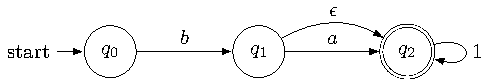
\includegraphics[width=0.7\textwidth]{state_graph}
    \caption{自动机状态转移图}
    \label{fig:state_graph}
\end{figure}

图\ref{fig:state_graph}中,自动机由$q_0$进入,接收字符“b”转移到状态$q_1$,状态$q_1$接收字符“a”转移到状态$q_2$,图中的两个同心圆圈住状态$q_2$表示结束状态( final state )或者接受状态( accepted state ),意味自动机处理字符串到达此状态时,自动机就接受当前处理的字符串,状态$q_2$上有一个指向自己的箭头,意为接收字符“1”之后,仍然指向自己。而状态$q_1$经过$\epsilon$转移到状态$q_2$,意为状态$q_1$可以不接收任何字符即可转移到状态$q_2$。%图\ref{fig:state_graph}中的自动机接受的字符串为$\mathcal{L}=ba(1)^*\cup b(1)^*$。

\begin{definition}[有限自动机 \cite{watson1993taxonomyb}]
    有限自动机(Finite Automata,FA)是一个6元组$(Q,V,T,E,S,F)$,其中
    \begin{itemize}
        \item $Q$ 是有限状态集;
        \item $V$ 是一个字母表;
        \item $ T \in \mathcal{P}(P\times V \times Q) $是一个转移关系;
        \item $ E \in \mathcal{P}(Q\times Q)$ 是一个$\epsilon$-转移关系(空转移,不需要接收字符即可转移);
        \item $ S \subseteq Q $是开始状态集;
        \item $ F \subseteq Q $是结束状态集;
    \end{itemize}
    字母表和函数$\mathcal{P}$的定义分别在“定义\ref{def:Alphabat}” 和 “定义 \ref{pro:mathP}”。
\end{definition}

\begin{example}
    我们可以用$M=(\{q_0,q_1,q_2\},\{b,a,1,\epsilon\},T,E,\{q_0\},\{q_2\})$来指代图\ref{fig:state_graph}中的自动机。其中,$T=\{(q_0 \times b \times q_1),(q_1\times a \times q_2),(q_2\times 1 \times q_2)\}$,$E=(q_1 \times q_2)$。
\end{example}

\begin{remark}
    为了在某些情况下方便的展示状态之间的关系,也把状态转移图写成表格\cite{book1},如图\ref{fig:state_graph}中的自动机,写成表 \ref{tab:sample}:
\begin{table}[!htbp]
    \caption{状态转移函数}
    \label{tab:sample}
    \centering
    \small% fontsize
    \setlength{\tabcolsep}{6pt}% column separation
    \renewcommand{\arraystretch}{1.2}%row space 
    % \begin{tabular}{l p{4em}<{\centering} p{2em}<{\centering} p{2em}<{\centering} p{2em}<{\centering} p{2em}<{\centering}} 
    \begin{tabular}{lccccc}
        \toprule%\hline 
        \multirow{2}{*}{状态说明} & \multirow{2}{*}{状态} & \multicolumn{4}{c}{输入字符} \\
		\cline{3-6}      &    & $a$ & $b$ & $1$ & ${\epsilon}$ \\
        %                        &        & \multicolumn{4}{c}{输入字符} \\
        %\cline{3-6}  {状态说明}  & {状态} &$a$ & $b$ & $1$ & $\epsilon$ \\
        \midrule%\hline
        开始状态(start)  & $q_0$ & -     & $q_1$  &      - &     -    \\
                        & $q_1$ & $q_2$ &    -   &    -   &    $q_2$ \\
        结束状态(final) & $q_2$ &   -   & -      & $q_2$  &    -     \\
        \bottomrule%\hline 
    \end{tabular}
\end{table}
\end{remark}


%\newpage
表格\ref{tab:sample}的状态之间的关系与$T=\{(q_0 \times b \times q_1),(q_1\times a \times q_2),(q_2\times 1 \times q_2)\}$,$E=(q_1 \times q_2)$一一对应,“\mbox{-}” 表示没有相应的转移关系。%%下文中将表格\ref{tab:sample}简称为转移函数。

\begin{remark}[转移关系的表示]
    为了更加简洁的描述转移关系,用 “$T=(q_0 \times b \times q_1)$” 来代表图 \ref{fig:state_graph} 中的 “状态 $q_0$ 接收字符 ‘b’ 转移到状态 $q_1$”。
\end{remark}

\begin{remark}
    本文在不同情况下使用不同的形式来表示转移关系,比如,对于转移关系 $T=(q_0 \times b \times q_1)$ ,也写成 $ q_1 = T(q_0 , b) $。对于图 \ref{fig:state_graph} 中状态 $q_0$ 和 $q_2$ 之间的转移关系,可以描述为 $T(q_0\times w \times q_2)$ 或者 $q_2=T(q_0 , w)$,其中,$w=ba$ 或 $w=b\epsilon$。
\end{remark}

\subsection{有限自动机的性质}

本小节定义有限自动机(Finite automata,下称 FA)的性质,为了使定义更加简洁,引进三个特殊的 FA: $M=(Q,V,T,E,S,F)$ , $M_0=(Q_0,V_0,T_0,E_0,S_0,F_0)$ , $ M_1=(Q_1,V_1,T_1,E_1,S_1,F_1) $。

\begin{definition}[FA 的大小]
    定义一个FA的大小为$|M|=|Q|$。
\end{definition}

\begin{definition}[FA 的同构$\cong$]\label{def:isom}
    我们把同构定义为FA的等价关系。当且仅当 $V_0=V_1$,并且存在双射$g\in Q_0 \longrightarrow Q_1$ ,使得
\begin{itemize}
    \item $T_1 = \{ (g(p,q),a,g(q)) : (p,a,q) \in T_0 \}$
    \item $E_1 = \{ (g(p,q),a,g(q)) : (p,q) \in E_0\}$
    \item $S_1 = \{ g(s):s\in S_0 \}$
    \item $F_1 = \{ g(f):f\in F_0 \}$
\end{itemize}
时$M_0$和$M_1$是同构的(写作$M_0 \cong M_1$)。
\end{definition}

\begin{definition}[转移关系 $T$ 的扩展]
    我们把$T \in V \longrightarrow \mathcal{P} (Q \times Q) $ 到 $ T^* \in V^* \longrightarrow \mathcal{P} (Q \times Q)  $的转换关系以如下方式扩展: 
    \[ 
        T^*(\epsilon) = E^* 
    \]
    且对于$(a\in V,w\in V^*)$ 有 
    \[ 
        T^*(aw) = E^* \circ T(a) \circ T^*(w)    
    \]
    操作符$\circ$在定义 2.5 中定义。
\end{definition}

\begin{definition}[左语言和右语言 \cite{watson1993taxonomyb}]
    状态($M$中)的左语言由函数$ \overleftarrow{\mathcal{L}} _M \in Q \longrightarrow \mathcal{P}(V^*)$ 给出,其中:
    \[ 
        \overleftarrow{\mathcal{L}}_M (q) = ( \cup s:s \in S : T^*(s,q) )  
    \] 
    状态($M$中)的右语言由函数$ \overrightarrow{\mathcal{L}} _M \in Q \longrightarrow \mathcal{P}(V^*)$给出,其中 
    \[ 
        \overrightarrow{\mathcal{L}}_M (q) = ( \cup f:f \in F : T^*(q,f) ) 
    \] 
    通常在没有歧义的时候移除下标$M$。
\end{definition}

\begin{definition}[ FA 的语言 \cite{watson1993taxonomyb}]
    有限自动机的语言由函数 $\mathcal{L}_{FA} \in FA \longrightarrow \mathcal{P}(V^*) $给出,该函数的定义为式 \ref{eq:languageoffa}: 
    \begin{equation}\label{eq:languageoffa}
        \mathcal{L}_{FA} (M) = (\cup s,f:s \in S \land f \in F : T^* (s,f))
    \end{equation}
\end{definition}

\begin{example}[FA 的语言]
    图 \ref{fig:state_graph} 中的 FA 接受的语言为 $ \mathcal{L}= \{ ba(1)^*\cup b(1)^* \}$。下文中使用符号 $\mathcal{L}$ 代替 FA 接受的 “语言”。
\end{example}

\begin{definition}[完全 FA ($Complete$)\cite{watson1993taxonomyb}]\label{def:complete}
    一个完全 FA 满足式 (\ref{eq:complete} ):
    \begin{equation} \label{eq:complete}
        Complete(M) \equiv ( \forall q,a:q\in Q \land a \in V : T(q,a) \not= \emptyset ) 
    \end{equation}
\end{definition}

\begin{definition}[$\epsilon$-$free$]
    当且仅当 $E=\emptyset$时,$M$ 是 $\epsilon$-$free$ 的。
\end{definition}

\begin{definition}[可达状态 \cite{watson1993taxonomya}]\label{def:rechable-state}
    可达状态分为 “开始可达状态” 和 “可达结束状态” ( $M$ 中),其中
    \begin{itemize}
        \item 开始可达状态:从开始状态可以到达的状态,写作 $SReachable(M)$;
        \item 可达结束状态: 能到达结束状态的状态,写作 $FReachable(M)$;
    \end{itemize}
    可达状态定义为:
    \[ Reachable(M) = SReachable(M) \cap FReachable(M) \]
\end{definition}

\begin{definition}[Start-useful 自动机\cite{watson1993taxonomyb}]
    一个 $Useful_s$ 自动机 定义如下: 
    \[ Useful_s (M) \equiv ( \forall q:q \in Q : \overleftarrow{\mathcal{L}} (q) \not= \emptyset ) \]
\end{definition}

\begin{definition}[Final-useful 自动机\cite{watson1993taxonomyb}]
    一个 $Useful_f$ 自动机 定义如下: 
    \[ Useful_f (M) \equiv ( \forall q:q \in Q : \overrightarrow{\mathcal{L}} (q) \not= \emptyset ) \]
\end{definition}

\begin{definition}[Useful 自动机\cite{watson1993taxonomyb}]
    $Useful$ 自动机是一个只有可达状态的 FA:
    \[ Useful (M) \equiv Useful_s (M) \land Useful_f (M) \]
\end{definition}

\begin{example}
    如图 \ref{fig:UsefulFA} 所示,其中
    \begin{itemize}
        \item 图 \ref{fig:UsefulFA-2} 为一个 $Useful$ FA;
        \item 图 \ref{fig:UsefulFA-1} 中状态 $q_1$ 不是一个开始可达状态,也称开始不可达状态(start-unreachable);
        \item 图 \ref{fig:UsefulFA-1} 中状态 $q_2$ 不是一个可达结束状态,也称陷阱状态(final-unreachable)\cite{book1}。
    \end{itemize}
\end{example}

\begin{figure}[!htbp]
    \centering
    \begin{subfigure}[b]{0.45\textwidth}
        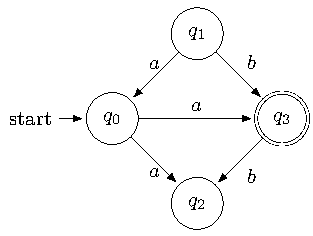
\includegraphics[width=\textwidth]{UsefulFA-1}
        \caption{}
        \label{fig:UsefulFA-1}
    \end{subfigure}
    ~
    \begin{subfigure}[b]{0.45\textwidth}
        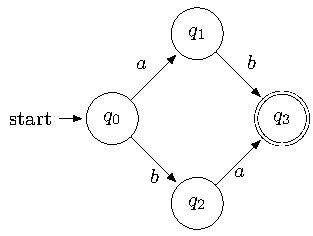
\includegraphics[width=\textwidth]{UsefulFA-2}
        \caption{}
        \label{fig:UsefulFA-2}
    \end{subfigure}
    \caption{}
    \label{fig:UsefulFA}
\end{figure}

\begin{definition}[确定的有限自动机 \cite{watson1993taxonomyb}]
    当且仅当 
    \begin{itemize}
        \item 无多重开始状态;
        \item 无$\epsilon$转移关系;
        \item 转移函数$T \in Q \times V \longrightarrow \mathcal{P} (Q) $ 不将 $Q \times V$ 映射至多个状态。
    \end{itemize}
    时有限自动机$M$是确定的,称 $M$ 为确定的有限自动机(Deterministic Finite Automata,下称 DFA)。
    公式形式表达为式 \ref{eq:DetFA} :
    \begin{equation}\label{eq:DetFA}
    Det(M) \equiv ( |S| \leq 1 \land \epsilon\mbox{-} free(E) \land ( \forall q,a:q \in Q \land a \in V : |T(q,a)| \leq 1 )) 
    \end{equation}
    且有$ DFA \subseteq FA$。
\end{definition}


\begin{definition}[DFA 的最小化\cite{watson1993taxonomyb}]\label{def:min}
    满足以下条件时,$M\in DFA$是最小的:
    { \small \[  Min(M) \equiv (\forall M' : M' \in DFA \land Complete(M') \land \mathcal{L}(M) = \mathcal{L}_{FA}(M') : |M| \leq |M'| ) \] }
函数 $Min$ 仅定义在 DFA 上。一个最小的但是仍然完全的 DFA 的定义如下:
{\small \[  Min_{\mathcal{C}}(M) \equiv ( \forall M':M' \in DFA \land Complete(M') \land \mathcal{L}_{FA}(M) = \mathcal{L}_{FA}(M'): |M| \leq |M'| ) \] }
$Min_{\mathcal{C}}$ 仅定义在完全 DFA 上。
\end{definition}

\subsection{有限自动机的变换}

\begin{transformation}[FA 的反转(reversal)\cite{watson1993taxonomyb}]\label{trans:reverse}
        $FA$反转由上标函数$ R \in FA \to FA $ 给出,它的定义如下:
        \[ (Q,V,T,S,F)^R = (Q,V,T^R,E^R,F,S) \]
    函数 $R$ 满足
    \[ (\forall M : M \in FA : ( \mathcal{L}_{FA} (M) )^R = \mathcal{L}_{FA}(M^R)) \]
\end{transformation}

\begin{transformation}[移除开始状态不可达状态\cite{watson1993taxonomyb}]\label{trans:usefuls}
    变换$useful_s \in FA \longrightarrow FA$移除开始状态不可达状态:
    \begin{table}[!htbp]
        \centering
        %\small% fontsize
        \setlength{\tabcolsep}{1pt}% column separation
        \renewcommand{\arraystretch}{1.3}%row space 
        \begin{tabular}{lcll} 
            $useful_s(Q,V,T,E,S,F)$ & = & {\bfseries let} & $U = SReachable(Q,V,T,E,S,F)$ \\
                                    &   & {\bfseries in}  &                               \\
                                    &   &                 & $(U,V,T \cap (U\times V \times U), E \cap (U \times U), S \cap U, F \cap U )$  \\
                                    &   & {\bfseries end} &                               \\
        \end{tabular}
    \end{table}
% \\除了性质 $ \mathcal{L}_{FA}(subset(M))= \mathcal{L}_{FA}(M) $(对所有的$M \in FA$)之外,
 \\ 函数 $ useful_s $ 满足
\[  (\forall M : M \in FA : Useful_s ( useful_s(M) ) \land \mathcal{L}_{FA} (useful_s(M)) = \mathcal{L}_{FA}(M)) \]
\end{transformation}

% \begin{transformation}[子集构造\cite{watson1993taxonomyb}]
%     函数$subset$把一个$\epsilon$-$free$ FA 转换为一个 DFA (在子句 \textbf{let} $T'\in \mathcal{P}(Q) \times V \longrightarrow \mathcal{P}(\mathcal{P} (Q) )$ 中): 
%     \begin{table}[!htbp]
%         \centering
%         %\small% fontsize
%         \setlength{\tabcolsep}{4pt}% column separation
%         \renewcommand{\arraystretch}{1.4}%row space 
%         \begin{tabular}{lcll} 
%             $subset(Q,V,T,\emptyset,S,F)$ & = & {\bfseries let} & $T'(U,a) = \{ (q:q\in U : T(q,a) ) \} $ \\
%                                           &   &                 & $F'= \{ U : U \in \mathcal{P}(Q) \land U \cap F \not= \emptyset \} $ \\
%                                           &   & {\bfseries in}  &                                         \\
%                                           &   &                 & $ ( \mathcal{P}(Q),V,T',\emptyset,\{ S \},F' ) $  \\
%                                           &   & {\bfseries end} &                               \\
%         \end{tabular}
%     \end{table}
%     \\除了性质 $ \mathcal{L}_{FA}(subset(M))= \mathcal{L}_{FA}(M) $(对所有的$M \in FA$)之外,函数 $subset$ 还满足
%     \[ (\forall M : M \in FA \land \epsilon \mbox{-} free(M) : Det(subset(M)) \land Complete(subset(M))) \]
%     有时候也把它说成“幂集”构造。
% \end{transformation}

\begin{definition}[优化的子集构造\cite{watson1993taxonomyb}]
    函数$subsetopt$把一个$\epsilon$-$free$ $FA$ 转换为一个 DFA。%此函数是$subset$的一个优化版本:
    \begin{table}[!htbp]
        \centering
        %\small% fontsize
        \setlength{\tabcolsep}{2pt}% column separation
        \renewcommand{\arraystretch}{1.3}%row space 
        \begin{tabular}{lcll} 
            $subsetopt(Q,V,T,\emptyset,S,F)$ & = & {\bfseries let} & $ T'(U,a) = \{ (q:q\in U : T(q,a) ) \} $ \\
                                          &   &                 & $ Q' = \mathcal{P} (Q) \setminus \{ \emptyset \} $ \\
                                          &   &                 & $ F'= \{ U : U \in \mathcal{P}(Q) \land U \cap F \not= \emptyset \} $ \\
                                          &   & {\bfseries in}  &                                         \\
                                          &   &                 & $ ( Q',V,T' \cap (Q' \times V \times Q'),\emptyset,\{ S \},F' ) $  \\
                                          &   & {\bfseries end} &                               \\
        \end{tabular}
    \end{table}
    \\除了性质$\mathcal{L}_{FA} (subsetopt(M)) = \mathcal{{L}} (M) $(对所有的$M\in FA$)之外,函数$subsetopt$还满足
    $$ ( \forall M : M \in FA \land \epsilon \mbox{-}free(M) : Det(subset(M)) )  $$
\end{definition}

\section{等价性和最小化}

令 $M=\{Q,V,T,\emptyset,S,F \}$ 为一个完全 DFA,并且 $M$ 中所有状态都是可达状态。

\begin{definition}[状态的等价\cite{watson1993taxonomyb}]
    当$M$ 中的状态 $ p,q $ 满足式 (\ref{eq:equivalence}) 时,称状态 $p,q$ 等价。
    \begin{equation} \label{eq:equivalence}
        (p,q) \in E \equiv ( \overrightarrow{\mathcal{L}}(p) = \overrightarrow{\mathcal{L}}(q) )
    \end{equation}
    其中,$E$ 为等价关系(Equivalence)。
\end{definition}

\begin{definition}[状态的等价\cite{book1}]
    给出状态等价的另一种描述。对给定的 $DFA$ $M=(Q,V,T,\emptyset,S,F)$,如果 $\exists w \in V^*$ ,使得$Q$ 中的两个状态 $p$ 和 $q$,若$T(q,w)\in F$ 和 $T(p,w)\in F$ 有且仅有一个成立,那么称 $p$ 和 $q$ 是可区分的,否则称 $p$ 和 $q$ 等价,写作 $p \equiv q$。
\end{definition}

\begin{remark}
    关系 $D$ (Distinguishable) 是可区分的状态,$E$ 和 $D$ 满足 $D=\lnot E$。
\end{remark}

\begin{remark}[操作符 $\setminus$]
    $M$ 中,若 $p \in (Q \setminus F)$ , 那么 $ p \notin F$。
\end{remark}

\begin{remark}
    $\forall p,q: p \in (Q \setminus F) \land q \in F$,有 $ p \not\equiv q $。
\end{remark}

\subsection{最小化}

最小化是对于一个给定的 DFA $M$,找到一个与 $M$ 接受同样的 $\mathcal{L}$ 的且状态数最少的 DFA $M_1$ ($|M_1|\leq |M|$)的过程, 最小化算法用来计算 DFA 中的关系 $D$ 和关系 $E$,只需计算其中一个即可得到 $M_1$ \cite{watson1993taxonomyb}(本文仅针对 DFA 应用最小化算法)。

给出一种用于 DFA 的最小化算法\cite{book1,zf14Min,yingjie2009describing},描述如算法 \ref{ali:classic-al} 所示:

\begin{algorithm}
    \caption{经典算法(也称标记法\cite{zf14Min})}\label{ali:classic-al}
    \begin{algorithmic}[1]
        \Require DFA $M$
        \Ensure 与 $M$ 同构的最小的 DFA
        \Statex
        \State $ \forall (p,q) \in (Q \setminus F) \times F $,标记状态对 $(p,q)$ 
        \Repeat
            \ForAll {未被标记的状态对$(p,q)$ }
                \ForAll {$\forall x \in V$}
                    \If {状态对$ (T(p,x),T(q,x)) $ 被标记了}
                        \State 标记状态对$(p,q)$
                    \EndIf
                \EndFor
            \EndFor
        \Until{没有新的状态对被标记}
    \end{algorithmic}
\end{algorithm}

\begin{theorem}
    算法 \ref{ali:classic-al} 的时间复杂度为 $\mathcal{O}(n^2)$ \cite{yingjie2009describing}。
\end{theorem}

\begin{theorem}
    算法 \ref{ali:classic-al} 移除不可达状态后的 DFA 为最小的 DFA \cite{book1}。
\end{theorem}

% \begin{enumerate}[1.]
%     \item $ \forall (p,q) \in (Q \setminus F) \times F $,标记可区分状态表中的表项 $(p,q)$ 
%     \item $ \forall (p,q) \in (Q \setminus F) \times \in (Q \setminus F) \cup F \times F \land p \not =  q $ ,进行以下步骤:
%     \item 如果 $\exists a \in V $,若可区分状态表项 $(T(p,a),T(q,a))$ 已经被标记,那么继续标记可区分状态表 $(p,q)$;
%     \item 递归重复步骤 2 ,步骤 3 ;
%     \item 否则 $\forall a \in V $,如果 $T(p,a) \not= T(q,a) $ 且 $(p,a)$ 与  $(T(p,a),T(q,a))$ 不是同一个状态对,那么将 $(p,q)$ 放在  $(T(p,a),T(q,a))$ 的关联表上。
% \end{enumerate}

% \begin{remark}
%     本文把等价状态的集合叫做等价类。
% \end{remark}
% 其中
% \begin{itemize}
%     \item 可区分状态表,用来标记状态对是否可以被区分。如果相应的表项可以被区分,则使用 $\checkmark$ 标示。
%     \item 状态关联表。
% \end{itemize}

\begin{example}
    使用算法 \ref{ali:classic-al} 对图 \ref{fig:DFAMin-3-0-minexample} 中的 DFA 进行最小化。
\end{example}

\begin{figure}[!htbp]
    \centering
    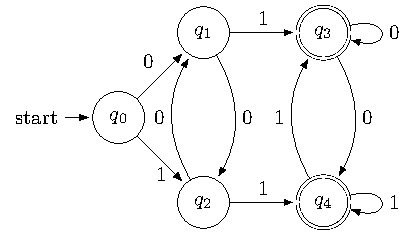
\includegraphics[width=0.6\textwidth]{Min/markAlexample}
    \caption{一个接受 $\mathcal{L}=\{ 0(0)^*1(0|1)^* \cup 1(0)^*1(0|1)^*  \}$ 的 DFA }
    \label{fig:DFAMin-3-0-minexample}
\end{figure}


\begin{enumerate}[(1)]
    \item 首先标记状态对$(q_0,q_3)$,$(q_0,q_4)$,$(q_1,q_3)$,$(q_1,q_4)$,$(q_2,q_3)$,$(q_2,q_4)$。剩下需要计算的状态对为$(q_0,q_1)$,$(q_0,q_2)$,$(q_1,q_2)$,$(q_3,q_4)$;
    \item 对于状态对$(q_0,q_1)$,$T(q_0,0)=q_1$,$T(q_1,0)=q_2$,此时状态对$(q_1,q_2)$未被标记,无操作;再看$T(q_0,1)=q_2$,$T(q_1,1)=q_3$,此时$(q_0,q_3)$已经被标记,那么标记状态对$(q_0,q_1)$;
    \item 对于状态对$(q_0,q_2)$,$T(q_0,0)=q_1$,$T(q_2,0)=q_1$,不做处理,再看$T(q_0,1)=q_2$,$T(q_2,1)=q_4$,此时状态对$(q_0,q_4)$已经被标记,那么标记$(q_0,q_2)$;
    \item 对于状态对$(q_1,q_2)$,$T(q_1,0)=q_2$,$T(q_2,0)=q_1$,不做处理,再看$T(q_1,1)=q_3$,$T(q_2,1)=q_4$,此时状态对$(q_3,q_4)$未被标记,无操作;
    \item 对于状态对$(q_3,q_4)$,$T(q_3,0)=q_3$,$T(q_4,0)=q_3$,不做处理,再看$T(q_3,1)=q_4$,$T(q_4,1)=q_4$,不做处理;
    \item 第一次迭代结束,此时还有状态对$(q_1,q_2)$和$(q_3,q_4)$未被标记。
    \item 对于状态对$(q_1,q_2)$,根据第(4)步,算法无操作;
    \item 对于状态对$(q_3,q_4)$,根据第(5)步,算法无操作;
    \item 本次迭代未标记任何状态对,算法结束,此时还有状态对$(q_1,q_2)$和$(q_3,q_4)$未被标记。
\end{enumerate}

算法结束后还有状态对$(q_1,q_2)$和$(q_3,q_4)$未被标记,也就是说$q_1 \equiv q_2$,$q_3 \equiv q_4$。此时的 DFA 为图 \ref{fig:DFAMin-3-0-minexample-rel}。

\begin{figure}[!htbp]
    \centering
    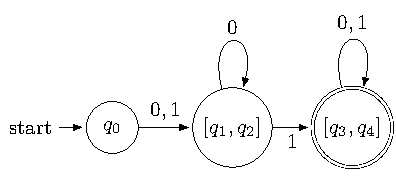
\includegraphics[width=0.5\textwidth]{Min/markAlexample-rel}
    \caption{与图 \ref{fig:DFAMin-3-0-minexample} 同构的最小的 DFA }
    \label{fig:DFAMin-3-0-minexample-rel}
\end{figure}


\chapter{等价关系和最小化}

% {\heiti 这是一段黑体字}

% {\rmfamily rmfamily}

% {\ttfamily ttfamily 1234567890 ABCDEFGQWE}

% {\fangsong 普通仿宋字体}

% {\fangsong\bfseries 加粗仿宋字体}

% Xidian University

% \begin{table}[!htbp]
%     \caption{状态转移函数}
%     \label{tab:sample2}
%     \centering
%     \small% fontsize
%     \setlength{\tabcolsep}{4pt}% column separation
%     \renewcommand{\arraystretch}{1.2}%row space 
%     \begin{tabular}{l|c|c|c|c|c} 
%         \hline
%         参数 & 条件 & Min & Typ & Max & 单位 \\
%         \hline
%         \multicolumn{6}{l}{湿度} \\
%         \hline
%         \multirow{2}{*}{分辨率} & \multirow{2}{*}{ } & 1 & 1 & 1 & RH \\

%         \cline{3-6}            &                    &   & 16 &  &  Bit \\
%         \hline
%     \end{tabular}
% \end{table}

% \begin{algorithm}
%     \caption{Euclid’s algorithm}\label{euclid}
%     \begin{algorithmic}[1]
%         \Procedure{Euclid}{$a,b$}\Comment{The g.c.d. of a and b}
%         \State $r\gets a\bmod b$
%         \While{$r\not=0$}\Comment{We have the answer if r is 0}
%         \State $a\gets b$
%         \State $b\gets r$
%         \State $r\gets a\bmod b$
%         \EndWhile\label{euclidendwhile}
%         \State \textbf{return} $b$\Comment{The gcd is b}
%         \EndProcedure
%         \do $L \not= \emptyset \longrightarrow $ 
        
%     \end{algorithmic}
% \end{algorithm}

% \mbox{ } $P:=[Q]_{E_0}$; \\
% \mbox{ } $L:= ( \mbox{\textbf{if }} ( |F| \leq |Q \setminus F | ) \mbox{\textbf{then }} \{F\} \mbox{\textbf{else }} \{ Q \setminus F \} \mbox{\textbf{fi }} ) \times V $; \\
% \mbox{ } $ \{ \mbox{恒有: } [Q]_E \sqsubseteq P \sqsubseteq [Q]_{E_0} \land L \subseteq (P \times V) $ \\
% \mbox{   } $ \land (\forall Q_0,Q_1,a:Q_0 \in Q \land (Q_1,a) \in L : \neg Splittable (Q_0,Q_1,a)) \Rightarrow (P=[Q]_E) \} $ \\
% \mbox{ } $ \mbox{\textbf{do }} L \not= \emptyset \longrightarrow $ \\ 
% \mbox{   } $ \mbox{\textbf{let }} Q_1,a:(Q_1,a) \in L $; \\
% \mbox{   } $ P_{old} := P $; \\
% \mbox{   } $ L := L \setminus \{ (Q_1,a) \} $; \\
% \mbox{   } $ \{  \mbox{恒有: } [Q]_E \sqsubseteq P \sqsubseteq P_{old} \} $ \\
% \mbox{   } $ \mbox{\textbf{for }} Q_0 : Q_0 \in P_{old} \land Splittable (Q_0,Q_1,a) \mbox{\textbf{ do }} $ \\
% \mbox{     } $ Q'_0 := \{ p:p \in Q_0 \land T(p,a) \in Q_1 \} $; \\
% \mbox{     } $ P:= P \setminus \{ Q_0 \} \cup \{ Q_0 \setminus Q'_0,b \} $;\\
% \mbox{     } $ \mbox{\textbf{for }} b:b \in V \mbox{\textbf{ do }} $ \\
% \mbox{       } $ \mbox{\textbf{if }} (Q_0,b) \in L \rightarrow L := L \setminus \{ (Q_0,b) \} \cup \{ (Q'_0,b),(Q_0, \setminus Q'_0,b ) \} $;\\ 
% \mbox{       } $ \talloblong (Q_0,b) \notin L \rightarrow $ \\
% \mbox{         } $ L := L \cup (\mbox{\bfseries if} ( |Q'_0| \leq |Q_0 \setminus Q'_0| ) \mbox{\bfseries then} \{ (Q'_0 , b) \} \mbox{\bfseries else} \{ ( Q'_0 \setminus Q'_0,b ) \} \mbox{\bfseries fi} ) $ \\
% \mbox{       } $ \mbox{\textbf{fi}} $ \\
% \mbox{     } $ \mbox{\textbf{rof}} $ \\
% \mbox{   } $ \mbox{\textbf{rof}} $ \\
% \mbox{   } $ \{ (\forall Q_0,Q_0 \in P : \neg Splittable(Q_0,Q_1,a)) \} $ \\
% \mbox{ } $ \mbox{\textbf{od }} \{ P = [Q]_E \} $ \\

% \begin{algorithm}
%     \caption{Euclid’s algorithm}\label{euclid}
%     \begin{program}
%         $P:=[Q]_{E_0}$;
%         $L:= ( \mbox{\textbf{if }} ( |F| \leq |Q \setminus F | ) \mbox{\textbf{then }} \{F\} \mbox{\textbf{else }} \{ Q \setminus F \} \mbox{\textbf{fi }} ) \times V $;
%     \end{program}
% \end{algorithm}

\section{等价关系}

等价关系是进行 DFA 最小化的基础,本节定义状态的等价及一些应用。
\chapter{实例化类DFA对象}

\section{DFA类}
在本文中,我们仅仅对 DFA 应用最小化算法,FIRE engine 中的DFA类为应用最小化算法的类。
FIRE engine 提供了多种方式构造一个 DFA,类 DFA 的部分实现如表 \ref{tab:Class-DFA} 
% \lstset{style=mystyle}
% \begin{lstlisting}[language=C++,label={lst:consDFA},caption={class DFA}]
% class DFA : virtual public FAabs
% {
% public:
%     // Default copy constructor, destructor, operator= are okay.
%     inline DFA();

%     // A special constructor used for subset construction etc.
%     inline DFA(const DFA_components& r);
%     ……
%     StatePool Q;
%     // S must be a singleton set, or empty. |S| <= 1
%     StateSet S;
%     StateSet F;  // final states
%     DTransRel T;
% }
% ……
% inline DFA::DFA(const DFA_components& r) :Q(r.Q), S(r.S), F(r.F), T(r.T)
% {
%     current = Invalid;
%     assert(class_invariant());
% }
% ……
% \end{lstlisting}

\begin{table}[!htbp]
    \caption{类 DFA}
    \label{tab:Class-DFA}
    \centering
    \small% fontsize
    \setlength{\tabcolsep}{4pt}% column separation
    \renewcommand{\arraystretch}{1.2}%row space 
    %\begin{tabular}{lcrr} 
        \begin{tabular}{llll} %l p{4em}<{\centering} p{3em}<{\centering} p{3em}<{\centering}
        \toprule 
         \multicolumn{4}{c}{Class DFA} \\
        \midrule
        名称& 类型 & 属性  &\mbox{说明} \\
        \midrule
        Q & StatePool & protected &          \\
        S & StateSet  & protected &  $S\in Q$ \\
        F & StateSet  & protected &  $F\in Q$\\
        T & DTransRel & protected &  转移关系\\
        \midrule 
        DFA(const DFA\_components\& r);& & public &构造函数 \\
        reconstruct(const DFA\_components\& r); & DFA\& & public & \\
        determinism() const; & DFA & public & \\
        reverse(); & DFA\& & public & 反转 DFA \\
        min\_Brzozowski(); & DFA\& & public & 最小化算法 \\
        min\_HopcroftUllman(); & DFA\& & public & 最小化算法 \\
        min\_dragon(); & DFA\& & public & 最小化算法 \\
        min\_Hopcroft(); & DFA\& & public & 最小化算法 \\
        min\_Watson(); & DFA\& & public & 最小化算法 \\
        usefulf(); & DFA\& & public &  \\
        split(State,State,CharRange,StateEqRel\&); & State & public & 分割等价类 \\
        \bottomrule 
    \end{tabular}
\end{table}


由表 \ref{tab:Class-DFA} 可知,类$DFA$默认情况下,提供一个用“DFA\_com-ponents”变量的引用来实例化DFA对象的方法。

除了使用“DFA\_components”来实例化DFA对象之外,FIRE engine 还可以通过执行类 LBFA 的成员函数 LBFA::determinism() 来将 LBFA 对象转化成一个 DFA 对象,拥有同样功能的类还有类 FA 、类 RFA 和类 RBFA ,这四个类与类 DFA 都继承自类 FAabs 。

类 FAabs 及其派生类关系如图\ref{fig:FAabsRel}

\begin{figure}[!htbp]
    \centering
    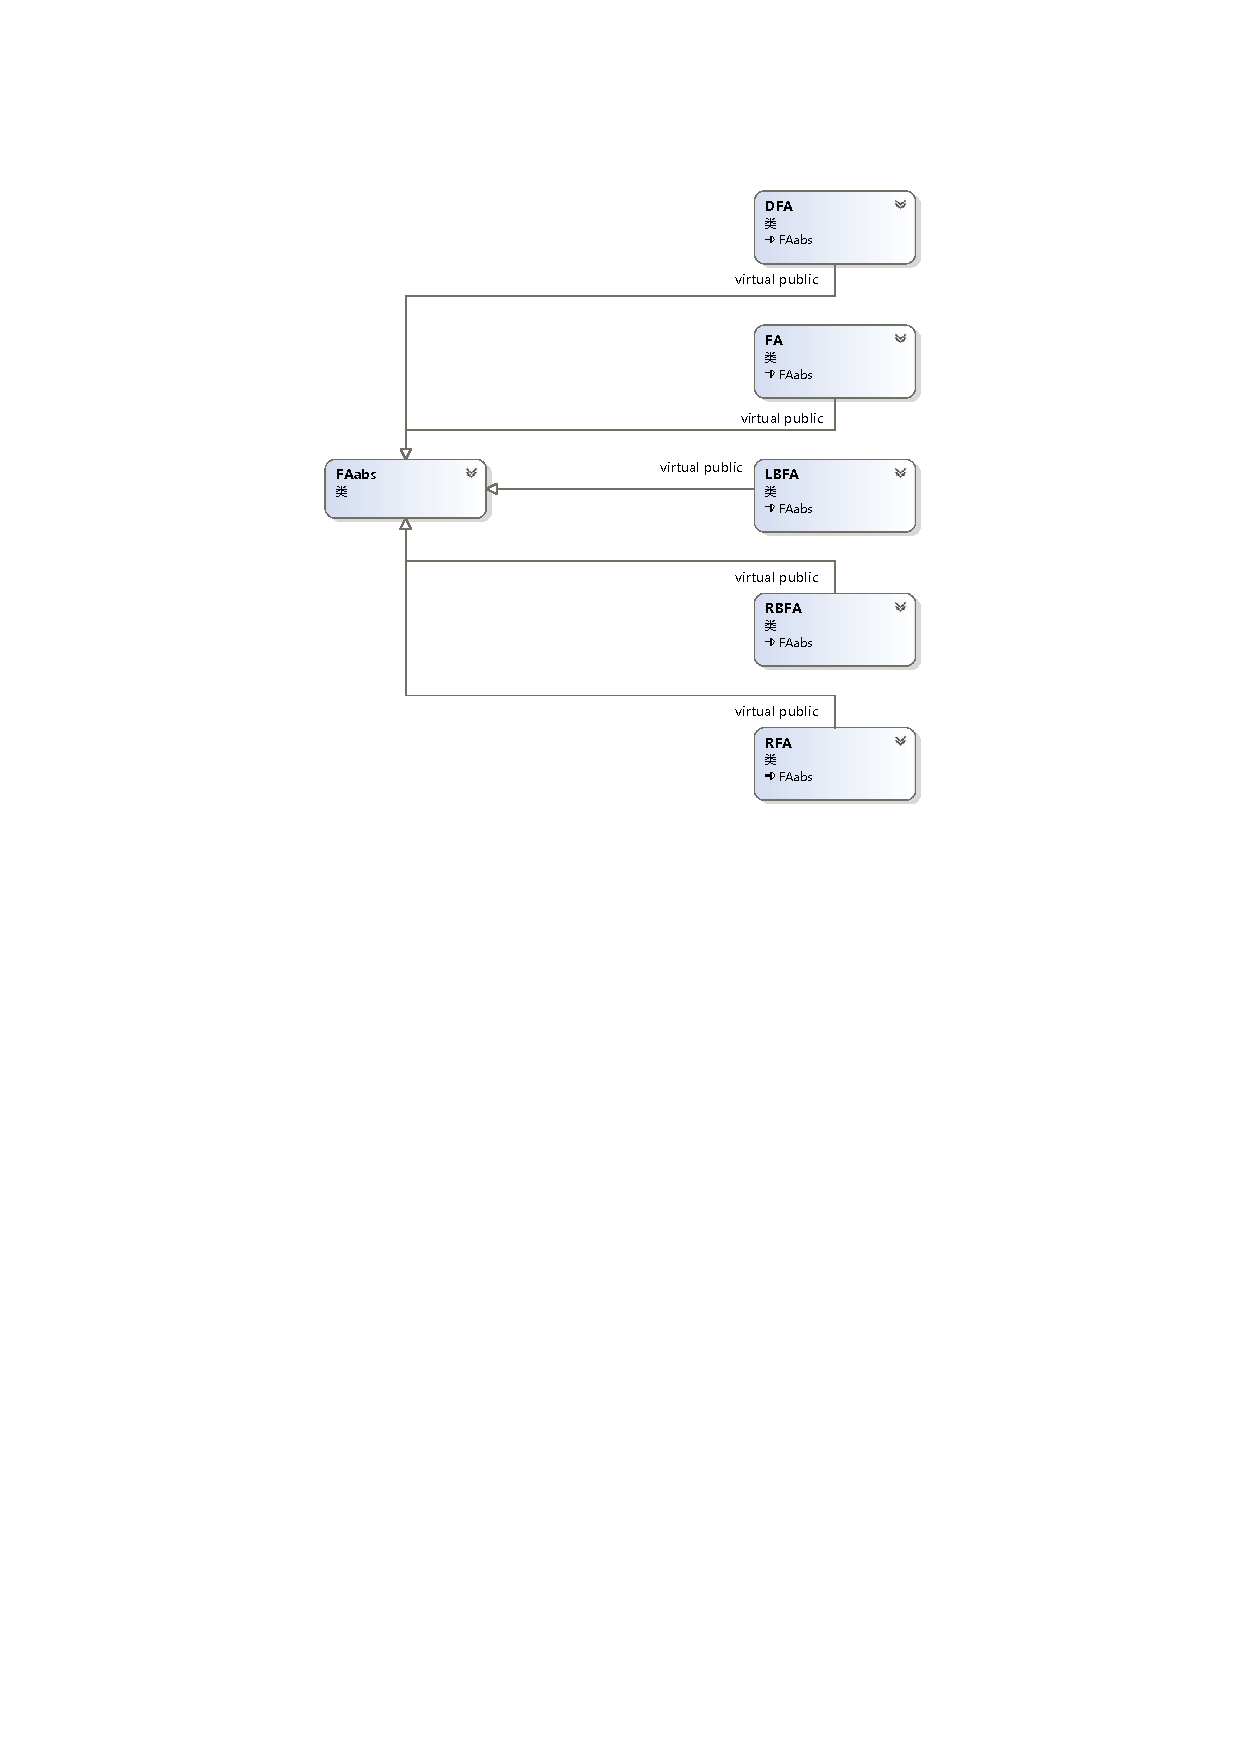
\includegraphics[width=0.7\textwidth]{FAabsRel}
    \caption{类FAabs及其派生类}
    \label{fig:FAabsRel}
\end{figure}

%\newpage
\section{DFA\_components 结构体}\label{sc:dfa_com}% ~\label{sc:dfa_com}

从“DFA\_components”构造一个$DFA$对象是最简单直接的方法,观察“DFA\_components”的实现,如表\ref{tab:DFA-components}所示
\begin{table}[!htbp]
    \caption{DFA\_components}
    \label{tab:DFA-components}
    \centering
    \small% fontsize
    \setlength{\tabcolsep}{4pt}% column separation
    \renewcommand{\arraystretch}{1.2}%row space 
    %\begin{tabular}{lcrr} 
        \begin{tabular}{p{3em}<{\centering} p{5em}<{\raggedright} p{5em}<{\raggedright}} %l p{4em}<{\centering} p{3em}<{\centering} p{3em}<{\centering}
        \toprule 
         \multicolumn{3}{c}{结构体 DFA\_components} \\
        \midrule
        名称& 类型 & \mbox{说明} \\
        \midrule
        Q & StatePool &           \\
        S & StateSet  &  $S\in Q$ \\
        F & StateSet  &  $F\in Q$ \\
        T & DTransRel &  转移关系  \\
        \bottomrule
    \end{tabular}
\end{table}
由表\ref{tab:DFA-components}可知,结构体 DFA\_components 内包含 StatePool 变量$Q$, StateSet 变量$S$, DTransRel 变量$T$, StateSet 变量$F$。若需要声明一个 DFA\_components 变量,则需要分别实例化 StatePool 、StateSet、DTransRel对象。这几个类还分别继承自其他的类,如图 \ref{fig:DFARel} 所示。

\begin{figure}[!htbp]
    \centering
    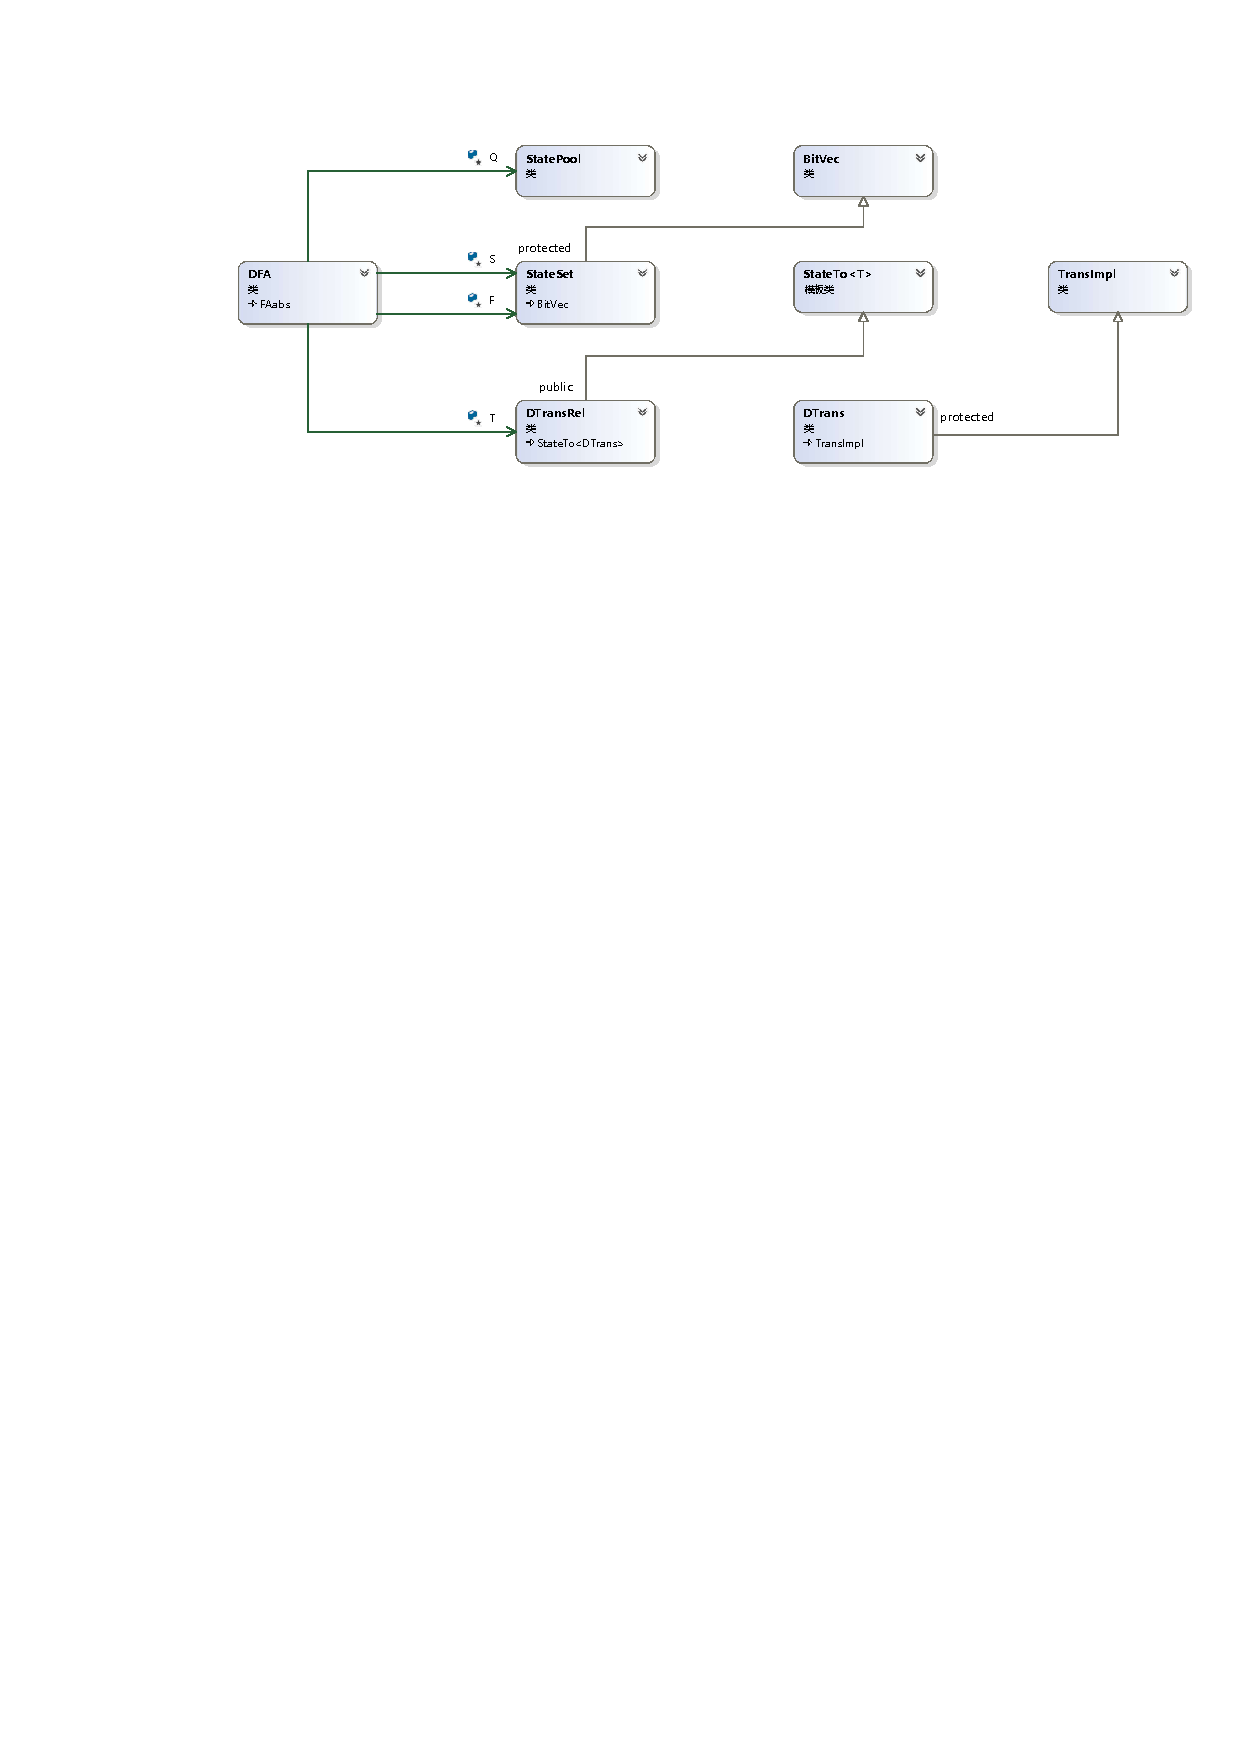
\includegraphics[width=\textwidth]{DFARel}
    \caption{DFA与其成员类及成员类的基类}
    \label{fig:DFARel}
\end{figure}

类 DFA 的成员变量 “T” 为一个 DTransRel 对象,公有继承自模板类 StateTo<T>,模板参数 “T” 为保护继承自类 TransImpl 的类 DTrans 。

\subsection{StatePool 类}
StatePool类的部分实现如表 \ref{tab:Class-StatePool} (文件$StatePool.h$):
% \lstset{style=mystyle}
% \begin{lstlisting}[language=C++,label={lst:StatePool},caption={StatePool}]
% class StatePool
% {
% public:
%     // How many states are already allocated(one more than that last allocated one,
%     // since it begins at 0).
%     inline int size() const;
%     ……
%     // Allocate a new state.
%     inline State allocate();
%     ……
% private:
%     // The next one to be allocated.
%     int next;
% };
% ……
% inline int StatePool::size() const
% {
%     return(next);
% }
% ……
% inline State StatePool::allocate()
% {
%     return(next++);
% }
% \end{lstlisting}

\begin{table}[!htbp]
    \caption{类 StatePool}
    \label{tab:Class-StatePool}
    \centering
    \small% fontsize
    \setlength{\tabcolsep}{4pt}% column separation
    \renewcommand{\arraystretch}{1.2}%row space 
    %\begin{tabular}{lcrr} 
        \begin{tabular}{llll} %l p{4em}<{\centering} p{3em}<{\centering} p{3em}<{\centering}
        \toprule 
         \multicolumn{4}{c}{Class StatePool} \\
        \midrule
        名称& 类型 & 属性  &\mbox{说明} \\
        \midrule
        next & int & private &          \\
        \midrule 
        StatePool(const StatePool\& r);& & public &构造函数 \\
        size() const; & int & public & \\
        allocate();  &   State &  public & \\
        set\_domain(const\ int r); & int & public & \\
        contains(const State r) const; & int & public & \\
        \bottomrule 
    \end{tabular}
\end{table}
如表 \ref{tab:Class-StatePool} 所示,其中 StatePool::size() 和 StatePool::allocate() 为类 StatePool 两个比较重要的函数,前者为自动机 $M$ 的大小,也即 $|M|=|Q|$。 StatePool::allocate() 用来向 StatePool 增加新的状态。
\subsection{StateSet 类}
类$StateSet$的部分声明如表 \ref{tab:Class-StateSet}(文件$StateSet.h$):
% \lstset{style=mystyle}
% \begin{lstlisting}[language=C++,label={lst:StateSet},caption={StateSet}]
% class StateSet :protected BitVec
% {
% public:
% ……
%     // inserts a State. r = [0,domain())
%     inline StateSet& add(const State r);
    
%     // set How many States can this set contain.
%     // [O, r) can be contained in *this.
%     inline void set_domain(const int r);
% ……
% }
% \end{lstlisting}

\begin{table}[!htbp]
    \caption{类 StateSet}
    \label{tab:Class-StateSet}
    \centering
    \small% fontsize
    \setlength{\tabcolsep}{4pt}% column separation
    \renewcommand{\arraystretch}{1.2}%row space 
    %\begin{tabular}{lcrr} 
        \begin{tabular}{llll} %l p{4em}<{\centering} p{3em}<{\centering} p{3em}<{\centering}
        \toprule 
         \multicolumn{4}{c}{Class StateSet : protected BitVec} \\
        \midrule
        名称& 类型 & 属性  &\mbox{说明} \\
        \midrule 
        StateSet(); &  &  public & 构造函数 \\
        empty() const; & int & public & \\
        size() const;  & int & public & \\
        complement();  & StateSet\& & public & 求补集 \\
        add(const State r);  & StateSet\& & public &  \\
        remove(const State r);  & StateSet\& & public &  \\
        set\_union(const StateSet\& r);  & StateSet\& & public & 求并集 \\
        intersection(const StateSet\& r);  & StateSet\& & public & 求交集 \\
        remove(const StateSet\& r);  & StateSet\& & public &  \\
        smallest() const; & State & public & \\
        set\_domain(const int r); & void & public & \\
        \bottomrule 
    \end{tabular}
\end{table}

由于在实例化过程$DFA$对象的过程中,只需要用到类 StateSet 的成员函数 StateSet::set\_domain() 和 StateSet::add() 。类 StateSet 中有集合的交、并、差、补、判断是否为空集等功能,这些功能实际上由类 State 的父类 BitVec 提供,这里不再赘述类 BitVec 的内容。


\subsection{DTransRel 类}

类$DTransRel$是$DFA$的一个重要成员,它存储了$DFA$的状态转移关系,最小化算法中用到的等价类分割、等价状态合并等功能都与这个类息息相关。类 DTransRel 的部分实现如表 tab:Class-DTransRel 所示(文件$DTransRel.h$):
% \lstset{style=mystyle}
% \begin{lstlisting}[language=C++,label={lst:DTransRel},caption={DTransRel}]
% // Implement a deterministic transition relation, as a function from States time
% // char to State.This is used for transition relations in DFA's.
% class DTransRel :public StateTo<DTrans>
% {
% public:
% ……
%     // Some functions updating *this:
%     inline DTransRel& add_transition(const State p, const CharRange a, const State q);
% ……
%     // Change the domain of this relation.
%     inline void set_domain(const int r);
% ……
% }
% \end{lstlisting}

\begin{table}[!htbp]
    \caption{类 DTransRel}
    \label{tab:Class-DTransRel}
    \centering
    \small% fontsize
    \setlength{\tabcolsep}{4pt}% column separation
    \renewcommand{\arraystretch}{1.2}%row space 
    %\begin{tabular}{lcrr} 
        \begin{tabular}{llll} %l p{4em}<{\centering} p{3em}<{\centering} p{3em}<{\centering}
        \toprule 
         \multicolumn{4}{c}{class DTransRel :public StateTo<DTrans>} \\
        \midrule
        名称& 类型 & 属性  &\mbox{说明} \\
        \midrule 
        DTransRel(); &  &  public & 构造函数 \\
        image(const State r, const char a) const; & State & public & \\
        transition\_on\_range(State r, CharRange a) const; & State & public & \\
        reverse\_transition(const State r, const CharRange a) const; & StateSet & public & \\
        labels\_between(const State r, const StateSet\& s) const; & CRSet & public & \\
        out\_labels(const State r) const; & CRSet & public & \\
        reverse\_closure(const StateSet\& r) const; & StateSet & public & \\
        add\_transition(State p, CharRange a, State q); & DTransRel\& & public & \\
        set\_domain(const int r); & void & public & \\
        \bottomrule 
    \end{tabular}
\end{table}

在实例化类 DFA 的过程中,类 DTransRel 需要用到的成员函数只有 DTransRel::set\_domain() 和 DTransRel::add\_transition() 。







%%%%%%%%%%%%%%%%%%%%%%%%%%%%%%%%%%%%%%%%%%%%%%%%%%%%%%%%%%%%%%%%%%%%%%%%%%%%%%%%%%%%%%%%%%%%%%%%%%%%%%%%%%%%%%%%%%%%%%
\section{实例化类DFA对象}\label{sec:get_a_dfa}

在文件$DFA.cpp$中有如下实现:
\lstset{style=mystyle}
\begin{lstlisting}[language=C++,label={lst:DFACpp},caption={DFA.cpp}]
inline int DFA::class_invariant() const
{
	return(Q.size() == S.domain()
		&& Q.size() == F.domain()
		&& Q.size() == T.domain()
		&& current < Q.size()
		&& S.size() <= 1);
}
\end{lstlisting}
而文件$DFA.h$中的构造函数如下:
\lstset{style=mystyle}
\begin{lstlisting}[language=C++,label={lst:DFA_H},caption={DFA.h}]
inline DFA::DFA(const DFA_components& r) :Q(r.Q), S(r.S), F(r.F), T(r.T)
{
	current = Invalid;
	assert(class_invariant());
}
\end{lstlisting}
由代码 \ref{lst:DFACpp} 和代码 \ref{lst:DFA_H} 可知,在语句 “assert(class\_invariant());” 处,若函数 “class\_invariant()” 返回值为 “false”,那么程序将在此处中止\cite{assert_abort}(下称 assert 中止)。由此可以知道,类$DFA$要求其成员变量满足
\begin{equation}\label{eq:DFA_class_invariant}
    (Q.size() \equiv S.domain() \equiv T.domain ) \land (S.size() \leq 1)
\end{equation}
对于$current \le Q.size() $,“current”变量的值被初始化为“Invalid”,并且之后没有对其进行更改,所以不列入式\ref{eq:DFA_class_invariant}中。

在文件$State.h$中有如下定义
\lstset{style=mystyle}
\begin{lstlisting}[language=C++,label={lst:State_H},caption={State.h}]
// Encode automata states as integers.
typedef signed int State;

// Invalid states mean something bad is about to happen.
const State Invalid = -1;
\end{lstlisting}
由代码\ref{lst:State_H}可知,$State$类型实际上是整型,而“Invalid”为“-1”。

%\clearpage
根据本节以上内容以及\ref{sc:dfa_com}节内容所说,可以实例化如图\ref{fig:DFA1}的自动机。

\begin{figure}[!htbp]
    \centering
    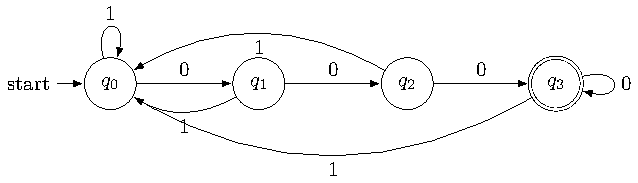
\includegraphics[width=0.7\textwidth]{automaton_1}
    \caption{DFA示例}
    \label{fig:DFA1}
\end{figure}

\newpage
图\ref{fig:DFA1}中的自动机的转移函数如表\ref{tab:DFA1}

\begin{table}[!htbp]
    \caption{图{\ref{fig:DFA1}}状态转移函数}
    \label{tab:DFA1}
    \centering
    \small% fontsize
    \setlength{\tabcolsep}{4pt}% column separation
    \renewcommand{\arraystretch}{1.2}%row space 
    \begin{tabular}{l p{3em}<{\centering} p{3em}<{\centering} p{3em}<{\centering}}
        \toprule %\hline 
        \multirow{2}{*}{状态说明} & \multirow{2}{*}{状态} & \multicolumn{2}{c}{输入字符} \\
		\cline{3-4}      &    &$0$ & $1$  \\
        \midrule%\hline
        开始状态(start)          & $q_0$ & $q_1$  & $q_0$    \\
                                & $q_1$ & $q_2$  & $q_0$    \\
                                & $q_2$ & $q_3$  & $q_0$    \\
        结束状态(final)         & $q_3$ & $q_3$  & $q_0$    \\
        \bottomrule%\hline  
    \end{tabular}
\end{table}

实例化$DFA$类如代码\ref{lst:DFASample}:

% \lstset{style=mystyle}
% \begin{lstlisting}[language=C++,label={lst:DFASample},caption={实例化DFA示例}]
% #include"DFA.h"
% #include<iostream>
% int main()
% {
%     DFA_components dfa_com1;

%     // StateSet S  开始状态集
%     dfa_com1.S.set_domain(10);
%     dfa_com1.S.add(0);

%     // StateSet F  结束状态集
%     dfa_com1.F.set_domain(10);
%     dfa_com1.F.add(3);

%     // StatePool Q 
%     int i = 10;
%     while (i--)
%     {
%         dfa_com1.Q.allocate();
%     }

%     // DTransRel T transition             
%     dfa_com1.T.set_domain(10);
%     dfa_com1.T.add_transition(0, '0', 1);
%     dfa_com1.T.add_transition(1, '0', 2);
%     dfa_com1.T.add_transition(2, '0', 3);
%     dfa_com1.T.add_transition(3, '0', 3);
%     dfa_com1.T.add_transition(0, '1', 0);
%     dfa_com1.T.add_transition(1, '1', 0);
%     dfa_com1.T.add_transition(2, '1', 0);
%     dfa_com1.T.add_transition(3, '1', 0);

%     DFA dfa1(dfa_com1);
%     dfa1.usefulf();

%     std::cout<<dfa1<<std::endl;
	
%     return 0;
% }
% \end{lstlisting}

代码 \ref{lst:DFASample} 将在控制台输出如下信息:
\lstset{style=mystyle}
\begin{lstlisting}[language=C++,label={lst:DFASampleLog},caption={图\ref{fig:DFA1}中自动机在 FIRE engine 中的表现形式}]
DFA
Q = [0,4)
S = { 0 }
F = { 3 }
Transitions =
0->{ '0'->1  '1'->0 }
1->{ '0'->2  '1'->0 }
2->{ '0'->3  '1'->0 }
3->{ '0'->3  '1'->0 }

current = -1
\end{lstlisting}

下文中将以表\ref{tab:DFA1}的形式来描述一个自动机,以代码\ref{lst:DFASampleLog}的形式来表示自动机在 FIRE engine 中的展现形式。实例化一个 DFA 时以 “实例化 DFA” 代指,不用代码表示。 
%!TEX root = ../Demo.tex
\chapter{测试内容}\label{cha:realwork}

本章内容为测试结果、测试过程中发现的问题、以及如何修复(部分)这些问题。

% \begin{remark}
%     因为$DFA$的最小化建立在状态等价性的基础之上,所以本文并未专门针对等价性进行测试。    
% \end{remark}
%%%%%%%%%%%%%%%%%%%%%%%%%%%%%%%%%%%%%%%%%%%%%%%%%%%%%%%%%%%%%%%%%%%%%%%%%%%%%%%%%%%%%%%%%%%%%%%%%%%%%%%%%%%%%%%%%%%%%%%%%%%%%%%%%%%%%%%%%%%%%%%%%
\section{如何测试}









%%%%%%%%%%%%%%%%%%%%%%%%%%%%%%%%%%%%%%%%%%%%%%%%%%%%%%%%%%%%%%%%%%%%%%%%%%%%%%%%%%%%%%%%%%%%%%%%%%%%%%%%%%%%%%%%%%%%%%%%%%%%%%%%%%%%%%%%%%%%%%%%%
\section{无限循环}\label{sec:ohloop}

实例化一个如表 \ref{tab:DFA4} 的 DFA 的对象之后,调用函数 DFA::min\_Watson()。(表 \ref{tab:DFA4} 对应的状态转移图为图 \ref{fig:DFA4_0},含有陷阱状态 $q_5$ \footnote{进入此状态之后无法通过任何转移离开,如图 \ref{fig:DFA4_0} 中的状态 {$q_5$}。} )

\begin{table}[!htbp]
    \caption{接受{$\mathcal{L}=0^*10^*$}的自动机{\cite{book1}}}
    \label{tab:DFA4}
    \centering
    \small% fontsize
    \setlength{\tabcolsep}{4pt}% column separation
    \renewcommand{\arraystretch}{1.2}%row space 
    %\begin{tabular}{lcrr} 
        \begin{tabular}{l p{3em}<{\centering} p{3em}<{\centering} p{3em}<{\centering}}
        \toprule %\hline 
        \multirow{2}{*}{状态说明} & \multirow{2}{*}{状态} & \multicolumn{2}{c}{输入字符} \\
		\cline{3-4}      &    &$0$ & $1$  \\
        \midrule%\hline
        开始状态(start)  & $q_0$ & $q_1$   & $q_2$   \\
                        & $q_1$ & $q_0$   & $q_3$   \\
        结束状态(final) & $q_2$ & $q_4$   & $q_5$   \\
        结束状态(final) & $q_3$ & $q_4$   & $q_5$   \\
        结束状态(final) & $q_4$ & $q_4$   & $q_5$   \\
        陷阱状态(sink) & $q_5$ & $q_5$   & $q_5$   \\
        \bottomrule%\hline 
    \end{tabular}
\end{table}

% {\bfseries 运行结果:} 函数进入无限循环
\subsection{运行结果}
函数进入无限循环。

% {\bfseries 错误原因:}
\subsection{错误原因} 

单步调试发现进入无限循环的位置为min-bww.cpp(124行),为代码 \ref{lst:minbww} 中的“H.equivalize(p, q);”。
\lstset{style=mystyle}
\begin{lstlisting}[language=C++,label={lst:minbww},caption={min-bww.cpp}]
if (are_eq(p, q, S, H, Z))
{
    // p and q are equivalent.
    H.equivalize(p, q);
}
\end{lstlisting}
单步进入该函数,可以看到代码 \ref{lst:StateEqRel} (StateEqRel.cpp(42行))
\lstset{style=mystyle}
\begin{lstlisting}[language=C++,label={lst:StateEqRel},caption={StateEqRel.cpp}]
for (oldq->iter_start(i); !oldq->iter_end(i); oldq->iter_end(i))
{
    map(i) = newp;
}
\end{lstlisting}
for循环的一般格式如代码 \ref{lst:for}
\lstset{style=mystyle}
\begin{lstlisting}[language=C++,label={lst:for},caption={for 循环的一般格式}]
for (初始化循环变量; 循环条件; 迭代)
{
    循环体
}
\end{lstlisting}
在代码 \ref{lst:StateEqRel} 中循环变量为“i”,循环条件为“!oldq->iter\_end(i);”,迭代为“oldq->iter\_end(i)”。查看“iter\_end()”函数实现如代码 \ref{lst:itend}
\lstset{style=mystyle}
\begin{lstlisting}[language=C++,label={lst:itend},caption={函数 iter\_end() 的实现}]
// StateSet.h
// Is r the last State in an iteration sequence.
inline int StateSet::iter_end(State r) const
{
	return(BitVec::iter_end(r));
}

// BitVec.h
// Is r the last set bit in an iteration sequence.
// if (r== -1) retrun 1; else return 0
inline int BitVec::iter_end(int r) const
{
	return(r == -1);
}
\end{lstlisting}
可以看到函数“iter\_end()”并未对参数“i”进行更改。于是程序在此处进入无限循环。

% {\bfseries 解决方法} :
\subsection{解决方法}

将代码 \ref{lst:StateEqRel} 中的迭代 “oldq->iter\_end(i)” 更改为 “oldq->iter\_next(i)”,更改后如代码 \ref{lst:StateEqRel2} ,经过比对,更改后与原文 \cite{watson1994design} 相同。
\lstset{style=mystyle}
\begin{lstlisting}[language=C++,label={lst:StateEqRel2},caption={StateEqRel.cpp}]
for (oldq->iter_start(i); !oldq->iter_end(i); oldq->iter_next(i))
{
    map(i) = newp;
}
\end{lstlisting}

{\bfseries 更改后}:函数“DFA::min\_Watson();”不再陷入无限循环。


%%%%%%%%%%%%%%%%%%%%%%%%%%%%%%%%%%%%%%%%%%%%%%%%%%%%%%%%%%%%%%%%%%%%%%%%%%%%%%%%%%%%%%%%%%%%%%%%%%%%%%%%%%%%%%%%%%%%%%%%%%%%%%%%%%%%%%%%%%%%%%%%%
%%%%%%%%%%%%%%%%%%%%%%%%%%%%%%%%%%%%%%%%%%%%%%%%%%%%%%%%%%%%%%%%%%%%%%%%%%%%%%%%%%%%%%%%%%%%%%%%%%%%%%%%%%%%%%%%%%%%%%%%%%%%%%%%%%%%%%%%%%%%%%%%%
\section{函数 DFA::usefulf() 运行错误}\label{sec:usefulf}

“DFA::usefulf()” 函数为一个重要函数。用于去除有限自动机中的非 “final-reachable” 状态,在执行最小化算法前执行该函数,可以去除有限自动机中的非“final-reachable”状态,进而减少程序运行时间。其定义如代码 \ref{lst:usefulf}
\lstset{style=mystyle}
\begin{lstlisting}[language=C++,label={lst:usefulf},caption={DFA::usefulf()}]
// Remove any States that cannot reach a final State.
// (This is a last step in minimization, since some of the min. algorithms may yield a DFA with a sink state.)
// Implement Remark 2.39  removing states that are not final - reachable.
DFA& usefulf();
\end{lstlisting}
以图 \ref{fig:DFA4_0} 为例,状态$q_5$ 即为非 “final-reachable” 状态(下称陷阱状态)。移除状态 $q_5$ 之后如图 \ref{fig:DFA4_1} 。图 \ref{fig:DFA4_1} 转移函数如表 \ref{tab:DFA4_1}。

\begin{table}[!htbp]
    \caption{接受{$\mathcal{L}=0^*10^*$}的自动机{\cite{book1}}}
    \label{tab:DFA4_1}
    \centering
    \small% fontsize
    \setlength{\tabcolsep}{4pt}% column separation
    \renewcommand{\arraystretch}{1.2}%row space 
    %\begin{tabular}{lcrr} 
        \begin{tabular}{l p{4em}<{\centering} p{3em}<{\centering} p{3em}<{\centering}}
        \toprule %\hline 
        \multirow{2}{*}{状态说明} & \multirow{2}{*}{状态} & \multicolumn{2}{c}{输入字符} \\
		\cline{3-4}      &    &$0$ & $1$  \\
        \midrule%\hline
        开始状态(start)  & $q_0$ & $q_1$   & $q_2$   \\
                        & $q_1$ & $q_0$   & $q_3$   \\
        结束状态(final) & $q_2$ & $q_4$   & -   \\
        结束状态(final) & $q_3$ & $q_4$   & -   \\
        结束状态(final) & $q_4$ & $q_4$   & -   \\
        \bottomrule%\hline 
    \end{tabular}
\end{table}

%%%%%%%%%%%%%%%%%%%%%%%%%%%%%%%%%%%%%%%%%%%%%%%%%%%%%%%%%%%%%%%%%%%%%%%%%%%%%%%%%%%%%%%%%%%%%%%%%%%%%%%%%%%%%%%%%%%%%%%%%%%%%%
% {\bfseries 运行结果}
\subsection{运行结果}

执行函数“DFA::usefulf()”后若状态 $q_5$ 被去除,则函数定义功能正常执行。但是在实际的执行过程中,程序提示如图 \ref{fig::usefulf_error} 错误 

\begin{figure}[!htbp]
    \centering
    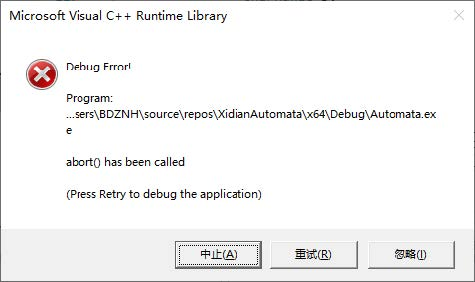
\includegraphics[width=0.60\textwidth]{DFA_usefulf_error}
    \caption{函数 DFA::usefulf() 错误提示}
    \label{fig::usefulf_error}
\end{figure}
控制台提示如图 \ref{fig::usefulf_console_log}
\begin{figure}[!htbp]
    \centering
    %trim option's parameter order: left bottom right top
    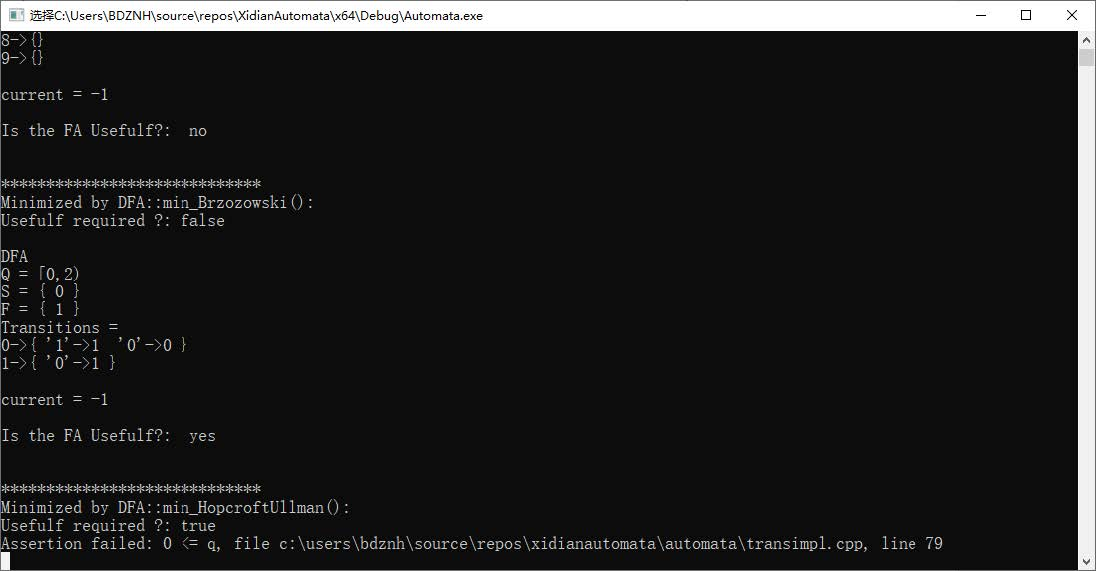
\includegraphics[trim = 0mm 0mm 0mm 63mm, clip,width=0.95\textwidth]{DFA_usefulf_console_log}
    \caption{函数 DFA::usefulf() 错误提示}
    \label{fig::usefulf_console_log}
\end{figure}

可以确定函数未完成其定义功能。

%%%%%%%%%%%%%%%%%%%%%%%%%%%%%%%%%%%%%%%%%%%%%%%%%%%%%%%%%%%%%%%%%%%%%%%%%%%%%%%%%%%%%%%%%%%%%%%%%%%%%%%%%%%%%%%%%%%%%%%%%%%%%%%%%%%%%%%%%%%%%%%%%%%%%%%%%%%%%%%%%%%%%%%%%%%%%
% {\bfseries 错误原因}
\subsection{错误原因}

查看 TransImple.cpp,79行,代码如下
\lstset{style=mystyle}
\begin{lstlisting}[language=C++,label={lst:TransImple},caption={ TransImple.cpp },firstnumber=75]
// Add a transition to the set.
TransImpl& TransImpl::add_transition(const CharRange a, const State q)
{
    assert(a.class_invariant());
    assert(0 <= q);
    ………
}
\end{lstlisting}

在 79 行处打断点,单步调试至此处,可以看到 State 变量 q 的值为“-842150451”,对应的十六进制值为“0xFFFFFFFF”\footnote{调试时使用 64 位编译器产生的二进制文件,在 64 位系统下运行。},为常见的未初始化错误。此时表达式 “0 <= q” 不成立,返回值为 “false” , 程序在此处中止。

查看函数 DFA::usefulf() 的实现,如代码 \ref{lst:DFA_usefulf_1} 。
\lstset{style=mystyle}
\begin{lstlisting}[language=C++,label={lst:DFA_usefulf_1},caption={ DFA.cpp },firstnumber=84]
StateTo<State> newnames;
newnames.set_domain(Q.size());

// All components will be constructed into a special structure :
DFA_components ret;
State st;
for (st = 0; st < Q.size(); st++)
{
    // If this is a Usefulf State, carry it over by giving it a name
    // in the new DFA.
    if (freachable.contains(st))
    {
        newnames.map(st) = ret.Q.allocate();
    }
}
\end{lstlisting}
在代码 \ref{lst:DFA_usefulf_1} 中将 “ final-reachable ” 状态保存到 StateTo<State> 变量 newnames 中,通过 “ ret.Q.allocate()” 为状态命名新的状态名,作为新的自动机的状态名。DFA\_components 变量 ret 用于构建新的自动机,再看函数内构造新的自动机的主要实现部分,如代码 \ref{lst:DFA_usefulf_2}
\lstset{style=mystyle}
\begin{lstlisting}[language=C++,label={lst:DFA_usefulf_2},caption={ DFA.cpp },firstnumber=130]
for (it = 0; !a.iter_end(it); it++)
{
    b = a.iterator(it);
    ret.T.add_transition(stprime, b, newnames.lookup(T.transition_on_range(st, b)));
}
\end{lstlisting}

根据代码 \ref{lst:TransImple} ,可以知道程序中止的地方为代码 \ref{lst:DFA_usefulf_2},133 行。其中 State 变量为当前需要进行操作的状态,CharRange 变量 b 为当前状态转移输入字符。查看 T.
transition\_on\_range(st, b)) 的实现,如代码 \ref{lst:transition_on_range}
\lstset{style=mystyle}
\begin{lstlisting}[language=C++,label={lst:transition_on_range},caption={ DTransRel.cpp },firstnumber=108]
// Compute the image of r, and CharRange it under *this.
inline State DTransRel::transition_on_range(const State r, const CharRange a) const
{
    assert(class_invariant());
    assert(0 <= r && r < domain());
    return(lookup(r).range_transition(a));
}
\end{lstlisting}
由代码 \ref{lst:transition_on_range} 可知,T.transition\_on\_range(st, b)) 将返回原自动机中,状态 st 经过输入字符 b 转移之后的目标状态。

查看 newnames.lookup() 的实现,如代码 \ref{lst:newnames-lookup}
\lstset{style=mystyle}
\begin{lstlisting}[language=C++,label={lst:newnames-lookup},caption={ StateTo.h },firstnumber=177]
// The actual mapping function
// First, a const lookup operator.
template<class T>
inline const T& StateTo<T>::lookup(const State r) const
{
    assert(class_invariant());
    // First check that it's in bounds
    assert(0 <= r && r < domain());
    return(data[r]);
}
\end{lstlisting}
在本例中,模板类 StateTo<T> 的模板参数 “T” 为 State。则 newnames.lookup(T.transition\_on\_range(st, b)) 为原自动机中 状态 st 经过字符 b 转移后的目标状态在新自动机中的状态。然后通过 ret.T.add\_transition() 保存新的转移关系。对所有的状态进行以上操作之后,通过变量 ret 构造新的自动机。 

经过单步调试发现,表\ref{tab:DFA4} 中,状态 $q_2$ 经过字符 “1” 将转移到状态 $q_5$,而在代码 \ref{lst:DFA_usefulf_1} 中,状态 $q_5$ 不满足 “if (freachable.contains(st))”,所以状态 $q_5$ 未被新的自动机保存,进而在代码 \ref{lst:DFA_usefulf_2} 中,当 st 为状态 $q_2$ 且 b 为字符 “1” 时,“newnames.lookup(T.transition\_on\_range(st, b))” 将返回未经初始化的值“-842150451”,于是在代码 \ref{lst:TransImple} 中,State 变量 q 的值为“-842150451”,导致程序在此处中止。

%%%%%%%%%%%%%%%%%%%%%%%%%%%%%%%%%%%%%%%%%%%%%%%%%%%%%%%%%%%%%%%%%%%%%%%%%%%%%%%%%%%%%%%%%%%%%%%%%%%%%%%%%%%%%%%%%%%%%%%%
\subsection{解决方法}

如代码 \ref{lst:State_H} 所示,文件 State.h 中将无效状态设置为 “Invalid”。在代码 \ref{lst:DFA_usefulf_1}增加处理不满足条件 “freachable.contains(st)” 的状态的内容,将原自动机中的非“final-reachable”状态标记为 “Invalid”,更改后为代码 \ref{lst:DFA_usefulf_1_edit}
\lstset{style=mystyle}
\begin{lstlisting}[language=C++,label={lst:DFA_usefulf_1_edit},caption={ 更改后的 DFA.cpp },firstnumber=91]
for (st = 0; st < Q.size(); st++)
{
    // If this is a Usefulf State, carry it over by giving it a name
    // in the new DFA.
    if (freachable.contains(st))
    {
        newnames.map(st) = ret.Q.allocate();
    }
    else                            // 新增
    {                               // 新增
        newnames.map(st) = Invalid; // 新增
    }                               // 新增
}
\end{lstlisting}

在代码 \ref{lst:DFA_usefulf_2} 中,在添加新的转移关系之前判断当前状态和目标状态是否都是有效状态,若都为有效状态,则添加新的转移关系。更改后为代码 \ref{lst:DFA_usefulf_2_edit}
\lstset{style=mystyle}
\begin{lstlisting}[language=C++,label={lst:DFA_usefulf_2_edit},caption={ 更改后的 DFA.cpp },firstnumber=133]
    State stdest;                                           // 新增
    stdest = newnames.lookup(T.transition_on_range(st, b)); // 新增

    if (stprime != Invalid &&  stdest != Invalid)           // 新增
    {                                                       // 新增
        ret.T.add_transition(stprime, b, stdest));          // 修改
    }                                                       // 新增
\end{lstlisting}

更改后函数 DFA::usefulf() 成功移除图 \ref{fig:DFA4_0} 中的陷阱状态 $q_5$ ,将图 \ref{fig:DFA4_0} 转换成图 \ref{fig:DFA4_1}。
更改后函数 DFA::usefulf() 成功移除图 \ref{fig:usefulf2-1} 中的陷阱状态 $q_1$ ,将图 \ref{fig:usefulf2-1} 转换成图 \ref{fig:usefulf2-2} 。



%%%%%%%%%%%%%%%%%%%%%%%%%%%%%%%%%%%%%%%%%%%%%%%%%%%%%%%%%%%%%%%%%%%%%%%%%%%%%%%%%%%%%%%%%%%%%%%%%%%%%%%%%%%%%%%%%%%%%%%%%%%%%%%%%%%%%%%%%%%%%%%%%%%%%%%%%%
%%%%%%%%%%%%%%%%%%%%%%%%%%%%%%%%%%%%%%%%%%%%%%%%%%%%%%%%%%%%%%%%%%%%%%%%%%%%%%%%%%%%%%%%%%%%%%%%%%%%%%%%%%%%%%%%%%%%%%%%%%%%%%%%%%%%%%%%%%%%%%%%%%%%%%%%%%
\section{函数 DFA::min\_Hopcroft() 运行错误}\label{sec:hopcroft}

% Hopcroft 算法描述如下\cite{watson1993taxonomyb} \\
% {\small \setlength{\parskip}{1em}
% \rule{\textwidth}{1pt}
% \mbox{ } $P:=[Q]_{E_0}$; \\
% \mbox{ } $L:= ( \mbox{\textbf{if }} ( |F| \leq |Q \setminus F | ) \mbox{\textbf{then }} \{F\} \mbox{\textbf{else }} \{ Q \setminus F \} \mbox{\textbf{fi }} ) \times V $; \\
% \mbox{ } $ \{ \mbox{恒有: } [Q]_E \sqsubseteq P \sqsubseteq [Q]_{E_0} \land L \subseteq (P \times V) $ \\
% \mbox{   } $ \land (\forall Q_0,Q_1,a:Q_0 \in Q \land (Q_1,a) \in L : \neg Splittable (Q_0,Q_1,a)) \Rightarrow (P=[Q]_E) \} $ \\
% \mbox{ } $ \mbox{\textbf{do }} L \not= \emptyset \longrightarrow $ \\ 
% \mbox{   } $ \mbox{\textbf{let }} Q_1,a:(Q_1,a) \in L $; \\
% \mbox{   } $ P_{old} := P $; \\
% \mbox{   } $ L := L \setminus \{ (Q_1,a) \} $; \\
% \mbox{   } $ \{  \mbox{恒有: } [Q]_E \sqsubseteq P \sqsubseteq P_{old} \} $ \\
% \mbox{   } $ \mbox{\textbf{for }} Q_0 : Q_0 \in P_{old} \land Splittable (Q_0,Q_1,a) \mbox{\textbf{ do }} $ \\
% \mbox{     } $ Q'_0 := \{ p:p \in Q_0 \land T(p,a) \in Q_1 \} $; \\
% \mbox{     } $ P:= P \setminus \{ Q_0 \} \cup \{ Q_0 \setminus Q'_0,b \} $;\\
% \mbox{     } $ \mbox{\textbf{for }} b:b \in V \mbox{\textbf{ do }} $ \\
% \mbox{       } $ \mbox{\textbf{if }} (Q_0,b) \in L \rightarrow L := L \setminus \{ (Q_0,b) \} \cup \{ (Q'_0,b),(Q_0, \setminus Q'_0,b ) \} $;\\ 
% \mbox{       } $ \talloblong (Q_0,b) \notin L \rightarrow $ \\
% \mbox{         } $ L := L \cup (\mbox{\bfseries if} ( |Q'_0| \leq |Q_0 \setminus Q'_0| ) \mbox{\bfseries then} \{ (Q'_0 , b) \} \mbox{\bfseries else} \{ ( Q'_0 \setminus Q'_0,b ) \} \mbox{\bfseries fi} ) $ \\
% \mbox{       } $ \mbox{\textbf{fi}} $ \\
% \mbox{     } $ \mbox{\textbf{rof}} $ \\
% \mbox{   } $ \mbox{\textbf{rof}} $ \\
% \mbox{   } $ \{ (\forall Q_0,Q_0 \in P : \neg Splittable(Q_0,Q_1,a)) \} $ \\
% \mbox{ } $ \mbox{\textbf{od }} \{ P = [Q]_E \} $ \\
% \rule{\textwidth}{1pt} }

实例化如表 \ref{tab:DFA411-1} 所示的自动机。(含有开始不可达状态\footnote{从开始状态不可以到达的状态,如图 \ref{fig:DFA11-0} 中状态 $q_9$ 。}(start-unreachable))

\begin{table}[!htbp]
    \caption{图\ref{fig:DFA11-0}的转移函数}
    \label{tab:DFA411-1}
    \centering
    \small% fontsize
    \setlength{\tabcolsep}{4pt}% column separation
    \renewcommand{\arraystretch}{1.2}%row space 
    %\begin{tabular}{lcrr} 
        \begin{tabular}{l p{4em}<{\centering} p{3em}<{\centering} p{3em}<{\centering}}
        \toprule %\hline 
        \multirow{2}{*}{状态说明} & \multirow{2}{*}{状态} & \multicolumn{2}{c}{输入字符} \\
		\cline{3-4}      &    &$0$ & $1$  \\
        \midrule%\hline
        开始状态(start)  & $q_0$ & $q_1$   & $q_2$   \\
                        & $q_1$ & $q_5$   & $q_2$   \\
                        & $q_2$ & $q_3$   & $q_6$   \\
                        & $q_3$ & $q_2$   & $q_4$   \\
        结束状态(final) & $q_4$ & $q_8$   & $q_1$   \\
                        & $q_5$ & $q_1$   & $q_6$   \\
                        & $q_6$ & $q_7$   & $q_2$   \\
                        & $q_7$ & $q_6$   & $q_8$   \\
        结束状态(final) & $q_8$ & $q_5$   & $q_4$   \\
        开始不可达状态    & $q_9$ & $q_7$   & $q_5$   \\
        \bottomrule%\hline 
    \end{tabular}
\end{table}

函数 DFA::min\_Hopcroft() 是 Hopcroft 算法在 FIRE engine 中的实现,Hopcroft 算法在文中\cite{watson1993taxonomyb}描述如下:
\begin{figure}[!htbp]
    \centering
        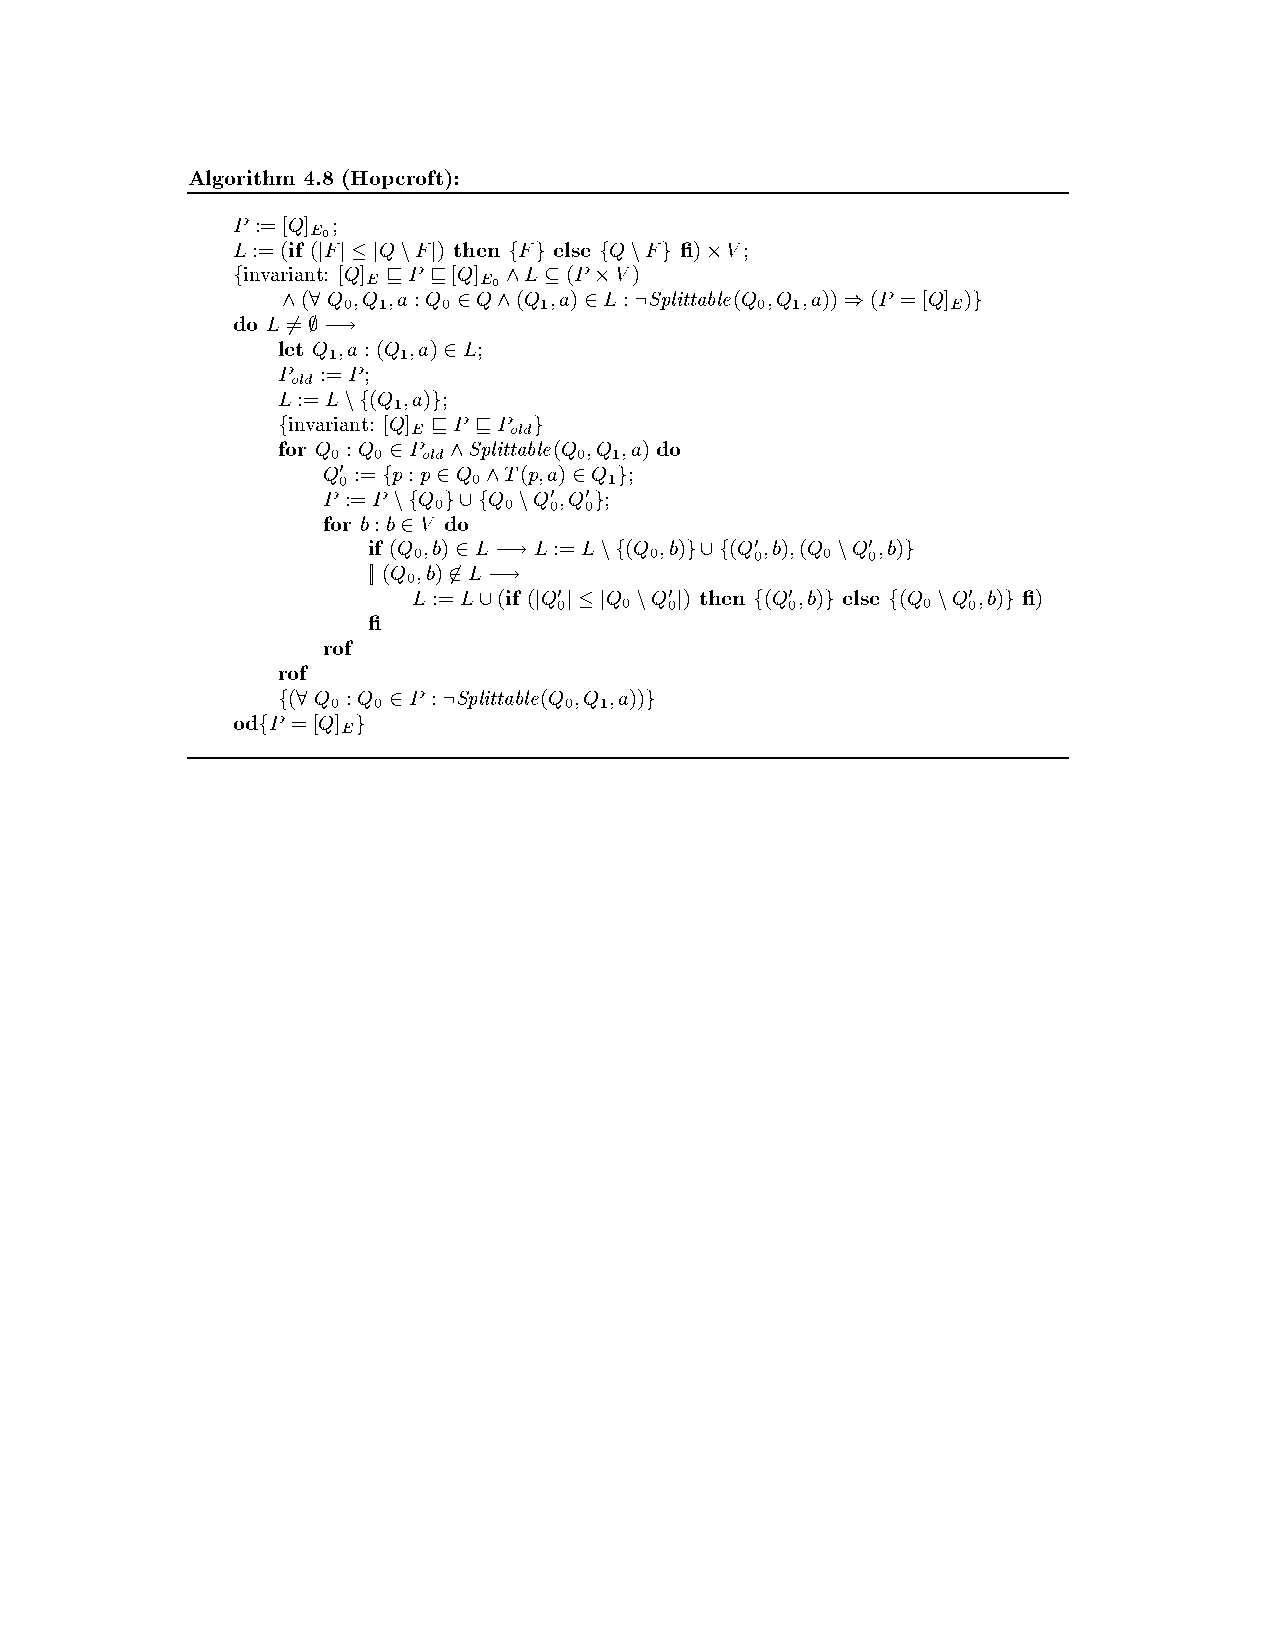
\includegraphics[width=0.99\textwidth]{hopcroft}
\end{figure}

\subsection{运行结果}\label{sec:hopcroft-error}
执行函数 DFA::min\_Hopcroft(),程序在文件CRSet.h,第 146 行的 “assert(!iter\_end(it))” 处触发 assert 中止,如代码 \ref{lst:iterend} 所示。调用函数“CRSet::iterator()”的地方为文件min-hop.cpp,第103行,“State r(split(p, q, C.iterator(L[q]), P));”的“C.iterator(L[q])”处。
\lstset{style=mystyle}
\begin{lstlisting}[language=C++,label={lst:iterend},caption={ CRSet.h },firstnumber=142]
// Fetch the it'th CharRange in *this.
inline const CharRange& CRSet::iterator(const int it) const
{
    assert(class_invariant());
    assert(!iter_end(it));
    return(data[it]);
}

// Is there even in it'th CharRange?
inline int CRSet::iter_end(const int it) const
{
    assert(class_invariant());
    assert(0 <= it);
    return(it >= in_use);
}
\end{lstlisting}

\subsection{错误原因}

以表 \ref{tab:DFA411-1} 中实例化的自动机为例,CRSet 变量 C = \{ 0, 1\},在程序中止处打断点,调试至此处可看到 int 变量 it 为 “2”,因 C 中只有两个值 “1、2”,所以传入参数为 “2” 时,超出可以 C 的范围,于是在语句 “assert(!iter\_end(it));” 处导致程序中止。

算法迭代过程如附录表 \ref{tab:hopcroft} 所示。

在第 11 次迭代中,DFA::split() 函数将等价类\{0,1,5\} 分割为等价类 \{\{0\},\{1,5\}\},此时$p=0,q=0,r=1$,满足条件$|Q'_0| \leq | Q_0 \setminus Q'_0 |$,执行 L[r] = L[p] =1,L[p] = C.size() = 2。在第 12 次迭代中,由于第 11 次迭代中 $p=q$ ,所以 L[q] 的值将被更改为 “2”,于是在 C.iterator(L[q]) 处传入一个超过 C 的范围的值,程序触发 assert 中止。

\subsection{解决方法}

函数 DFA::min\_Hopcroft() 的主要实现部分如代码 \ref{lst:hopcroft-iter}。
\lstset{style=mystyle}
\begin{lstlisting}[language=C++,label={lst:hopcroft-iter},caption={ min-hop.cpp },firstnumber=100]
    for (repr.iter_start(p); !repr.iter_end(p); repr.iter_next(p))
    {
        //分割等价类
        ……
    }
\end{lstlisting}

在分割等价类之前,判断 L[q] 是否等于 “C.size()”,若是,则减去 “1”,更改后为代码 \ref{lst:hopcroft-iter-edit}

\lstset{style=mystyle}
\begin{lstlisting}[language=C++,label={lst:hopcroft-iter-edit},caption={ min-hop.cpp },firstnumber=100]
    for (repr.iter_start(p); !repr.iter_end(p); repr.iter_next(p))
    {
        if(L[q] == C.size()) // 新增
        {                    // 新增
            L[q]--;          // 新增
        }                    // 新增
        //分割等价类
        ……
    }
\end{lstlisting}

更改后函数 DFA::min\_Hopcroft() 运行不再中止。

%%%%%%%%%%%%%%%%%%%%%%%%%%%%%%%%%%%%%%%%%%%%%%%%%%%%%%%%%%%%%%%%%%%%%%%%%%%%%%%%%%%%%%%%%%%%%%%%%%%%%%%%%%%%%%%%%%%%%%%%%%%%%%%%
%%%%%%%%%%%%%%%%%%%%%%%%%%%%%%%%%%%%%%%%%%%%%%%%%%%%%%%%%%%%%%%%%%%%%%%%%%%%%%%%%%%%%%%%%%%%%%%%%%%%%%%%%%%%%%%%%%%%%%%%%%%%%%%%
\section{测试结果汇总}

经过 \ref{sec:ohloop} 节、\ref{sec:usefulf} 节和 \ref{sec:hopcroft} 节的修改,FIRE engine 中的最小化算法及最小化算法用到的帮助函数都可以成功运行。本节内容为测试正确的结果和一些未能解决的问题的汇总。

\subsection{不改变已经是最小的 DFA 接受的语言}

接受一个 $\mathcal{L}$ 的最小的 DFA 是唯一的,最小的且接受相同 $\mathcal{L}$ 的 DFA 仅仅在状态命名上有差别\cite{book1}。因此最小化算法有性质 \ref{sec:keepMin} 。

\begin{property}\label{sec:keepMin}
    由定义 \ref{def:min} 可知,对于 DFA $M$,$\mathcal{L}(Min(M))= \mathcal{L}(M)$,同样的,最小化算法不能使最小的 DFA 接受的 $\mathcal{L}$ 发生改变。
\end{property}

\begin{remark}
    DFA 中的 开始不可达(start-unreachable)状态和陷阱状态(final-unreachable)状态不影响 DFA 接受的 $\mathcal{L}$。
\end{remark}



\begin{table}[!htbp]
    \caption{一组最小的 DFA}
    \label{tab:KeepMinData}
    \centering
    \small% fontsize
    \setlength{\tabcolsep}{4pt}% column separation
    \renewcommand{\arraystretch}{1.2}%row space 
    \begin{tabular}{c p{4em}<{\centering} p{4em}<{\centering} l}  %l p{3em}<{\centering} p{3em}<{\centering} p{3em}<{\centering}
        \toprule %\hline 
                序号  &  数据 & 属性 & 备注 \\
        \midrule%\hline
        1 &  图 \ref{fig:usefulf2-1} & 最小的 & 含有陷阱状态 \\
        2 &  图 \ref{fig:usefulf2-2} & 最小的 & 不含陷阱状态 \\
        \midrule
        3 & 图 \ref{fig:DFA11-0} & 最小的 & 含有开始不可达状态 \\
        4 & 图 \ref{fig:DFA11-1} & 最小的 & 不含开始不可达状态 \\
       \midrule
        5 & 图 \ref{fig:keepMin-1-unreachable} & 最小的 & 含有开始不可达状态 \\
        6 & 图 \ref{fig:keepMin-1-nonTheState} & 最小的 & 不含开始不可达状态 \\
       \midrule
        7 & 图 \ref{fig:keepMin-2-unreachable} & 最小的 & 含有开始不可达状态 \\
        8 & 图 \ref{fig:keepMin-2-nonTheState} & 最小的 & 不含开始不可达状态 \\
        \bottomrule%\hline  
    \end{tabular}
\end{table}


对于性质 \ref{sec:keepMin} ,以表 \ref{tab:KeepMinData} 中的一组最小的 DFA 为数据,测试结果表 \ref{tab:KeepMinResult} 所示。




\begin{table}[!htbp]
    \caption{ 最小化算法对性质 \ref{sec:keepMin} 的测试结果 }
    \label{tab:KeepMinResult}
    \centering
    \small% fontsize
    \setlength{\tabcolsep}{4pt}% column separation
    \renewcommand{\arraystretch}{1.2}%row space 
    \begin{tabular}{l|p{2em}<{\centering} p{2em}<{\centering} p{2em}<{\centering} p{2em}<{\centering} p{2em}<{\centering} p{2em}<{\centering} p{2em}<{\centering} p{2em}<{\centering}}  %l p{3em}<{\centering} p{3em}<{\centering} p{3em}<{\centering}
        \toprule %\hline 
        算法 & 1 & 2 & 3 & 4 &  5 &  6  & 7 & 8  \\
        \midrule
        DFA::min\_Brzozowski()        & $\surd$ & $\surd$ & $\times$  & $\times$  & $\checkmark$ & $\surd$ & $\checkmark$ & $\surd$ \\
        DFA::min\_Hopcroft()(修改前) & $\surd$ & $\surd$ & 中止    & $\surd$     & $\surd$ & $\surd$ & $\surd$ & $\surd$ \\
        DFA::min\_Hopcroft()(修改后) & $\surd$ & $\surd$ & $\surd$ & $\surd$     & $\surd$ & $\surd$ & $\surd$ & $\surd$ \\
        DFA::min\_HopcroftUllman()    & $\surd$ & $\surd$ & $\surd$ & $\surd$     & $\surd$ & $\surd$ & $\surd$ & $\surd$ \\
        DFA::min\_dragon()            & $\surd$ & $\surd$ & $\surd$ & $\surd$     & $\surd$ & $\surd$ & $\surd$ & $\surd$ \\
        DFA::min\_Watson()            & $\surd$ & $\surd$ & $\surd$ & $\surd$     & $\surd$ & $\surd$ & $\surd$ & $\surd$ \\
        \bottomrule%\hline  
    \end{tabular}
\end{table}

对表 \ref{tab:KeepMinResult} 中的测试结果有两个算法需要额外关注—— “DFA::min\_Brzozowski()” 和 “DFA::min\_Hopcroft()”。

结果总结对比如下:
\begin{itemize}
    \item 对于 DFA 中的陷阱状态,可以调用函数 “DFA::usefulf()” 函数去除。表 \ref{tab:KeepMinResult} 中在执行最小化函数之前,除了算法 “DFA::min\_Brzozowski”, 都执行了函数 “DFA::usefulf()”;
    \item 除了算法 “DFA::min\_Brzozowski()” 外,其他最小化算法均不能去除 DFA 中的开始不可达状态(start-unreachable)。数据为第 5 个和第 7 个,以 $\checkmark$ 标示,而不是 $\surd$;
    \item 对于算法 “DFA::min\_Hopcroft()” 的 assert 中止,在发生 assert 中止的第 3 个数据中,含有开始不可达状态,作为对照组且含有开始不可达状态的第 5 个和第 7 个数据确没有发生 assert 中止,所以本文认为此算法的中止的问题不是 DFA 中开始不可达状态导致;
    \item 对于第 3 个和第 4 个数据,算法 “DFA::min\_Brzozowski()” 改变了 DFA ,输入的 DFA 仅有 10/9 个状态,算法 “DFA::min\_Brzozowski()” 输出了含有数百个状态的自动机。
\end{itemize}



\subsection{最小化功能测试}

本节内容为最小化算法对定义功能的测试,以表 \ref{tab:MinData} 中的数据对五个最小化算法进行测试,结果如表 \ref{tab:MinResult} 所示。

\begin{table}[!htbp]
    \caption{一组 DFA}
    \label{tab:MinData}
    \centering
    \small% fontsize
    \setlength{\tabcolsep}{4pt}% column separation
    \renewcommand{\arraystretch}{1.2}%row space 
    \begin{tabular}{c p{4em}<{\centering} p{4em}<{\centering} c }  %l p{3em}<{\centering} p{3em}<{\centering} p{3em}<{\centering}
        \toprule %\hline 
                序号  &  数据 & 属性 & 预期结果  \\
        \midrule%\hline
        1 &  图 \ref{fig:DFA4_0} &            & 图 \ref{fig:DFA4_3}\\
        \midrule
        2 & 图 \ref{fig:DFAMin-3-0} &         & 图 \ref{fig:DFAMin-3-2}  \\
        3 & 图 \ref{fig:DFAMin-3-1} & 最小的  & 图 \ref{fig:DFAMin-3-1}  \\
        \midrule
        4 & 图 \ref{fig:DFAMin-5-0} &         & 图 \ref{fig:DFAMin-5-2}  \\
        5 & 图 \ref{fig:DFAMin-5-1} & 最小的  & 图 \ref{fig:DFAMin-5-1}  \\
        \midrule
        6 & 图 \ref{fig:DFAMin-4-0} &        & 图 \ref{fig:DFAMin-4-2}  \\
        7 & 图 \ref{fig:DFAMin-4-1} & 最小的  & 图 \ref{fig:DFAMin-4-1}  \\
        \bottomrule%\hline  
    \end{tabular}
\end{table}

\begin{table}[!htbp]
    \caption{ 最小化算法的定义功能的测试结果 }
    \label{tab:MinResult}
    \centering
    \small% fontsize
    \setlength{\tabcolsep}{4pt}% column separation 
    \renewcommand{\arraystretch}{1.2}%row space 
    \begin{tabular}{l| p{2em}<{\centering} p{2em}<{\centering} p{2em}<{\centering} p{2em}<{\centering} p{2em}<{\centering} p{2em}<{\centering} p{2em}<{\centering} }  %l p{3em}<{\centering} p{3em}<{\centering} p{3em}<{\centering}
        \toprule %\hline 
        算法 & 1 & 2 & 3 & 4 &  5 & 6 & 7 \\
        \midrule
        DFA::min\_Brzozowski()        & $\surd$ & $\surd$ & $\surd$   & $\surd$ & $\surd$ & $\surd$     & $\surd$       \\
        DFA::min\_Hopcroft()(修改前) & $\surd$ & $\surd$ & $\times$  & $\surd$ & $\surd$ & 中止        & $\surd$       \\
        DFA::min\_Hopcroft()(修改后) & $\surd$ & $\surd$ & $\times$  & $\surd$ & $\surd$ & $\surd$     & $\surd$       \\
        DFA::min\_HopcroftUllman()    & $\surd$ & $\surd$ & $\surd$   & $\surd$ & $\surd$ & $\surd$     & $\surd$       \\
        DFA::min\_dragon()            & $\surd$ & $\surd$ & $\surd$   & $\surd$ & $\surd$ & $\surd$     & $\surd$       \\
        DFA::min\_Watson()            & $\surd$ & $\surd$ & $\surd$   & $\surd$ & $\surd$ & $\surd$     & $\surd$       \\
        \bottomrule%\hline  
    \end{tabular}
\end{table}

对于第 3 个数据,算法 “DFA::min\_Hopcroft()” 无论是否经过第 \ref{sec:hopcroft} 节的修改,均输出代码 \ref{lst:hoperrorResult} 。
\lstset{style=mystyle}
\begin{lstlisting}[language=C++,label={lst:hoperrorResult},caption={ 第 3 个数据在算法 “DFA::min\_Hopcroft()” 中的输出 }]
DFA
Q = [0,2)
S = { 0 }
F = { 1 }
Transitions =
0->{ ['a','b']->1 }
1->{ 'a'->1 }

current = -1
\end{lstlisting}

第 3 个数据的转移函数如表 \ref{tab:sample_3_origin} 所示 ,代码 \ref{lst:hoperrorResult} 的转移函数如表 \ref{tab:sample_3_result} 所示 

% \begin{table}[!htbp]
%     \caption{接受{$\mathcal{L}=0^*10^*$}的自动机{\cite{book1}}}
%     \label{tab:hopcroftErrorResult}
%     \centering
%     \small% fontsize
%     \setlength{\tabcolsep}{4pt}% column separation
%     \renewcommand{\arraystretch}{1.2}%row space 
%     %\begin{tabular}{lcrr} 
%         \begin{tabular}{l p{3em}<{\centering} p{3em}<{\centering} p{3em}<{\centering}}
%         \toprule %\hline 
%         \multirow{2}{*}{状态说明} & \multirow{2}{*}{状态} & \multicolumn{2}{c}{输入字符} \\
% 		\cline{3-4}      &    &$0$ & $1$  \\
%         \midrule%\hline
%         开始状态(start)  & $q_0$ & $q_1$   & $q_2$   \\
%                         & $q_1$ & $q_0$   & $q_3$   \\
%         结束状态(accept) & $q_2$ & $q_4$   & $q_5$   \\
%         结束状态(accept) & $q_3$ & $q_4$   & $q_5$   \\
%         结束状态(accept) & $q_4$ & $q_4$   & $q_5$   \\
%         陷阱状态(sink) & $q_5$ & $q_5$   & $q_5$   \\
%         \bottomrule%\hline 
%     \end{tabular}
% \end{table}

\begin{table}[!htbp]
    \caption{第 3 个数据在算法 “DFA::min\_Hopcroft()” 中的输入输出对比 }
    \label{tab:sample_3}
    \centering
    \small% fontsize
    \setlength{\tabcolsep}{4pt}% column separation
    \renewcommand{\arraystretch}{1.2}%row space 
    \begin{subtable}[t]{0.45\textwidth}
        \centering
        \caption{输入}
        \label{tab:sample_3_origin}
        \begin{tabular}{l p{2em}<{\centering} c c}
            \toprule%\hline
            \multirow{2}{*}{状态说明} & \multirow{2}{*}{状态} & \multicolumn{2}{c}{输入字符} \\
            \cline{3-4}      &    &$a$ & $b$  \\
            %\cline{2-9}% partial hline from column i to column j
            \midrule%\hline
            开始状态(start)  & $q_0$ & $q_1$   & $q_2$   \\
            结束状态(final) & $q_1$ & $q_2$   &     -   \\
            结束状态(final) & $q_2$ & -       & $q_1$   \\
            \bottomrule%\hline
        \end{tabular}
    \end{subtable}
    ~% add desired spacing
    \begin{subtable}[t]{0.45\textwidth}
        \centering
        \caption{输出}
        \label{tab:sample_3_result}
        \begin{tabular}{l p{2em}<{\centering} c c }
            \toprule%\hline
            \multirow{2}{*}{状态说明} & \multirow{2}{*}{状态} & \multicolumn{2}{c}{输入字符} \\
            \cline{3-4}      &    & $a$ & $b$  \\
            %\cline{2-9}% partial hline from column i to column j
            \midrule%\hline
            开始状态(start)  & $q_0$ & $q_1$   & $q_1$   \\
            结束状态(final) & $q_1$ & $q_1$   & -   \\
            ---------------& --& - & - \\
            \bottomrule%\hline
        \end{tabular}
    \end{subtable}
\end{table}

图 \ref{fig:DFAMin-3-1} 原本是一个最小的 DFA,由表 \ref{tab:sample_3} 可知,函数算法 “DFA::min\_Hopcroft()” 已经改变了图 \ref{fig:DFAMin-3-1} 的状态数,由 “3” 变到 “2”, 如图 \ref{fig:DFAMinHoop-3} 所示,已经不满足性质 \ref{sec:keepMin}。由此可以认为 FIRE engine 中算法 “DFA::min\_Hopcroft()” 未完成其定义功能。

\begin{figure}[!htbp]
    \centering
    \begin{subfigure}[b]{0.4\textwidth}
        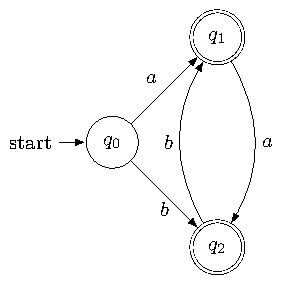
\includegraphics[width=\textwidth]{Min/DFAMinTest-3-1}
        \caption{输入}
        \label{fig:DFAMin-3-1-inside}
    \end{subfigure}
    ~
    \begin{subfigure}[b]{0.4\textwidth}
        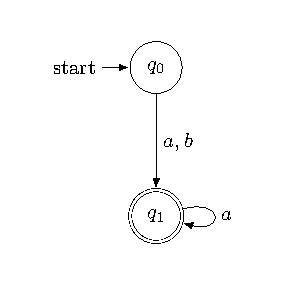
\includegraphics[width=\textwidth]{Min/DFAMinTest-3-3}
        \caption{输出}
        \label{fig:DFAMin-3-3-inside}
    \end{subfigure}
    \caption{DFA::min\_Hopcroft 对第 3 个数据输入输出对比}
    \label{fig:DFAMinHoop-3}
  \end{figure}

对于算法 “DFA::min\_Hopcroft()” 和算法 “DFA::min\_Brzozowski” 的扩展测试见附录。


%!TEX root = ../Demo.tex
\chapter{引言}
自动机理论是许多科学的重要理论基础,从硬件电路的简化,到各式各样的编译器构造,到处都有着自动机理论的应用,从自动机理论的诞生开始,自动机的最小化就一直是一个重要的关注点,因为自动机的状态数约少,意味着它使用的资源也会越少,这一点对资源敏感的自动机应用很重要。已经有很多人为此做了大量的工作。1954 年,Huffman 提出了经典的用于确定性有限自动机的最小化算法\cite{HUFFMAN1954161},随后更高效的最小化算法由 Hopcroft 和 Moore 提出。确定性有限自动机(Deterministic Finite Automata,DFA)的最小化是自动机理论的一个重要组成部分,研究确定性有限自动机的最小化对自动机理论的健全和发展有重要意义。

\section{FIRE engine}
FIRE engine \cite{watson1994design}是 Stellenbosch 大学的 Bruce William Watson 教授使用C++语言实现一个用于有限自动机和正则表达式的类库。本文中也把“有限自动机C++工具箱”称作 “FIRE engine” 。有限自动机C++工具箱(下称 FIRE engine)实现了论文 \cite{watson1993taxonomya,watson1993taxonomyb} 中提及的大部分算法,其中也包括了 Hopcroft、Ullman 等人提出的著名的确定性有限自动机最小化算法,验证这些算法的正确性和有效性对研究其他最小化算法很有帮助。

\section{国内外研究现状}

自动机理论的发展已经有很长时间,有限状态自动机、确定性有限状态自动机及相关的理论出现的时间都比较早。国外已经有文章 \cite{watson1993taxonomyb} 对一些著名的确定性有限自动机最小化算法,如 Hopcroft、Brzozowski、Ullman 等提出的最小化算法和这些算法之间的演化关系做出了详尽的阐述。

据称 Hopcroft 的算法有着最优的时间复杂度, 此算法时间复杂度为 $\mathcal{O}$($n$ log $n$)\cite{Hopc71}。严格来说,Hopcroft 的算法的时间复杂度不仅仅与自动机的大小 $n$ \footnote{ $n$ 为自动机的状态数,也称自动机的大小。}有关,还与自动机的输入的字母表的大小 $k$ 有关,其时间复杂度应为$\mathcal{O}$($kn$ log $n$)。Timo Knuutila 指出,在自动机的输入的字母表的大小不固定时,Hopcroft 的原始算法的时间复杂度将不再是$\mathcal{O}$($kn$ log $n$)\cite{KNUUTILA2001333}。

以状态的等价为基础,通过分层逼近、逐点近似等方法来计算等价关系,并在此基础上衍生处其他最小化算法。文中提及的算法中,Brzozowski 的最小化算法不依赖于其他任何最小化算法,也不依赖于确定状态的等价,而其他著名的算法的基础都是状态等价,是在已有的算法上的改进\cite{watson1993taxonomyb}。

国内对最小化算法的研究则针对一些更加详细的分类。比如在胡芙提出的超最小化算法,用来把确信性树自动机转换为确定性有限自动机,然后用等价状态合并和等价类分割,最后得到差异有限的确定性树自动机\cite{hfTreeFA}。还有张锋的基于 Myhill-Nerode 原理推导出来的针对直觉模糊有限自动机和完备格上的直觉模糊有限自动机的最小化算法\cite{zf14Min}。对于自动机技术的实际应用,孙丹丹在海量的 Web 信息中抽取用户需要的信息上应用了模糊树自动机技术,并且提出模糊树自动机的构造算法和最小化算法\cite{sdd14}。 

\section{本文的工作}

第\ref{cha:preliminaries}章内容为确定性有限自动机最小化需要的预备知识,用来帮助理解。第\ref{cha:construct-dfa} 章则介绍 FIRE engine 中 对类 DFA 的实现和实例化类 DFA 所必须的其他的类,给出实例化类 DFA 对象所需要的步骤。第\ref{cha:realwork}章则是在测试过程中遇到的问题和解决这些问题的步骤。

本文的主要使用 Visual Studio 2017 集成开发环境,对 FIRE engine 实现的最小化算法进行功能测试,验证 FIRE engine 的中的最小化算法的有效性。
%!TEX root = ../Demo.tex
\chapter{预备知识}\label{cha:preliminaries}

在进行本文的叙述之前,需要预先了解一些相关的知识和定义,以便于使用更加简洁的描述方式。

德国数学家在 1874 年提出集合论(set theory),经过长时间的发展和完善,集合论成为了数学的一个重要组成部分,并且已经渗透到许多领域。计算机科学出现并发展壮大的过程中,集合论也成为计算机理论的一个重要基础概念。

集合论的最基础的概念是集合,集合的一个非形式描述为:一定范围内确定的,并且彼此可以区分的对象汇集在一起形成的整体叫做集合(set)\cite{book1}。



%%%%%%%%%%%%%%%%%%%%%%%%%%%%%%%%%%%%%%%%%%%%%%%%%%%%%%%%%%%%%%%%%%%%%%%%%%%%%%%%%%%%%%%%%%%%%%%%%%%%%%%%%%%%%%%%%%%%%%%%%%%%%%%%%%%%%%%%%%%%%%%%%%%%%%%%%%%%%%%%%%%%%%%%%%%%%%%%%%%%%%%%%%%%%%%%%%%%%%%%
\section{基本定义}

\begin{definition}[幂集\cite{watson1993taxonomyb}] \label{pro:mathP}
    对于任意集合$A$,我们使用$\mathcal{P}(A)$代表$A$的所有子集。$\mathcal{P}(A)$也叫做$A$的幂集。有时也写作 $2^A$。
\end{definition}

\begin{example}[集合的幂集]
    设集合 $A=\{a,b\}$,那么 $ \mathcal{P}(A) = \{\emptyset,\{a\},\{b\},\{a,b\} \} $,$\mathcal{P}(A)$ 等价于 $2^A$。
\end{example}

\begin{definition}[函数集\cite{watson1993taxonomyb}]
    对于集合 $A$ 和 $B$ ,$A\to B$代表所有从$A$到$B$的函数的集合。
\end{definition}

\begin{definition}[笛卡尔积\cite{book1}]
    对于集合 $A$ 和 $B$,$A$ 和 B 的的笛卡尔积是一个集合。该集合满足
    \[
        A \times B = \{ (a,b) | a \in A \land b \in B \}    
    \]
\end{definition}

\begin{definition}[二元关系\cite{watson1993taxonomyb,book1}]
    对于集合 $A$ 和 $B$,$\mathcal{C} \subseteq A \times B$ 是 $A \to \mathcal{P}(B)$ 的二元关系。
\end{definition}

\begin{definition}[关系的合成\cite{watson1993taxonomyb,book1}]
    对于集合 $A$、$B$ 、 $C$,和关系 $\mathcal{R}_0 \subseteq A \times B$、$\mathcal{R}_1 \subseteq B \times C$,$\mathcal{R}_0$ 和 $\mathcal{R}_1$ 的合成定义为
    \[ 
        \mathcal{R}_0 \circ \mathcal{R}_1 = A \to C = \{ (a,c) | \exists (a,b) \in \mathcal{R}_0 \land (b,c) \in \mathcal{R}_2 \}
    \]
\end{definition}
% \begin{definition}[等价类]
%     something to write。
% \end{definition}

\begin{definition}[等价关系的等价类\cite{watson1993taxonomyb}]\label{def:equiv-class}
    对任何集合 $A$ 上的等价关系 $E$,我们使用 $[A]_E$代表等价类\footnote{等价关系和等价类稍后说明} 集合,即:
$$ [A]_E = \{ [a]_E :a \in A \} $$
集合 $[A]_E$ 也叫做 $A$ 的由 $E$ 引出的划分(partition)。
\end{definition}

\begin{definition}[等价类的指数\cite{watson1993taxonomyb}]
    对于集合$A$上的等价关系$E$,定义$\sharp E = | [A]_E |$。$\sharp E$ 也叫做$E$的“指数”。
\end{definition}


\begin{definition}[字母表\cite{watson1993taxonomyb}] \label{def:Alphabat}
    字母表是有限大小的非空集合。
\end{definition}

\begin{definition}[等价关系的细化]
    对于等价关系$E$和$E'$(在集合$A$上),当且仅当$E \subseteq E'$,$E$是$E'$的细化(refinement)。
\end{definition}













%%%%%%%%%%%%%%%%%%%%%%%%%%%%%%%%%%%%%%%%%%%%%%%%%%%%%%%%%%%%%%%%%%%%%%%%%%%%%%%%%%%%%%%%%%%%%%%%%%%%%%%%%%%%%%%%%%%%%%%%%%%%%%%%%%%%%%%%%%%%%%%%%%%%%%%%%%%%%%
\section{有限自动机}

本小节中定义有限自动机、其性质和用于有限自动机的变换。本节内容大部分直接引用自\cite{watson1993taxonomyb}。

\begin{remark}[状态转移图\cite{watson1993taxonomya}]
    一般来说,我们使用状态转移图来表示一个自动机,如图\ref{fig:state_graph}
\end{remark}

% 一般来说,我们使用状态转移图来表示一个自动机,如图\ref{fig:state_graph}

\begin{figure}[!htbp]
    \centering
    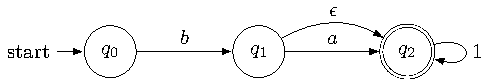
\includegraphics[width=0.7\textwidth]{state_graph}
    \caption{自动机状态转移图}
    \label{fig:state_graph}
\end{figure}

图\ref{fig:state_graph}中,自动机由$q_0$进入,接收字符“b”转移到状态$q_1$,状态$q_1$接收字符“a”转移到状态$q_2$,图中的两个同心圆圈住状态$q_2$表示结束状态( final state )或者接受状态( accepted state ),意味自动机处理字符串到达此状态时,自动机就接受当前处理的字符串,状态$q_2$上有一个指向自己的箭头,意为接收字符“1”之后,仍然指向自己。而状态$q_1$经过$\epsilon$转移到状态$q_2$,意为状态$q_1$可以不接收任何字符即可转移到状态$q_2$。%图\ref{fig:state_graph}中的自动机接受的字符串为$\mathcal{L}=ba(1)^*\cup b(1)^*$。

\begin{definition}[有限自动机 \cite{watson1993taxonomyb}]
    有限自动机(Finite Automata,FA)是一个6元组$(Q,V,T,E,S,F)$,其中
    \begin{itemize}
        \item $Q$ 是有限状态集;
        \item $V$ 是一个字母表;
        \item $ T \in \mathcal{P}(P\times V \times Q) $是一个转移关系;
        \item $ E \in \mathcal{P}(Q\times Q)$ 是一个$\epsilon$-转移关系(空转移,不需要接收字符即可转移);
        \item $ S \subseteq Q $是开始状态集;
        \item $ F \subseteq Q $是结束状态集;
    \end{itemize}
    字母表和函数$\mathcal{P}$的定义分别在“定义\ref{def:Alphabat}” 和 “定义 \ref{pro:mathP}”。
\end{definition}

\begin{example}
    我们可以用$M=(\{q_0,q_1,q_2\},\{b,a,1,\epsilon\},T,E,\{q_0\},\{q_2\})$来指代图\ref{fig:state_graph}中的自动机。其中,$T=\{(q_0 \times b \times q_1),(q_1\times a \times q_2),(q_2\times 1 \times q_2)\}$,$E=(q_1 \times q_2)$。
\end{example}

\begin{remark}
    为了在某些情况下方便的展示状态之间的关系,也把状态转移图写成表格\cite{book1},如图\ref{fig:state_graph}中的自动机,写成表 \ref{tab:sample}:
\begin{table}[!htbp]
    \caption{状态转移函数}
    \label{tab:sample}
    \centering
    \small% fontsize
    \setlength{\tabcolsep}{6pt}% column separation
    \renewcommand{\arraystretch}{1.2}%row space 
    % \begin{tabular}{l p{4em}<{\centering} p{2em}<{\centering} p{2em}<{\centering} p{2em}<{\centering} p{2em}<{\centering}} 
    \begin{tabular}{lccccc}
        \toprule%\hline 
        \multirow{2}{*}{状态说明} & \multirow{2}{*}{状态} & \multicolumn{4}{c}{输入字符} \\
		\cline{3-6}      &    & $a$ & $b$ & $1$ & ${\epsilon}$ \\
        %                        &        & \multicolumn{4}{c}{输入字符} \\
        %\cline{3-6}  {状态说明}  & {状态} &$a$ & $b$ & $1$ & $\epsilon$ \\
        \midrule%\hline
        开始状态(start)  & $q_0$ & -     & $q_1$  &      - &     -    \\
                        & $q_1$ & $q_2$ &    -   &    -   &    $q_2$ \\
        结束状态(final) & $q_2$ &   -   & -      & $q_2$  &    -     \\
        \bottomrule%\hline 
    \end{tabular}
\end{table}
\end{remark}


%\newpage
表格\ref{tab:sample}的状态之间的关系与$T=\{(q_0 \times b \times q_1),(q_1\times a \times q_2),(q_2\times 1 \times q_2)\}$,$E=(q_1 \times q_2)$一一对应,“\mbox{-}” 表示没有相应的转移关系。%%下文中将表格\ref{tab:sample}简称为转移函数。

\begin{remark}[转移关系的表示]
    为了更加简洁的描述转移关系,用 “$T=(q_0 \times b \times q_1)$” 来代表图 \ref{fig:state_graph} 中的 “状态 $q_0$ 接收字符 ‘b’ 转移到状态 $q_1$”。
\end{remark}

\begin{remark}
    本文在不同情况下使用不同的形式来表示转移关系,比如,对于转移关系 $T=(q_0 \times b \times q_1)$ ,也写成 $ q_1 = T(q_0 , b) $。对于图 \ref{fig:state_graph} 中状态 $q_0$ 和 $q_2$ 之间的转移关系,可以描述为 $T(q_0\times w \times q_2)$ 或者 $q_2=T(q_0 , w)$,其中,$w=ba$ 或 $w=b\epsilon$。
\end{remark}

\subsection{有限自动机的性质}

本小节定义有限自动机(Finite automata,下称 FA)的性质,为了使定义更加简洁,引进三个特殊的 FA: $M=(Q,V,T,E,S,F)$ , $M_0=(Q_0,V_0,T_0,E_0,S_0,F_0)$ , $ M_1=(Q_1,V_1,T_1,E_1,S_1,F_1) $。

\begin{definition}[FA 的大小]
    定义一个FA的大小为$|M|=|Q|$。
\end{definition}

\begin{definition}[FA 的同构$\cong$]\label{def:isom}
    我们把同构定义为FA的等价关系。当且仅当 $V_0=V_1$,并且存在双射$g\in Q_0 \longrightarrow Q_1$ ,使得
\begin{itemize}
    \item $T_1 = \{ (g(p,q),a,g(q)) : (p,a,q) \in T_0 \}$
    \item $E_1 = \{ (g(p,q),a,g(q)) : (p,q) \in E_0\}$
    \item $S_1 = \{ g(s):s\in S_0 \}$
    \item $F_1 = \{ g(f):f\in F_0 \}$
\end{itemize}
时$M_0$和$M_1$是同构的(写作$M_0 \cong M_1$)。
\end{definition}

\begin{definition}[转移关系 $T$ 的扩展]
    我们把$T \in V \longrightarrow \mathcal{P} (Q \times Q) $ 到 $ T^* \in V^* \longrightarrow \mathcal{P} (Q \times Q)  $的转换关系以如下方式扩展: 
    \[ 
        T^*(\epsilon) = E^* 
    \]
    且对于$(a\in V,w\in V^*)$ 有 
    \[ 
        T^*(aw) = E^* \circ T(a) \circ T^*(w)    
    \]
    操作符$\circ$在定义 2.5 中定义。
\end{definition}

\begin{definition}[左语言和右语言 \cite{watson1993taxonomyb}]
    状态($M$中)的左语言由函数$ \overleftarrow{\mathcal{L}} _M \in Q \longrightarrow \mathcal{P}(V^*)$ 给出,其中:
    \[ 
        \overleftarrow{\mathcal{L}}_M (q) = ( \cup s:s \in S : T^*(s,q) )  
    \] 
    状态($M$中)的右语言由函数$ \overrightarrow{\mathcal{L}} _M \in Q \longrightarrow \mathcal{P}(V^*)$给出,其中 
    \[ 
        \overrightarrow{\mathcal{L}}_M (q) = ( \cup f:f \in F : T^*(q,f) ) 
    \] 
    通常在没有歧义的时候移除下标$M$。
\end{definition}

\begin{definition}[ FA 的语言 \cite{watson1993taxonomyb}]
    有限自动机的语言由函数 $\mathcal{L}_{FA} \in FA \longrightarrow \mathcal{P}(V^*) $给出,该函数的定义为式 \ref{eq:languageoffa}: 
    \begin{equation}\label{eq:languageoffa}
        \mathcal{L}_{FA} (M) = (\cup s,f:s \in S \land f \in F : T^* (s,f))
    \end{equation}
\end{definition}

\begin{example}[FA 的语言]
    图 \ref{fig:state_graph} 中的 FA 接受的语言为 $ \mathcal{L}= \{ ba(1)^*\cup b(1)^* \}$。下文中使用符号 $\mathcal{L}$ 代替 FA 接受的 “语言”。
\end{example}

\begin{definition}[完全 FA ($Complete$)\cite{watson1993taxonomyb}]\label{def:complete}
    一个完全 FA 满足式 (\ref{eq:complete} ):
    \begin{equation} \label{eq:complete}
        Complete(M) \equiv ( \forall q,a:q\in Q \land a \in V : T(q,a) \not= \emptyset ) 
    \end{equation}
\end{definition}

\begin{definition}[$\epsilon$-$free$]
    当且仅当 $E=\emptyset$时,$M$ 是 $\epsilon$-$free$ 的。
\end{definition}

\begin{definition}[可达状态 \cite{watson1993taxonomya}]\label{def:rechable-state}
    可达状态分为 “开始可达状态” 和 “可达结束状态” ( $M$ 中),其中
    \begin{itemize}
        \item 开始可达状态:从开始状态可以到达的状态,写作 $SReachable(M)$;
        \item 可达结束状态: 能到达结束状态的状态,写作 $FReachable(M)$;
    \end{itemize}
    可达状态定义为:
    \[ Reachable(M) = SReachable(M) \cap FReachable(M) \]
\end{definition}

\begin{definition}[Start-useful 自动机\cite{watson1993taxonomyb}]
    一个 $Useful_s$ 自动机 定义如下: 
    \[ Useful_s (M) \equiv ( \forall q:q \in Q : \overleftarrow{\mathcal{L}} (q) \not= \emptyset ) \]
\end{definition}

\begin{definition}[Final-useful 自动机\cite{watson1993taxonomyb}]
    一个 $Useful_f$ 自动机 定义如下: 
    \[ Useful_f (M) \equiv ( \forall q:q \in Q : \overrightarrow{\mathcal{L}} (q) \not= \emptyset ) \]
\end{definition}

\begin{definition}[Useful 自动机\cite{watson1993taxonomyb}]
    $Useful$ 自动机是一个只有可达状态的 FA:
    \[ Useful (M) \equiv Useful_s (M) \land Useful_f (M) \]
\end{definition}

\begin{example}
    如图 \ref{fig:UsefulFA} 所示,其中
    \begin{itemize}
        \item 图 \ref{fig:UsefulFA-2} 为一个 $Useful$ FA;
        \item 图 \ref{fig:UsefulFA-1} 中状态 $q_1$ 不是一个开始可达状态,也称开始不可达状态(start-unreachable);
        \item 图 \ref{fig:UsefulFA-1} 中状态 $q_2$ 不是一个可达结束状态,也称陷阱状态(final-unreachable)\cite{book1}。
    \end{itemize}
\end{example}

\begin{figure}[!htbp]
    \centering
    \begin{subfigure}[b]{0.45\textwidth}
        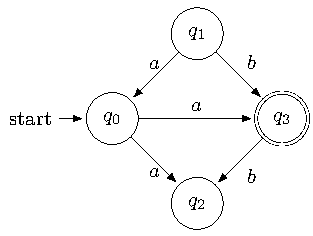
\includegraphics[width=\textwidth]{UsefulFA-1}
        \caption{}
        \label{fig:UsefulFA-1}
    \end{subfigure}
    ~
    \begin{subfigure}[b]{0.45\textwidth}
        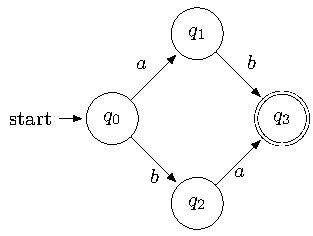
\includegraphics[width=\textwidth]{UsefulFA-2}
        \caption{}
        \label{fig:UsefulFA-2}
    \end{subfigure}
    \caption{}
    \label{fig:UsefulFA}
\end{figure}

\begin{definition}[确定的有限自动机 \cite{watson1993taxonomyb}]
    当且仅当 
    \begin{itemize}
        \item 无多重开始状态;
        \item 无$\epsilon$转移关系;
        \item 转移函数$T \in Q \times V \longrightarrow \mathcal{P} (Q) $ 不将 $Q \times V$ 映射至多个状态。
    \end{itemize}
    时有限自动机$M$是确定的,称 $M$ 为确定的有限自动机(Deterministic Finite Automata,下称 DFA)。
    公式形式表达为式 \ref{eq:DetFA} :
    \begin{equation}\label{eq:DetFA}
    Det(M) \equiv ( |S| \leq 1 \land \epsilon\mbox{-} free(E) \land ( \forall q,a:q \in Q \land a \in V : |T(q,a)| \leq 1 )) 
    \end{equation}
    且有$ DFA \subseteq FA$。
\end{definition}


\begin{definition}[DFA 的最小化\cite{watson1993taxonomyb}]\label{def:min}
    满足以下条件时,$M\in DFA$是最小的:
    { \small \[  Min(M) \equiv (\forall M' : M' \in DFA \land Complete(M') \land \mathcal{L}(M) = \mathcal{L}_{FA}(M') : |M| \leq |M'| ) \] }
函数 $Min$ 仅定义在 DFA 上。一个最小的但是仍然完全的 DFA 的定义如下:
{\small \[  Min_{\mathcal{C}}(M) \equiv ( \forall M':M' \in DFA \land Complete(M') \land \mathcal{L}_{FA}(M) = \mathcal{L}_{FA}(M'): |M| \leq |M'| ) \] }
$Min_{\mathcal{C}}$ 仅定义在完全 DFA 上。
\end{definition}

\subsection{有限自动机的变换}

\begin{transformation}[FA 的反转(reversal)\cite{watson1993taxonomyb}]\label{trans:reverse}
        $FA$反转由上标函数$ R \in FA \to FA $ 给出,它的定义如下:
        \[ (Q,V,T,S,F)^R = (Q,V,T^R,E^R,F,S) \]
    函数 $R$ 满足
    \[ (\forall M : M \in FA : ( \mathcal{L}_{FA} (M) )^R = \mathcal{L}_{FA}(M^R)) \]
\end{transformation}

\begin{transformation}[移除开始状态不可达状态\cite{watson1993taxonomyb}]\label{trans:usefuls}
    变换$useful_s \in FA \longrightarrow FA$移除开始状态不可达状态:
    \begin{table}[!htbp]
        \centering
        %\small% fontsize
        \setlength{\tabcolsep}{1pt}% column separation
        \renewcommand{\arraystretch}{1.3}%row space 
        \begin{tabular}{lcll} 
            $useful_s(Q,V,T,E,S,F)$ & = & {\bfseries let} & $U = SReachable(Q,V,T,E,S,F)$ \\
                                    &   & {\bfseries in}  &                               \\
                                    &   &                 & $(U,V,T \cap (U\times V \times U), E \cap (U \times U), S \cap U, F \cap U )$  \\
                                    &   & {\bfseries end} &                               \\
        \end{tabular}
    \end{table}
% \\除了性质 $ \mathcal{L}_{FA}(subset(M))= \mathcal{L}_{FA}(M) $(对所有的$M \in FA$)之外,
 \\ 函数 $ useful_s $ 满足
\[  (\forall M : M \in FA : Useful_s ( useful_s(M) ) \land \mathcal{L}_{FA} (useful_s(M)) = \mathcal{L}_{FA}(M)) \]
\end{transformation}

% \begin{transformation}[子集构造\cite{watson1993taxonomyb}]
%     函数$subset$把一个$\epsilon$-$free$ FA 转换为一个 DFA (在子句 \textbf{let} $T'\in \mathcal{P}(Q) \times V \longrightarrow \mathcal{P}(\mathcal{P} (Q) )$ 中): 
%     \begin{table}[!htbp]
%         \centering
%         %\small% fontsize
%         \setlength{\tabcolsep}{4pt}% column separation
%         \renewcommand{\arraystretch}{1.4}%row space 
%         \begin{tabular}{lcll} 
%             $subset(Q,V,T,\emptyset,S,F)$ & = & {\bfseries let} & $T'(U,a) = \{ (q:q\in U : T(q,a) ) \} $ \\
%                                           &   &                 & $F'= \{ U : U \in \mathcal{P}(Q) \land U \cap F \not= \emptyset \} $ \\
%                                           &   & {\bfseries in}  &                                         \\
%                                           &   &                 & $ ( \mathcal{P}(Q),V,T',\emptyset,\{ S \},F' ) $  \\
%                                           &   & {\bfseries end} &                               \\
%         \end{tabular}
%     \end{table}
%     \\除了性质 $ \mathcal{L}_{FA}(subset(M))= \mathcal{L}_{FA}(M) $(对所有的$M \in FA$)之外,函数 $subset$ 还满足
%     \[ (\forall M : M \in FA \land \epsilon \mbox{-} free(M) : Det(subset(M)) \land Complete(subset(M))) \]
%     有时候也把它说成“幂集”构造。
% \end{transformation}

\begin{definition}[优化的子集构造\cite{watson1993taxonomyb}]
    函数$subsetopt$把一个$\epsilon$-$free$ $FA$ 转换为一个 DFA。%此函数是$subset$的一个优化版本:
    \begin{table}[!htbp]
        \centering
        %\small% fontsize
        \setlength{\tabcolsep}{2pt}% column separation
        \renewcommand{\arraystretch}{1.3}%row space 
        \begin{tabular}{lcll} 
            $subsetopt(Q,V,T,\emptyset,S,F)$ & = & {\bfseries let} & $ T'(U,a) = \{ (q:q\in U : T(q,a) ) \} $ \\
                                          &   &                 & $ Q' = \mathcal{P} (Q) \setminus \{ \emptyset \} $ \\
                                          &   &                 & $ F'= \{ U : U \in \mathcal{P}(Q) \land U \cap F \not= \emptyset \} $ \\
                                          &   & {\bfseries in}  &                                         \\
                                          &   &                 & $ ( Q',V,T' \cap (Q' \times V \times Q'),\emptyset,\{ S \},F' ) $  \\
                                          &   & {\bfseries end} &                               \\
        \end{tabular}
    \end{table}
    \\除了性质$\mathcal{L}_{FA} (subsetopt(M)) = \mathcal{{L}} (M) $(对所有的$M\in FA$)之外,函数$subsetopt$还满足
    $$ ( \forall M : M \in FA \land \epsilon \mbox{-}free(M) : Det(subset(M)) )  $$
\end{definition}

\section{等价性和最小化}

令 $M=\{Q,V,T,\emptyset,S,F \}$ 为一个完全 DFA,并且 $M$ 中所有状态都是可达状态。

\begin{definition}[状态的等价\cite{watson1993taxonomyb}]
    当$M$ 中的状态 $ p,q $ 满足式 (\ref{eq:equivalence}) 时,称状态 $p,q$ 等价。
    \begin{equation} \label{eq:equivalence}
        (p,q) \in E \equiv ( \overrightarrow{\mathcal{L}}(p) = \overrightarrow{\mathcal{L}}(q) )
    \end{equation}
    其中,$E$ 为等价关系(Equivalence)。
\end{definition}

\begin{definition}[状态的等价\cite{book1}]
    给出状态等价的另一种描述。对给定的 $DFA$ $M=(Q,V,T,\emptyset,S,F)$,如果 $\exists w \in V^*$ ,使得$Q$ 中的两个状态 $p$ 和 $q$,若$T(q,w)\in F$ 和 $T(p,w)\in F$ 有且仅有一个成立,那么称 $p$ 和 $q$ 是可区分的,否则称 $p$ 和 $q$ 等价,写作 $p \equiv q$。
\end{definition}

\begin{remark}
    关系 $D$ (Distinguishable) 是可区分的状态,$E$ 和 $D$ 满足 $D=\lnot E$。
\end{remark}

\begin{remark}[操作符 $\setminus$]
    $M$ 中,若 $p \in (Q \setminus F)$ , 那么 $ p \notin F$。
\end{remark}

\begin{remark}
    $\forall p,q: p \in (Q \setminus F) \land q \in F$,有 $ p \not\equiv q $。
\end{remark}

\subsection{最小化}

最小化是对于一个给定的 DFA $M$,找到一个与 $M$ 接受同样的 $\mathcal{L}$ 的且状态数最少的 DFA $M_1$ ($|M_1|\leq |M|$)的过程, 最小化算法用来计算 DFA 中的关系 $D$ 和关系 $E$,只需计算其中一个即可得到 $M_1$ \cite{watson1993taxonomyb}(本文仅针对 DFA 应用最小化算法)。

给出一种用于 DFA 的最小化算法\cite{book1,zf14Min,yingjie2009describing},描述如算法 \ref{ali:classic-al} 所示:

\begin{algorithm}
    \caption{经典算法(也称标记法\cite{zf14Min})}\label{ali:classic-al}
    \begin{algorithmic}[1]
        \Require DFA $M$
        \Ensure 与 $M$ 同构的最小的 DFA
        \Statex
        \State $ \forall (p,q) \in (Q \setminus F) \times F $,标记状态对 $(p,q)$ 
        \Repeat
            \ForAll {未被标记的状态对$(p,q)$ }
                \ForAll {$\forall x \in V$}
                    \If {状态对$ (T(p,x),T(q,x)) $ 被标记了}
                        \State 标记状态对$(p,q)$
                    \EndIf
                \EndFor
            \EndFor
        \Until{没有新的状态对被标记}
    \end{algorithmic}
\end{algorithm}

\begin{theorem}
    算法 \ref{ali:classic-al} 的时间复杂度为 $\mathcal{O}(n^2)$ \cite{yingjie2009describing}。
\end{theorem}

\begin{theorem}
    算法 \ref{ali:classic-al} 移除不可达状态后的 DFA 为最小的 DFA \cite{book1}。
\end{theorem}

% \begin{enumerate}[1.]
%     \item $ \forall (p,q) \in (Q \setminus F) \times F $,标记可区分状态表中的表项 $(p,q)$ 
%     \item $ \forall (p,q) \in (Q \setminus F) \times \in (Q \setminus F) \cup F \times F \land p \not =  q $ ,进行以下步骤:
%     \item 如果 $\exists a \in V $,若可区分状态表项 $(T(p,a),T(q,a))$ 已经被标记,那么继续标记可区分状态表 $(p,q)$;
%     \item 递归重复步骤 2 ,步骤 3 ;
%     \item 否则 $\forall a \in V $,如果 $T(p,a) \not= T(q,a) $ 且 $(p,a)$ 与  $(T(p,a),T(q,a))$ 不是同一个状态对,那么将 $(p,q)$ 放在  $(T(p,a),T(q,a))$ 的关联表上。
% \end{enumerate}

% \begin{remark}
%     本文把等价状态的集合叫做等价类。
% \end{remark}
% 其中
% \begin{itemize}
%     \item 可区分状态表,用来标记状态对是否可以被区分。如果相应的表项可以被区分,则使用 $\checkmark$ 标示。
%     \item 状态关联表。
% \end{itemize}

\begin{example}
    使用算法 \ref{ali:classic-al} 对图 \ref{fig:DFAMin-3-0-minexample} 中的 DFA 进行最小化。
\end{example}

\begin{figure}[!htbp]
    \centering
    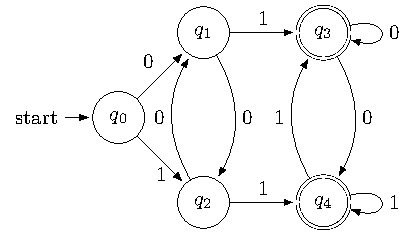
\includegraphics[width=0.6\textwidth]{Min/markAlexample}
    \caption{一个接受 $\mathcal{L}=\{ 0(0)^*1(0|1)^* \cup 1(0)^*1(0|1)^*  \}$ 的 DFA }
    \label{fig:DFAMin-3-0-minexample}
\end{figure}


\begin{enumerate}[(1)]
    \item 首先标记状态对$(q_0,q_3)$,$(q_0,q_4)$,$(q_1,q_3)$,$(q_1,q_4)$,$(q_2,q_3)$,$(q_2,q_4)$。剩下需要计算的状态对为$(q_0,q_1)$,$(q_0,q_2)$,$(q_1,q_2)$,$(q_3,q_4)$;
    \item 对于状态对$(q_0,q_1)$,$T(q_0,0)=q_1$,$T(q_1,0)=q_2$,此时状态对$(q_1,q_2)$未被标记,无操作;再看$T(q_0,1)=q_2$,$T(q_1,1)=q_3$,此时$(q_0,q_3)$已经被标记,那么标记状态对$(q_0,q_1)$;
    \item 对于状态对$(q_0,q_2)$,$T(q_0,0)=q_1$,$T(q_2,0)=q_1$,不做处理,再看$T(q_0,1)=q_2$,$T(q_2,1)=q_4$,此时状态对$(q_0,q_4)$已经被标记,那么标记$(q_0,q_2)$;
    \item 对于状态对$(q_1,q_2)$,$T(q_1,0)=q_2$,$T(q_2,0)=q_1$,不做处理,再看$T(q_1,1)=q_3$,$T(q_2,1)=q_4$,此时状态对$(q_3,q_4)$未被标记,无操作;
    \item 对于状态对$(q_3,q_4)$,$T(q_3,0)=q_3$,$T(q_4,0)=q_3$,不做处理,再看$T(q_3,1)=q_4$,$T(q_4,1)=q_4$,不做处理;
    \item 第一次迭代结束,此时还有状态对$(q_1,q_2)$和$(q_3,q_4)$未被标记。
    \item 对于状态对$(q_1,q_2)$,根据第(4)步,算法无操作;
    \item 对于状态对$(q_3,q_4)$,根据第(5)步,算法无操作;
    \item 本次迭代未标记任何状态对,算法结束,此时还有状态对$(q_1,q_2)$和$(q_3,q_4)$未被标记。
\end{enumerate}

算法结束后还有状态对$(q_1,q_2)$和$(q_3,q_4)$未被标记,也就是说$q_1 \equiv q_2$,$q_3 \equiv q_4$。此时的 DFA 为图 \ref{fig:DFAMin-3-0-minexample-rel}。

\begin{figure}[!htbp]
    \centering
    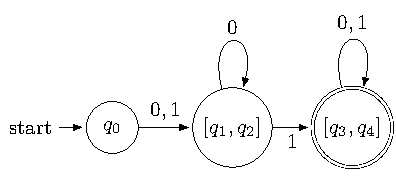
\includegraphics[width=0.5\textwidth]{Min/markAlexample-rel}
    \caption{与图 \ref{fig:DFAMin-3-0-minexample} 同构的最小的 DFA }
    \label{fig:DFAMin-3-0-minexample-rel}
\end{figure}


\chapter{等价关系和最小化}

% {\heiti 这是一段黑体字}

% {\rmfamily rmfamily}

% {\ttfamily ttfamily 1234567890 ABCDEFGQWE}

% {\fangsong 普通仿宋字体}

% {\fangsong\bfseries 加粗仿宋字体}

% Xidian University

% \begin{table}[!htbp]
%     \caption{状态转移函数}
%     \label{tab:sample2}
%     \centering
%     \small% fontsize
%     \setlength{\tabcolsep}{4pt}% column separation
%     \renewcommand{\arraystretch}{1.2}%row space 
%     \begin{tabular}{l|c|c|c|c|c} 
%         \hline
%         参数 & 条件 & Min & Typ & Max & 单位 \\
%         \hline
%         \multicolumn{6}{l}{湿度} \\
%         \hline
%         \multirow{2}{*}{分辨率} & \multirow{2}{*}{ } & 1 & 1 & 1 & RH \\

%         \cline{3-6}            &                    &   & 16 &  &  Bit \\
%         \hline
%     \end{tabular}
% \end{table}

% \begin{algorithm}
%     \caption{Euclid’s algorithm}\label{euclid}
%     \begin{algorithmic}[1]
%         \Procedure{Euclid}{$a,b$}\Comment{The g.c.d. of a and b}
%         \State $r\gets a\bmod b$
%         \While{$r\not=0$}\Comment{We have the answer if r is 0}
%         \State $a\gets b$
%         \State $b\gets r$
%         \State $r\gets a\bmod b$
%         \EndWhile\label{euclidendwhile}
%         \State \textbf{return} $b$\Comment{The gcd is b}
%         \EndProcedure
%         \do $L \not= \emptyset \longrightarrow $ 
        
%     \end{algorithmic}
% \end{algorithm}

% \mbox{ } $P:=[Q]_{E_0}$; \\
% \mbox{ } $L:= ( \mbox{\textbf{if }} ( |F| \leq |Q \setminus F | ) \mbox{\textbf{then }} \{F\} \mbox{\textbf{else }} \{ Q \setminus F \} \mbox{\textbf{fi }} ) \times V $; \\
% \mbox{ } $ \{ \mbox{恒有: } [Q]_E \sqsubseteq P \sqsubseteq [Q]_{E_0} \land L \subseteq (P \times V) $ \\
% \mbox{   } $ \land (\forall Q_0,Q_1,a:Q_0 \in Q \land (Q_1,a) \in L : \neg Splittable (Q_0,Q_1,a)) \Rightarrow (P=[Q]_E) \} $ \\
% \mbox{ } $ \mbox{\textbf{do }} L \not= \emptyset \longrightarrow $ \\ 
% \mbox{   } $ \mbox{\textbf{let }} Q_1,a:(Q_1,a) \in L $; \\
% \mbox{   } $ P_{old} := P $; \\
% \mbox{   } $ L := L \setminus \{ (Q_1,a) \} $; \\
% \mbox{   } $ \{  \mbox{恒有: } [Q]_E \sqsubseteq P \sqsubseteq P_{old} \} $ \\
% \mbox{   } $ \mbox{\textbf{for }} Q_0 : Q_0 \in P_{old} \land Splittable (Q_0,Q_1,a) \mbox{\textbf{ do }} $ \\
% \mbox{     } $ Q'_0 := \{ p:p \in Q_0 \land T(p,a) \in Q_1 \} $; \\
% \mbox{     } $ P:= P \setminus \{ Q_0 \} \cup \{ Q_0 \setminus Q'_0,b \} $;\\
% \mbox{     } $ \mbox{\textbf{for }} b:b \in V \mbox{\textbf{ do }} $ \\
% \mbox{       } $ \mbox{\textbf{if }} (Q_0,b) \in L \rightarrow L := L \setminus \{ (Q_0,b) \} \cup \{ (Q'_0,b),(Q_0, \setminus Q'_0,b ) \} $;\\ 
% \mbox{       } $ \talloblong (Q_0,b) \notin L \rightarrow $ \\
% \mbox{         } $ L := L \cup (\mbox{\bfseries if} ( |Q'_0| \leq |Q_0 \setminus Q'_0| ) \mbox{\bfseries then} \{ (Q'_0 , b) \} \mbox{\bfseries else} \{ ( Q'_0 \setminus Q'_0,b ) \} \mbox{\bfseries fi} ) $ \\
% \mbox{       } $ \mbox{\textbf{fi}} $ \\
% \mbox{     } $ \mbox{\textbf{rof}} $ \\
% \mbox{   } $ \mbox{\textbf{rof}} $ \\
% \mbox{   } $ \{ (\forall Q_0,Q_0 \in P : \neg Splittable(Q_0,Q_1,a)) \} $ \\
% \mbox{ } $ \mbox{\textbf{od }} \{ P = [Q]_E \} $ \\

% \begin{algorithm}
%     \caption{Euclid’s algorithm}\label{euclid}
%     \begin{program}
%         $P:=[Q]_{E_0}$;
%         $L:= ( \mbox{\textbf{if }} ( |F| \leq |Q \setminus F | ) \mbox{\textbf{then }} \{F\} \mbox{\textbf{else }} \{ Q \setminus F \} \mbox{\textbf{fi }} ) \times V $;
%     \end{program}
% \end{algorithm}

\section{等价关系}

等价关系是进行 DFA 最小化的基础,本节定义状态的等价及一些应用。
\chapter{实例化类DFA对象}

\section{DFA类}
在本文中,我们仅仅对 DFA 应用最小化算法,FIRE engine 中的DFA类为应用最小化算法的类。
FIRE engine 提供了多种方式构造一个 DFA,类 DFA 的部分实现如表 \ref{tab:Class-DFA} 
% \lstset{style=mystyle}
% \begin{lstlisting}[language=C++,label={lst:consDFA},caption={class DFA}]
% class DFA : virtual public FAabs
% {
% public:
%     // Default copy constructor, destructor, operator= are okay.
%     inline DFA();

%     // A special constructor used for subset construction etc.
%     inline DFA(const DFA_components& r);
%     ……
%     StatePool Q;
%     // S must be a singleton set, or empty. |S| <= 1
%     StateSet S;
%     StateSet F;  // final states
%     DTransRel T;
% }
% ……
% inline DFA::DFA(const DFA_components& r) :Q(r.Q), S(r.S), F(r.F), T(r.T)
% {
%     current = Invalid;
%     assert(class_invariant());
% }
% ……
% \end{lstlisting}

\begin{table}[!htbp]
    \caption{类 DFA}
    \label{tab:Class-DFA}
    \centering
    \small% fontsize
    \setlength{\tabcolsep}{4pt}% column separation
    \renewcommand{\arraystretch}{1.2}%row space 
    %\begin{tabular}{lcrr} 
        \begin{tabular}{llll} %l p{4em}<{\centering} p{3em}<{\centering} p{3em}<{\centering}
        \toprule 
         \multicolumn{4}{c}{Class DFA} \\
        \midrule
        名称& 类型 & 属性  &\mbox{说明} \\
        \midrule
        Q & StatePool & protected &          \\
        S & StateSet  & protected &  $S\in Q$ \\
        F & StateSet  & protected &  $F\in Q$\\
        T & DTransRel & protected &  转移关系\\
        \midrule 
        DFA(const DFA\_components\& r);& & public &构造函数 \\
        reconstruct(const DFA\_components\& r); & DFA\& & public & \\
        determinism() const; & DFA & public & \\
        reverse(); & DFA\& & public & 反转 DFA \\
        min\_Brzozowski(); & DFA\& & public & 最小化算法 \\
        min\_HopcroftUllman(); & DFA\& & public & 最小化算法 \\
        min\_dragon(); & DFA\& & public & 最小化算法 \\
        min\_Hopcroft(); & DFA\& & public & 最小化算法 \\
        min\_Watson(); & DFA\& & public & 最小化算法 \\
        usefulf(); & DFA\& & public &  \\
        split(State,State,CharRange,StateEqRel\&); & State & public & 分割等价类 \\
        \bottomrule 
    \end{tabular}
\end{table}


由表 \ref{tab:Class-DFA} 可知,类$DFA$默认情况下,提供一个用“DFA\_com-ponents”变量的引用来实例化DFA对象的方法。

除了使用“DFA\_components”来实例化DFA对象之外,FIRE engine 还可以通过执行类 LBFA 的成员函数 LBFA::determinism() 来将 LBFA 对象转化成一个 DFA 对象,拥有同样功能的类还有类 FA 、类 RFA 和类 RBFA ,这四个类与类 DFA 都继承自类 FAabs 。

类 FAabs 及其派生类关系如图\ref{fig:FAabsRel}

\begin{figure}[!htbp]
    \centering
    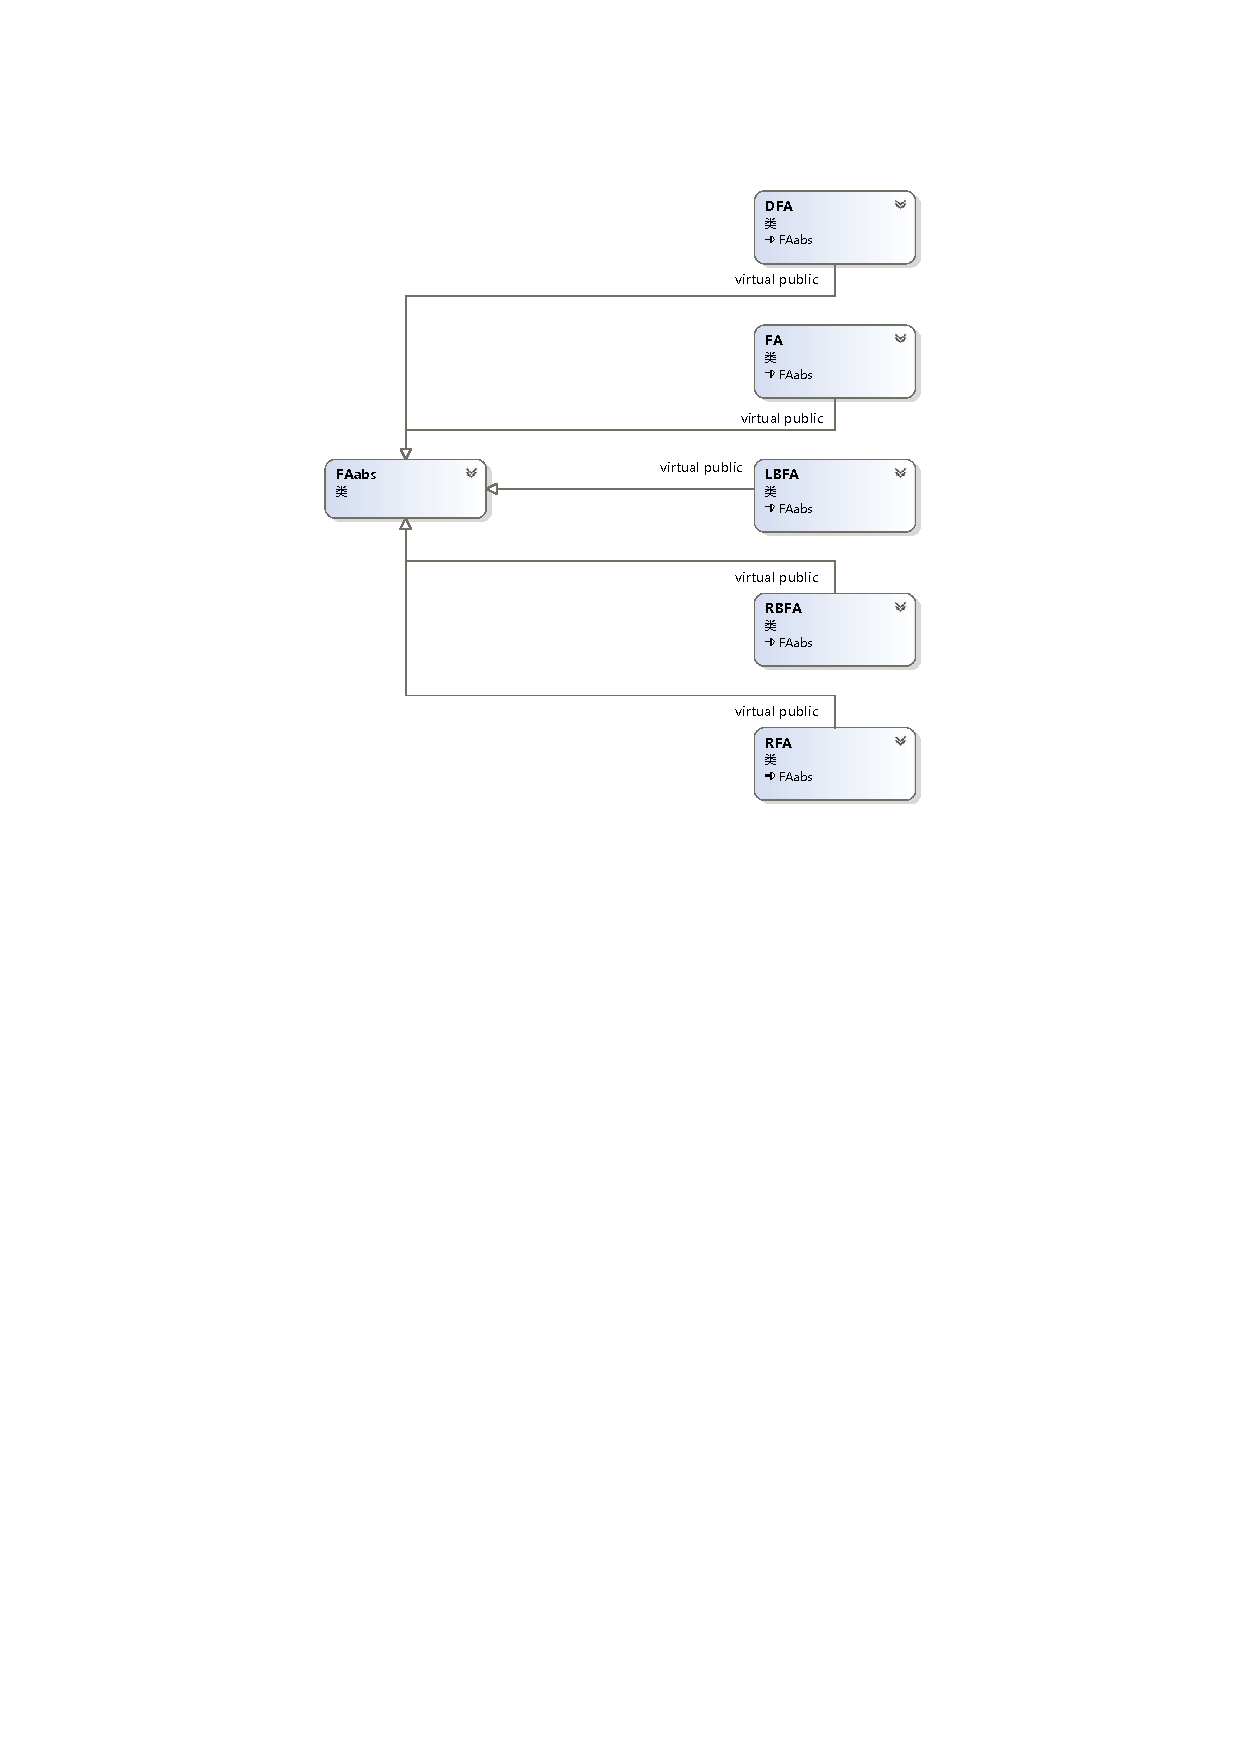
\includegraphics[width=0.7\textwidth]{FAabsRel}
    \caption{类FAabs及其派生类}
    \label{fig:FAabsRel}
\end{figure}

%\newpage
\section{DFA\_components 结构体}\label{sc:dfa_com}% ~\label{sc:dfa_com}

从“DFA\_components”构造一个$DFA$对象是最简单直接的方法,观察“DFA\_components”的实现,如表\ref{tab:DFA-components}所示
\begin{table}[!htbp]
    \caption{DFA\_components}
    \label{tab:DFA-components}
    \centering
    \small% fontsize
    \setlength{\tabcolsep}{4pt}% column separation
    \renewcommand{\arraystretch}{1.2}%row space 
    %\begin{tabular}{lcrr} 
        \begin{tabular}{p{3em}<{\centering} p{5em}<{\raggedright} p{5em}<{\raggedright}} %l p{4em}<{\centering} p{3em}<{\centering} p{3em}<{\centering}
        \toprule 
         \multicolumn{3}{c}{结构体 DFA\_components} \\
        \midrule
        名称& 类型 & \mbox{说明} \\
        \midrule
        Q & StatePool &           \\
        S & StateSet  &  $S\in Q$ \\
        F & StateSet  &  $F\in Q$ \\
        T & DTransRel &  转移关系  \\
        \bottomrule
    \end{tabular}
\end{table}
由表\ref{tab:DFA-components}可知,结构体 DFA\_components 内包含 StatePool 变量$Q$, StateSet 变量$S$, DTransRel 变量$T$, StateSet 变量$F$。若需要声明一个 DFA\_components 变量,则需要分别实例化 StatePool 、StateSet、DTransRel对象。这几个类还分别继承自其他的类,如图 \ref{fig:DFARel} 所示。

\begin{figure}[!htbp]
    \centering
    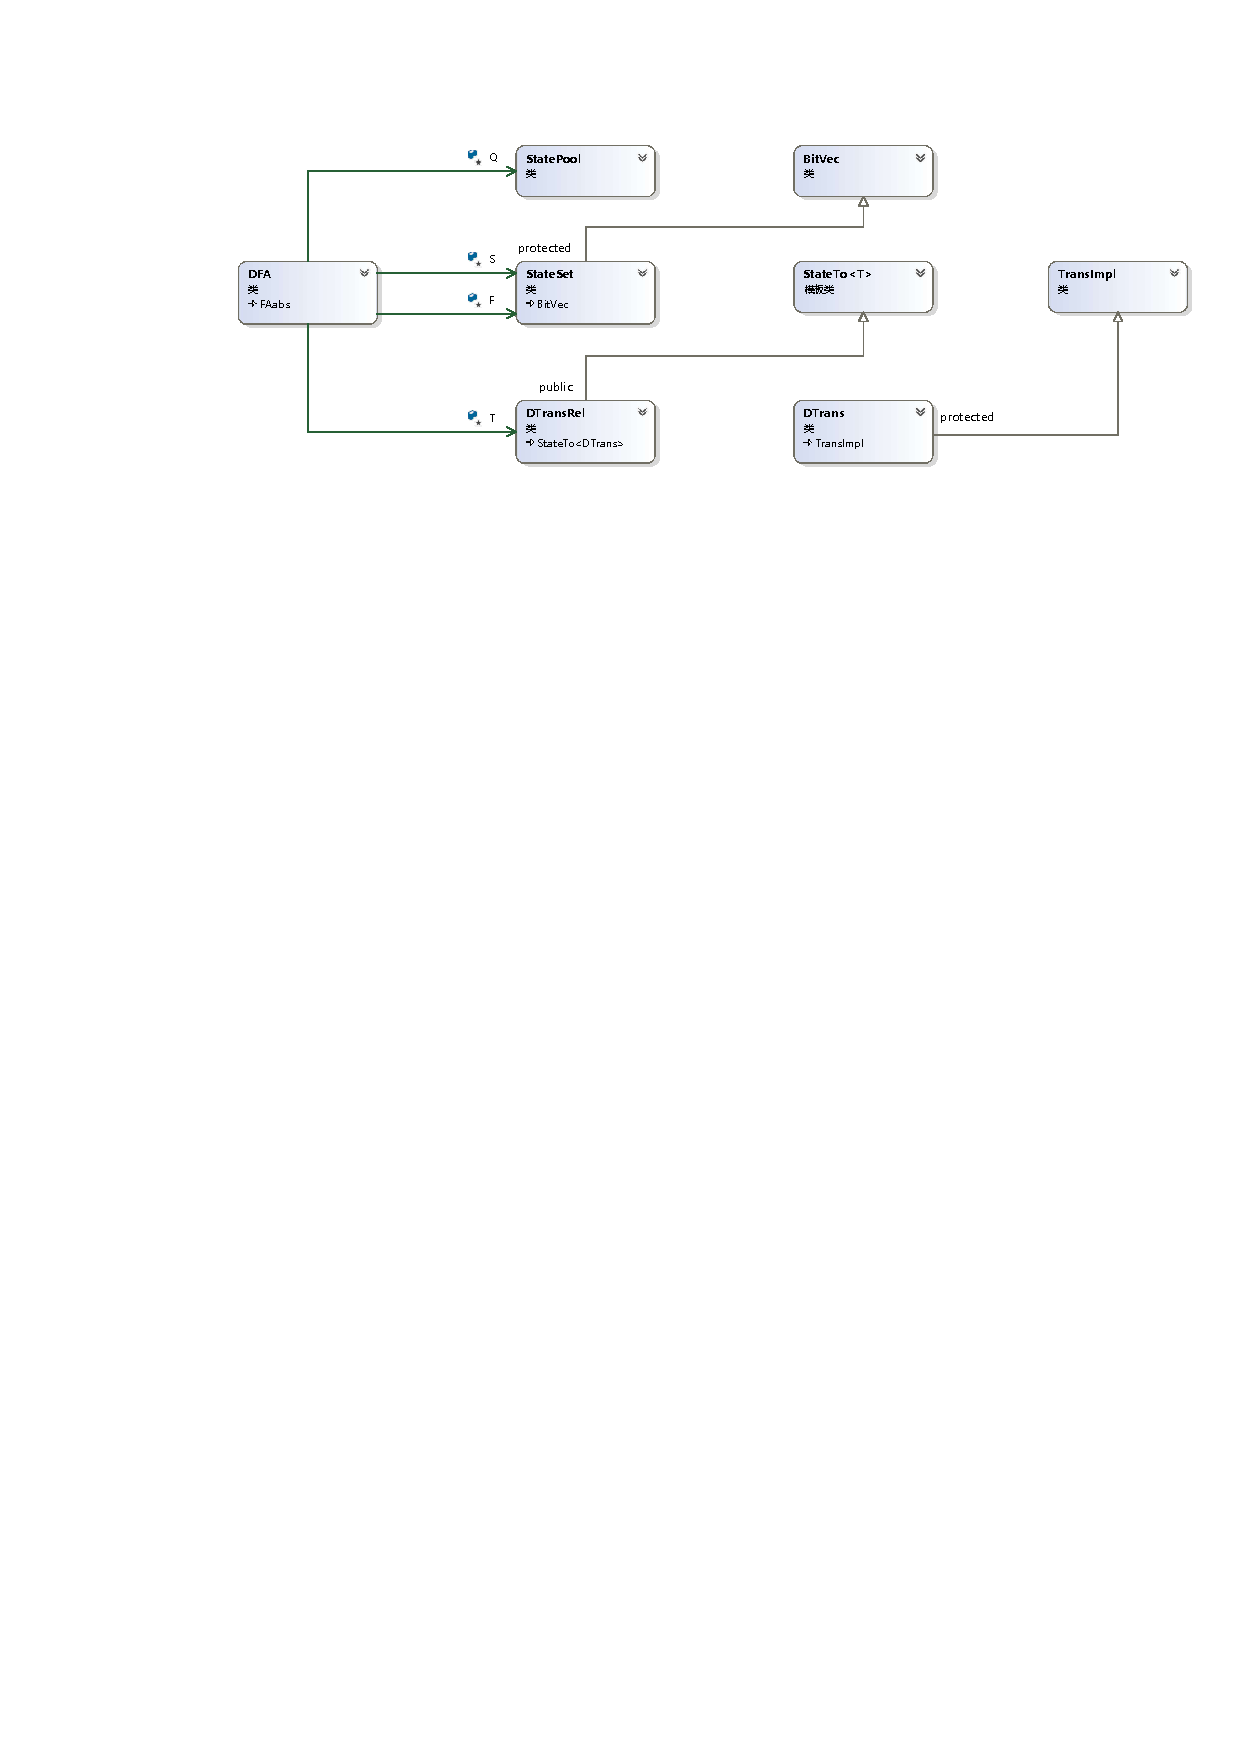
\includegraphics[width=\textwidth]{DFARel}
    \caption{DFA与其成员类及成员类的基类}
    \label{fig:DFARel}
\end{figure}

类 DFA 的成员变量 “T” 为一个 DTransRel 对象,公有继承自模板类 StateTo<T>,模板参数 “T” 为保护继承自类 TransImpl 的类 DTrans 。

\subsection{StatePool 类}
StatePool类的部分实现如表 \ref{tab:Class-StatePool} (文件$StatePool.h$):
% \lstset{style=mystyle}
% \begin{lstlisting}[language=C++,label={lst:StatePool},caption={StatePool}]
% class StatePool
% {
% public:
%     // How many states are already allocated(one more than that last allocated one,
%     // since it begins at 0).
%     inline int size() const;
%     ……
%     // Allocate a new state.
%     inline State allocate();
%     ……
% private:
%     // The next one to be allocated.
%     int next;
% };
% ……
% inline int StatePool::size() const
% {
%     return(next);
% }
% ……
% inline State StatePool::allocate()
% {
%     return(next++);
% }
% \end{lstlisting}

\begin{table}[!htbp]
    \caption{类 StatePool}
    \label{tab:Class-StatePool}
    \centering
    \small% fontsize
    \setlength{\tabcolsep}{4pt}% column separation
    \renewcommand{\arraystretch}{1.2}%row space 
    %\begin{tabular}{lcrr} 
        \begin{tabular}{llll} %l p{4em}<{\centering} p{3em}<{\centering} p{3em}<{\centering}
        \toprule 
         \multicolumn{4}{c}{Class StatePool} \\
        \midrule
        名称& 类型 & 属性  &\mbox{说明} \\
        \midrule
        next & int & private &          \\
        \midrule 
        StatePool(const StatePool\& r);& & public &构造函数 \\
        size() const; & int & public & \\
        allocate();  &   State &  public & \\
        set\_domain(const\ int r); & int & public & \\
        contains(const State r) const; & int & public & \\
        \bottomrule 
    \end{tabular}
\end{table}
如表 \ref{tab:Class-StatePool} 所示,其中 StatePool::size() 和 StatePool::allocate() 为类 StatePool 两个比较重要的函数,前者为自动机 $M$ 的大小,也即 $|M|=|Q|$。 StatePool::allocate() 用来向 StatePool 增加新的状态。
\subsection{StateSet 类}
类$StateSet$的部分声明如表 \ref{tab:Class-StateSet}(文件$StateSet.h$):
% \lstset{style=mystyle}
% \begin{lstlisting}[language=C++,label={lst:StateSet},caption={StateSet}]
% class StateSet :protected BitVec
% {
% public:
% ……
%     // inserts a State. r = [0,domain())
%     inline StateSet& add(const State r);
    
%     // set How many States can this set contain.
%     // [O, r) can be contained in *this.
%     inline void set_domain(const int r);
% ……
% }
% \end{lstlisting}

\begin{table}[!htbp]
    \caption{类 StateSet}
    \label{tab:Class-StateSet}
    \centering
    \small% fontsize
    \setlength{\tabcolsep}{4pt}% column separation
    \renewcommand{\arraystretch}{1.2}%row space 
    %\begin{tabular}{lcrr} 
        \begin{tabular}{llll} %l p{4em}<{\centering} p{3em}<{\centering} p{3em}<{\centering}
        \toprule 
         \multicolumn{4}{c}{Class StateSet : protected BitVec} \\
        \midrule
        名称& 类型 & 属性  &\mbox{说明} \\
        \midrule 
        StateSet(); &  &  public & 构造函数 \\
        empty() const; & int & public & \\
        size() const;  & int & public & \\
        complement();  & StateSet\& & public & 求补集 \\
        add(const State r);  & StateSet\& & public &  \\
        remove(const State r);  & StateSet\& & public &  \\
        set\_union(const StateSet\& r);  & StateSet\& & public & 求并集 \\
        intersection(const StateSet\& r);  & StateSet\& & public & 求交集 \\
        remove(const StateSet\& r);  & StateSet\& & public &  \\
        smallest() const; & State & public & \\
        set\_domain(const int r); & void & public & \\
        \bottomrule 
    \end{tabular}
\end{table}

由于在实例化过程$DFA$对象的过程中,只需要用到类 StateSet 的成员函数 StateSet::set\_domain() 和 StateSet::add() 。类 StateSet 中有集合的交、并、差、补、判断是否为空集等功能,这些功能实际上由类 State 的父类 BitVec 提供,这里不再赘述类 BitVec 的内容。


\subsection{DTransRel 类}

类$DTransRel$是$DFA$的一个重要成员,它存储了$DFA$的状态转移关系,最小化算法中用到的等价类分割、等价状态合并等功能都与这个类息息相关。类 DTransRel 的部分实现如表 tab:Class-DTransRel 所示(文件$DTransRel.h$):
% \lstset{style=mystyle}
% \begin{lstlisting}[language=C++,label={lst:DTransRel},caption={DTransRel}]
% // Implement a deterministic transition relation, as a function from States time
% // char to State.This is used for transition relations in DFA's.
% class DTransRel :public StateTo<DTrans>
% {
% public:
% ……
%     // Some functions updating *this:
%     inline DTransRel& add_transition(const State p, const CharRange a, const State q);
% ……
%     // Change the domain of this relation.
%     inline void set_domain(const int r);
% ……
% }
% \end{lstlisting}

\begin{table}[!htbp]
    \caption{类 DTransRel}
    \label{tab:Class-DTransRel}
    \centering
    \small% fontsize
    \setlength{\tabcolsep}{4pt}% column separation
    \renewcommand{\arraystretch}{1.2}%row space 
    %\begin{tabular}{lcrr} 
        \begin{tabular}{llll} %l p{4em}<{\centering} p{3em}<{\centering} p{3em}<{\centering}
        \toprule 
         \multicolumn{4}{c}{class DTransRel :public StateTo<DTrans>} \\
        \midrule
        名称& 类型 & 属性  &\mbox{说明} \\
        \midrule 
        DTransRel(); &  &  public & 构造函数 \\
        image(const State r, const char a) const; & State & public & \\
        transition\_on\_range(State r, CharRange a) const; & State & public & \\
        reverse\_transition(const State r, const CharRange a) const; & StateSet & public & \\
        labels\_between(const State r, const StateSet\& s) const; & CRSet & public & \\
        out\_labels(const State r) const; & CRSet & public & \\
        reverse\_closure(const StateSet\& r) const; & StateSet & public & \\
        add\_transition(State p, CharRange a, State q); & DTransRel\& & public & \\
        set\_domain(const int r); & void & public & \\
        \bottomrule 
    \end{tabular}
\end{table}

在实例化类 DFA 的过程中,类 DTransRel 需要用到的成员函数只有 DTransRel::set\_domain() 和 DTransRel::add\_transition() 。







%%%%%%%%%%%%%%%%%%%%%%%%%%%%%%%%%%%%%%%%%%%%%%%%%%%%%%%%%%%%%%%%%%%%%%%%%%%%%%%%%%%%%%%%%%%%%%%%%%%%%%%%%%%%%%%%%%%%%%
\section{实例化类DFA对象}\label{sec:get_a_dfa}

在文件$DFA.cpp$中有如下实现:
\lstset{style=mystyle}
\begin{lstlisting}[language=C++,label={lst:DFACpp},caption={DFA.cpp}]
inline int DFA::class_invariant() const
{
	return(Q.size() == S.domain()
		&& Q.size() == F.domain()
		&& Q.size() == T.domain()
		&& current < Q.size()
		&& S.size() <= 1);
}
\end{lstlisting}
而文件$DFA.h$中的构造函数如下:
\lstset{style=mystyle}
\begin{lstlisting}[language=C++,label={lst:DFA_H},caption={DFA.h}]
inline DFA::DFA(const DFA_components& r) :Q(r.Q), S(r.S), F(r.F), T(r.T)
{
	current = Invalid;
	assert(class_invariant());
}
\end{lstlisting}
由代码 \ref{lst:DFACpp} 和代码 \ref{lst:DFA_H} 可知,在语句 “assert(class\_invariant());” 处,若函数 “class\_invariant()” 返回值为 “false”,那么程序将在此处中止\cite{assert_abort}(下称 assert 中止)。由此可以知道,类$DFA$要求其成员变量满足
\begin{equation}\label{eq:DFA_class_invariant}
    (Q.size() \equiv S.domain() \equiv T.domain ) \land (S.size() \leq 1)
\end{equation}
对于$current \le Q.size() $,“current”变量的值被初始化为“Invalid”,并且之后没有对其进行更改,所以不列入式\ref{eq:DFA_class_invariant}中。

在文件$State.h$中有如下定义
\lstset{style=mystyle}
\begin{lstlisting}[language=C++,label={lst:State_H},caption={State.h}]
// Encode automata states as integers.
typedef signed int State;

// Invalid states mean something bad is about to happen.
const State Invalid = -1;
\end{lstlisting}
由代码\ref{lst:State_H}可知,$State$类型实际上是整型,而“Invalid”为“-1”。

%\clearpage
根据本节以上内容以及\ref{sc:dfa_com}节内容所说,可以实例化如图\ref{fig:DFA1}的自动机。

\begin{figure}[!htbp]
    \centering
    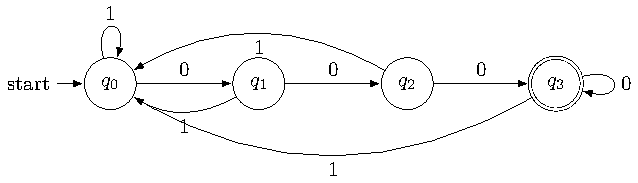
\includegraphics[width=0.7\textwidth]{automaton_1}
    \caption{DFA示例}
    \label{fig:DFA1}
\end{figure}

\newpage
图\ref{fig:DFA1}中的自动机的转移函数如表\ref{tab:DFA1}

\begin{table}[!htbp]
    \caption{图{\ref{fig:DFA1}}状态转移函数}
    \label{tab:DFA1}
    \centering
    \small% fontsize
    \setlength{\tabcolsep}{4pt}% column separation
    \renewcommand{\arraystretch}{1.2}%row space 
    \begin{tabular}{l p{3em}<{\centering} p{3em}<{\centering} p{3em}<{\centering}}
        \toprule %\hline 
        \multirow{2}{*}{状态说明} & \multirow{2}{*}{状态} & \multicolumn{2}{c}{输入字符} \\
		\cline{3-4}      &    &$0$ & $1$  \\
        \midrule%\hline
        开始状态(start)          & $q_0$ & $q_1$  & $q_0$    \\
                                & $q_1$ & $q_2$  & $q_0$    \\
                                & $q_2$ & $q_3$  & $q_0$    \\
        结束状态(final)         & $q_3$ & $q_3$  & $q_0$    \\
        \bottomrule%\hline  
    \end{tabular}
\end{table}

实例化$DFA$类如代码\ref{lst:DFASample}:

% \lstset{style=mystyle}
% \begin{lstlisting}[language=C++,label={lst:DFASample},caption={实例化DFA示例}]
% #include"DFA.h"
% #include<iostream>
% int main()
% {
%     DFA_components dfa_com1;

%     // StateSet S  开始状态集
%     dfa_com1.S.set_domain(10);
%     dfa_com1.S.add(0);

%     // StateSet F  结束状态集
%     dfa_com1.F.set_domain(10);
%     dfa_com1.F.add(3);

%     // StatePool Q 
%     int i = 10;
%     while (i--)
%     {
%         dfa_com1.Q.allocate();
%     }

%     // DTransRel T transition             
%     dfa_com1.T.set_domain(10);
%     dfa_com1.T.add_transition(0, '0', 1);
%     dfa_com1.T.add_transition(1, '0', 2);
%     dfa_com1.T.add_transition(2, '0', 3);
%     dfa_com1.T.add_transition(3, '0', 3);
%     dfa_com1.T.add_transition(0, '1', 0);
%     dfa_com1.T.add_transition(1, '1', 0);
%     dfa_com1.T.add_transition(2, '1', 0);
%     dfa_com1.T.add_transition(3, '1', 0);

%     DFA dfa1(dfa_com1);
%     dfa1.usefulf();

%     std::cout<<dfa1<<std::endl;
	
%     return 0;
% }
% \end{lstlisting}

代码 \ref{lst:DFASample} 将在控制台输出如下信息:
\lstset{style=mystyle}
\begin{lstlisting}[language=C++,label={lst:DFASampleLog},caption={图\ref{fig:DFA1}中自动机在 FIRE engine 中的表现形式}]
DFA
Q = [0,4)
S = { 0 }
F = { 3 }
Transitions =
0->{ '0'->1  '1'->0 }
1->{ '0'->2  '1'->0 }
2->{ '0'->3  '1'->0 }
3->{ '0'->3  '1'->0 }

current = -1
\end{lstlisting}

下文中将以表\ref{tab:DFA1}的形式来描述一个自动机,以代码\ref{lst:DFASampleLog}的形式来表示自动机在 FIRE engine 中的展现形式。实例化一个 DFA 时以 “实例化 DFA” 代指,不用代码表示。 
%!TEX root = ../Demo.tex
\chapter{测试内容}\label{cha:realwork}

本章内容为测试结果、测试过程中发现的问题、以及如何修复(部分)这些问题。

% \begin{remark}
%     因为$DFA$的最小化建立在状态等价性的基础之上,所以本文并未专门针对等价性进行测试。    
% \end{remark}
%%%%%%%%%%%%%%%%%%%%%%%%%%%%%%%%%%%%%%%%%%%%%%%%%%%%%%%%%%%%%%%%%%%%%%%%%%%%%%%%%%%%%%%%%%%%%%%%%%%%%%%%%%%%%%%%%%%%%%%%%%%%%%%%%%%%%%%%%%%%%%%%%
\section{如何测试}









%%%%%%%%%%%%%%%%%%%%%%%%%%%%%%%%%%%%%%%%%%%%%%%%%%%%%%%%%%%%%%%%%%%%%%%%%%%%%%%%%%%%%%%%%%%%%%%%%%%%%%%%%%%%%%%%%%%%%%%%%%%%%%%%%%%%%%%%%%%%%%%%%
\section{无限循环}\label{sec:ohloop}

实例化一个如表 \ref{tab:DFA4} 的 DFA 的对象之后,调用函数 DFA::min\_Watson()。(表 \ref{tab:DFA4} 对应的状态转移图为图 \ref{fig:DFA4_0},含有陷阱状态 $q_5$ \footnote{进入此状态之后无法通过任何转移离开,如图 \ref{fig:DFA4_0} 中的状态 {$q_5$}。} )

\begin{table}[!htbp]
    \caption{接受{$\mathcal{L}=0^*10^*$}的自动机{\cite{book1}}}
    \label{tab:DFA4}
    \centering
    \small% fontsize
    \setlength{\tabcolsep}{4pt}% column separation
    \renewcommand{\arraystretch}{1.2}%row space 
    %\begin{tabular}{lcrr} 
        \begin{tabular}{l p{3em}<{\centering} p{3em}<{\centering} p{3em}<{\centering}}
        \toprule %\hline 
        \multirow{2}{*}{状态说明} & \multirow{2}{*}{状态} & \multicolumn{2}{c}{输入字符} \\
		\cline{3-4}      &    &$0$ & $1$  \\
        \midrule%\hline
        开始状态(start)  & $q_0$ & $q_1$   & $q_2$   \\
                        & $q_1$ & $q_0$   & $q_3$   \\
        结束状态(final) & $q_2$ & $q_4$   & $q_5$   \\
        结束状态(final) & $q_3$ & $q_4$   & $q_5$   \\
        结束状态(final) & $q_4$ & $q_4$   & $q_5$   \\
        陷阱状态(sink) & $q_5$ & $q_5$   & $q_5$   \\
        \bottomrule%\hline 
    \end{tabular}
\end{table}

% {\bfseries 运行结果:} 函数进入无限循环
\subsection{运行结果}
函数进入无限循环。

% {\bfseries 错误原因:}
\subsection{错误原因} 

单步调试发现进入无限循环的位置为min-bww.cpp(124行),为代码 \ref{lst:minbww} 中的“H.equivalize(p, q);”。
\lstset{style=mystyle}
\begin{lstlisting}[language=C++,label={lst:minbww},caption={min-bww.cpp}]
if (are_eq(p, q, S, H, Z))
{
    // p and q are equivalent.
    H.equivalize(p, q);
}
\end{lstlisting}
单步进入该函数,可以看到代码 \ref{lst:StateEqRel} (StateEqRel.cpp(42行))
\lstset{style=mystyle}
\begin{lstlisting}[language=C++,label={lst:StateEqRel},caption={StateEqRel.cpp}]
for (oldq->iter_start(i); !oldq->iter_end(i); oldq->iter_end(i))
{
    map(i) = newp;
}
\end{lstlisting}
for循环的一般格式如代码 \ref{lst:for}
\lstset{style=mystyle}
\begin{lstlisting}[language=C++,label={lst:for},caption={for 循环的一般格式}]
for (初始化循环变量; 循环条件; 迭代)
{
    循环体
}
\end{lstlisting}
在代码 \ref{lst:StateEqRel} 中循环变量为“i”,循环条件为“!oldq->iter\_end(i);”,迭代为“oldq->iter\_end(i)”。查看“iter\_end()”函数实现如代码 \ref{lst:itend}
\lstset{style=mystyle}
\begin{lstlisting}[language=C++,label={lst:itend},caption={函数 iter\_end() 的实现}]
// StateSet.h
// Is r the last State in an iteration sequence.
inline int StateSet::iter_end(State r) const
{
	return(BitVec::iter_end(r));
}

// BitVec.h
// Is r the last set bit in an iteration sequence.
// if (r== -1) retrun 1; else return 0
inline int BitVec::iter_end(int r) const
{
	return(r == -1);
}
\end{lstlisting}
可以看到函数“iter\_end()”并未对参数“i”进行更改。于是程序在此处进入无限循环。

% {\bfseries 解决方法} :
\subsection{解决方法}

将代码 \ref{lst:StateEqRel} 中的迭代 “oldq->iter\_end(i)” 更改为 “oldq->iter\_next(i)”,更改后如代码 \ref{lst:StateEqRel2} ,经过比对,更改后与原文 \cite{watson1994design} 相同。
\lstset{style=mystyle}
\begin{lstlisting}[language=C++,label={lst:StateEqRel2},caption={StateEqRel.cpp}]
for (oldq->iter_start(i); !oldq->iter_end(i); oldq->iter_next(i))
{
    map(i) = newp;
}
\end{lstlisting}

{\bfseries 更改后}:函数“DFA::min\_Watson();”不再陷入无限循环。


%%%%%%%%%%%%%%%%%%%%%%%%%%%%%%%%%%%%%%%%%%%%%%%%%%%%%%%%%%%%%%%%%%%%%%%%%%%%%%%%%%%%%%%%%%%%%%%%%%%%%%%%%%%%%%%%%%%%%%%%%%%%%%%%%%%%%%%%%%%%%%%%%
%%%%%%%%%%%%%%%%%%%%%%%%%%%%%%%%%%%%%%%%%%%%%%%%%%%%%%%%%%%%%%%%%%%%%%%%%%%%%%%%%%%%%%%%%%%%%%%%%%%%%%%%%%%%%%%%%%%%%%%%%%%%%%%%%%%%%%%%%%%%%%%%%
\section{函数 DFA::usefulf() 运行错误}\label{sec:usefulf}

“DFA::usefulf()” 函数为一个重要函数。用于去除有限自动机中的非 “final-reachable” 状态,在执行最小化算法前执行该函数,可以去除有限自动机中的非“final-reachable”状态,进而减少程序运行时间。其定义如代码 \ref{lst:usefulf}
\lstset{style=mystyle}
\begin{lstlisting}[language=C++,label={lst:usefulf},caption={DFA::usefulf()}]
// Remove any States that cannot reach a final State.
// (This is a last step in minimization, since some of the min. algorithms may yield a DFA with a sink state.)
// Implement Remark 2.39  removing states that are not final - reachable.
DFA& usefulf();
\end{lstlisting}
以图 \ref{fig:DFA4_0} 为例,状态$q_5$ 即为非 “final-reachable” 状态(下称陷阱状态)。移除状态 $q_5$ 之后如图 \ref{fig:DFA4_1} 。图 \ref{fig:DFA4_1} 转移函数如表 \ref{tab:DFA4_1}。

\begin{table}[!htbp]
    \caption{接受{$\mathcal{L}=0^*10^*$}的自动机{\cite{book1}}}
    \label{tab:DFA4_1}
    \centering
    \small% fontsize
    \setlength{\tabcolsep}{4pt}% column separation
    \renewcommand{\arraystretch}{1.2}%row space 
    %\begin{tabular}{lcrr} 
        \begin{tabular}{l p{4em}<{\centering} p{3em}<{\centering} p{3em}<{\centering}}
        \toprule %\hline 
        \multirow{2}{*}{状态说明} & \multirow{2}{*}{状态} & \multicolumn{2}{c}{输入字符} \\
		\cline{3-4}      &    &$0$ & $1$  \\
        \midrule%\hline
        开始状态(start)  & $q_0$ & $q_1$   & $q_2$   \\
                        & $q_1$ & $q_0$   & $q_3$   \\
        结束状态(final) & $q_2$ & $q_4$   & -   \\
        结束状态(final) & $q_3$ & $q_4$   & -   \\
        结束状态(final) & $q_4$ & $q_4$   & -   \\
        \bottomrule%\hline 
    \end{tabular}
\end{table}

%%%%%%%%%%%%%%%%%%%%%%%%%%%%%%%%%%%%%%%%%%%%%%%%%%%%%%%%%%%%%%%%%%%%%%%%%%%%%%%%%%%%%%%%%%%%%%%%%%%%%%%%%%%%%%%%%%%%%%%%%%%%%%
% {\bfseries 运行结果}
\subsection{运行结果}

执行函数“DFA::usefulf()”后若状态 $q_5$ 被去除,则函数定义功能正常执行。但是在实际的执行过程中,程序提示如图 \ref{fig::usefulf_error} 错误 

\begin{figure}[!htbp]
    \centering
    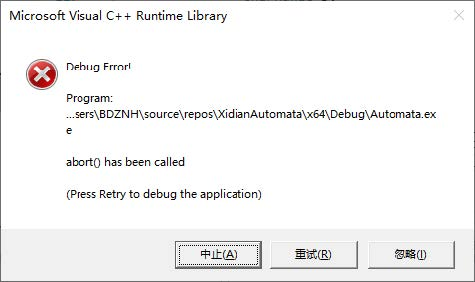
\includegraphics[width=0.60\textwidth]{DFA_usefulf_error}
    \caption{函数 DFA::usefulf() 错误提示}
    \label{fig::usefulf_error}
\end{figure}
控制台提示如图 \ref{fig::usefulf_console_log}
\begin{figure}[!htbp]
    \centering
    %trim option's parameter order: left bottom right top
    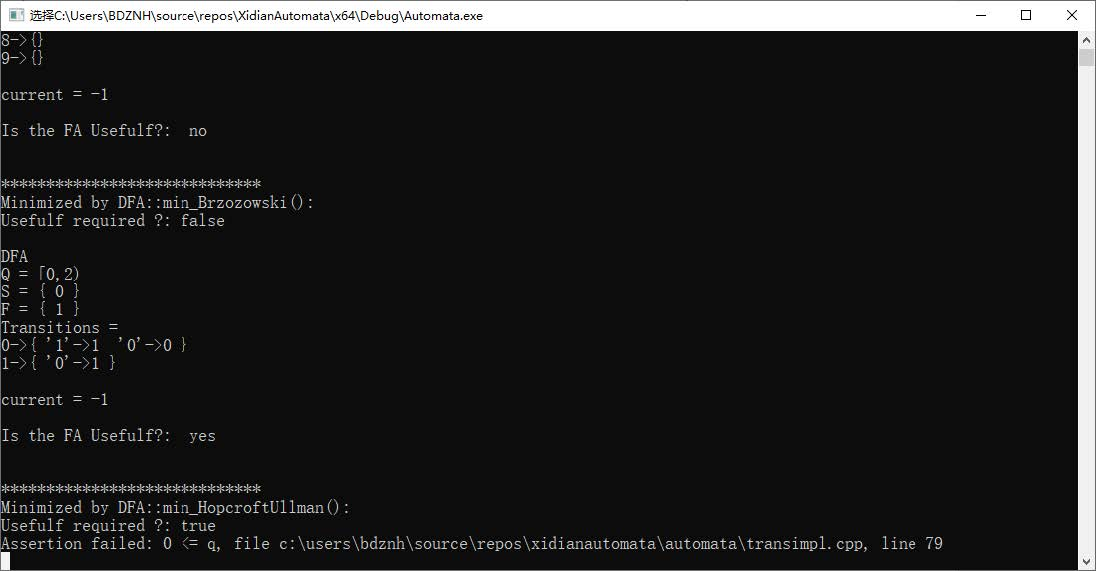
\includegraphics[trim = 0mm 0mm 0mm 63mm, clip,width=0.95\textwidth]{DFA_usefulf_console_log}
    \caption{函数 DFA::usefulf() 错误提示}
    \label{fig::usefulf_console_log}
\end{figure}

可以确定函数未完成其定义功能。

%%%%%%%%%%%%%%%%%%%%%%%%%%%%%%%%%%%%%%%%%%%%%%%%%%%%%%%%%%%%%%%%%%%%%%%%%%%%%%%%%%%%%%%%%%%%%%%%%%%%%%%%%%%%%%%%%%%%%%%%%%%%%%%%%%%%%%%%%%%%%%%%%%%%%%%%%%%%%%%%%%%%%%%%%%%%%
% {\bfseries 错误原因}
\subsection{错误原因}

查看 TransImple.cpp,79行,代码如下
\lstset{style=mystyle}
\begin{lstlisting}[language=C++,label={lst:TransImple},caption={ TransImple.cpp },firstnumber=75]
// Add a transition to the set.
TransImpl& TransImpl::add_transition(const CharRange a, const State q)
{
    assert(a.class_invariant());
    assert(0 <= q);
    ………
}
\end{lstlisting}

在 79 行处打断点,单步调试至此处,可以看到 State 变量 q 的值为“-842150451”,对应的十六进制值为“0xFFFFFFFF”\footnote{调试时使用 64 位编译器产生的二进制文件,在 64 位系统下运行。},为常见的未初始化错误。此时表达式 “0 <= q” 不成立,返回值为 “false” , 程序在此处中止。

查看函数 DFA::usefulf() 的实现,如代码 \ref{lst:DFA_usefulf_1} 。
\lstset{style=mystyle}
\begin{lstlisting}[language=C++,label={lst:DFA_usefulf_1},caption={ DFA.cpp },firstnumber=84]
StateTo<State> newnames;
newnames.set_domain(Q.size());

// All components will be constructed into a special structure :
DFA_components ret;
State st;
for (st = 0; st < Q.size(); st++)
{
    // If this is a Usefulf State, carry it over by giving it a name
    // in the new DFA.
    if (freachable.contains(st))
    {
        newnames.map(st) = ret.Q.allocate();
    }
}
\end{lstlisting}
在代码 \ref{lst:DFA_usefulf_1} 中将 “ final-reachable ” 状态保存到 StateTo<State> 变量 newnames 中,通过 “ ret.Q.allocate()” 为状态命名新的状态名,作为新的自动机的状态名。DFA\_components 变量 ret 用于构建新的自动机,再看函数内构造新的自动机的主要实现部分,如代码 \ref{lst:DFA_usefulf_2}
\lstset{style=mystyle}
\begin{lstlisting}[language=C++,label={lst:DFA_usefulf_2},caption={ DFA.cpp },firstnumber=130]
for (it = 0; !a.iter_end(it); it++)
{
    b = a.iterator(it);
    ret.T.add_transition(stprime, b, newnames.lookup(T.transition_on_range(st, b)));
}
\end{lstlisting}

根据代码 \ref{lst:TransImple} ,可以知道程序中止的地方为代码 \ref{lst:DFA_usefulf_2},133 行。其中 State 变量为当前需要进行操作的状态,CharRange 变量 b 为当前状态转移输入字符。查看 T.
transition\_on\_range(st, b)) 的实现,如代码 \ref{lst:transition_on_range}
\lstset{style=mystyle}
\begin{lstlisting}[language=C++,label={lst:transition_on_range},caption={ DTransRel.cpp },firstnumber=108]
// Compute the image of r, and CharRange it under *this.
inline State DTransRel::transition_on_range(const State r, const CharRange a) const
{
    assert(class_invariant());
    assert(0 <= r && r < domain());
    return(lookup(r).range_transition(a));
}
\end{lstlisting}
由代码 \ref{lst:transition_on_range} 可知,T.transition\_on\_range(st, b)) 将返回原自动机中,状态 st 经过输入字符 b 转移之后的目标状态。

查看 newnames.lookup() 的实现,如代码 \ref{lst:newnames-lookup}
\lstset{style=mystyle}
\begin{lstlisting}[language=C++,label={lst:newnames-lookup},caption={ StateTo.h },firstnumber=177]
// The actual mapping function
// First, a const lookup operator.
template<class T>
inline const T& StateTo<T>::lookup(const State r) const
{
    assert(class_invariant());
    // First check that it's in bounds
    assert(0 <= r && r < domain());
    return(data[r]);
}
\end{lstlisting}
在本例中,模板类 StateTo<T> 的模板参数 “T” 为 State。则 newnames.lookup(T.transition\_on\_range(st, b)) 为原自动机中 状态 st 经过字符 b 转移后的目标状态在新自动机中的状态。然后通过 ret.T.add\_transition() 保存新的转移关系。对所有的状态进行以上操作之后,通过变量 ret 构造新的自动机。 

经过单步调试发现,表\ref{tab:DFA4} 中,状态 $q_2$ 经过字符 “1” 将转移到状态 $q_5$,而在代码 \ref{lst:DFA_usefulf_1} 中,状态 $q_5$ 不满足 “if (freachable.contains(st))”,所以状态 $q_5$ 未被新的自动机保存,进而在代码 \ref{lst:DFA_usefulf_2} 中,当 st 为状态 $q_2$ 且 b 为字符 “1” 时,“newnames.lookup(T.transition\_on\_range(st, b))” 将返回未经初始化的值“-842150451”,于是在代码 \ref{lst:TransImple} 中,State 变量 q 的值为“-842150451”,导致程序在此处中止。

%%%%%%%%%%%%%%%%%%%%%%%%%%%%%%%%%%%%%%%%%%%%%%%%%%%%%%%%%%%%%%%%%%%%%%%%%%%%%%%%%%%%%%%%%%%%%%%%%%%%%%%%%%%%%%%%%%%%%%%%
\subsection{解决方法}

如代码 \ref{lst:State_H} 所示,文件 State.h 中将无效状态设置为 “Invalid”。在代码 \ref{lst:DFA_usefulf_1}增加处理不满足条件 “freachable.contains(st)” 的状态的内容,将原自动机中的非“final-reachable”状态标记为 “Invalid”,更改后为代码 \ref{lst:DFA_usefulf_1_edit}
\lstset{style=mystyle}
\begin{lstlisting}[language=C++,label={lst:DFA_usefulf_1_edit},caption={ 更改后的 DFA.cpp },firstnumber=91]
for (st = 0; st < Q.size(); st++)
{
    // If this is a Usefulf State, carry it over by giving it a name
    // in the new DFA.
    if (freachable.contains(st))
    {
        newnames.map(st) = ret.Q.allocate();
    }
    else                            // 新增
    {                               // 新增
        newnames.map(st) = Invalid; // 新增
    }                               // 新增
}
\end{lstlisting}

在代码 \ref{lst:DFA_usefulf_2} 中,在添加新的转移关系之前判断当前状态和目标状态是否都是有效状态,若都为有效状态,则添加新的转移关系。更改后为代码 \ref{lst:DFA_usefulf_2_edit}
\lstset{style=mystyle}
\begin{lstlisting}[language=C++,label={lst:DFA_usefulf_2_edit},caption={ 更改后的 DFA.cpp },firstnumber=133]
    State stdest;                                           // 新增
    stdest = newnames.lookup(T.transition_on_range(st, b)); // 新增

    if (stprime != Invalid &&  stdest != Invalid)           // 新增
    {                                                       // 新增
        ret.T.add_transition(stprime, b, stdest));          // 修改
    }                                                       // 新增
\end{lstlisting}

更改后函数 DFA::usefulf() 成功移除图 \ref{fig:DFA4_0} 中的陷阱状态 $q_5$ ,将图 \ref{fig:DFA4_0} 转换成图 \ref{fig:DFA4_1}。
更改后函数 DFA::usefulf() 成功移除图 \ref{fig:usefulf2-1} 中的陷阱状态 $q_1$ ,将图 \ref{fig:usefulf2-1} 转换成图 \ref{fig:usefulf2-2} 。



%%%%%%%%%%%%%%%%%%%%%%%%%%%%%%%%%%%%%%%%%%%%%%%%%%%%%%%%%%%%%%%%%%%%%%%%%%%%%%%%%%%%%%%%%%%%%%%%%%%%%%%%%%%%%%%%%%%%%%%%%%%%%%%%%%%%%%%%%%%%%%%%%%%%%%%%%%
%%%%%%%%%%%%%%%%%%%%%%%%%%%%%%%%%%%%%%%%%%%%%%%%%%%%%%%%%%%%%%%%%%%%%%%%%%%%%%%%%%%%%%%%%%%%%%%%%%%%%%%%%%%%%%%%%%%%%%%%%%%%%%%%%%%%%%%%%%%%%%%%%%%%%%%%%%
\section{函数 DFA::min\_Hopcroft() 运行错误}\label{sec:hopcroft}

% Hopcroft 算法描述如下\cite{watson1993taxonomyb} \\
% {\small \setlength{\parskip}{1em}
% \rule{\textwidth}{1pt}
% \mbox{ } $P:=[Q]_{E_0}$; \\
% \mbox{ } $L:= ( \mbox{\textbf{if }} ( |F| \leq |Q \setminus F | ) \mbox{\textbf{then }} \{F\} \mbox{\textbf{else }} \{ Q \setminus F \} \mbox{\textbf{fi }} ) \times V $; \\
% \mbox{ } $ \{ \mbox{恒有: } [Q]_E \sqsubseteq P \sqsubseteq [Q]_{E_0} \land L \subseteq (P \times V) $ \\
% \mbox{   } $ \land (\forall Q_0,Q_1,a:Q_0 \in Q \land (Q_1,a) \in L : \neg Splittable (Q_0,Q_1,a)) \Rightarrow (P=[Q]_E) \} $ \\
% \mbox{ } $ \mbox{\textbf{do }} L \not= \emptyset \longrightarrow $ \\ 
% \mbox{   } $ \mbox{\textbf{let }} Q_1,a:(Q_1,a) \in L $; \\
% \mbox{   } $ P_{old} := P $; \\
% \mbox{   } $ L := L \setminus \{ (Q_1,a) \} $; \\
% \mbox{   } $ \{  \mbox{恒有: } [Q]_E \sqsubseteq P \sqsubseteq P_{old} \} $ \\
% \mbox{   } $ \mbox{\textbf{for }} Q_0 : Q_0 \in P_{old} \land Splittable (Q_0,Q_1,a) \mbox{\textbf{ do }} $ \\
% \mbox{     } $ Q'_0 := \{ p:p \in Q_0 \land T(p,a) \in Q_1 \} $; \\
% \mbox{     } $ P:= P \setminus \{ Q_0 \} \cup \{ Q_0 \setminus Q'_0,b \} $;\\
% \mbox{     } $ \mbox{\textbf{for }} b:b \in V \mbox{\textbf{ do }} $ \\
% \mbox{       } $ \mbox{\textbf{if }} (Q_0,b) \in L \rightarrow L := L \setminus \{ (Q_0,b) \} \cup \{ (Q'_0,b),(Q_0, \setminus Q'_0,b ) \} $;\\ 
% \mbox{       } $ \talloblong (Q_0,b) \notin L \rightarrow $ \\
% \mbox{         } $ L := L \cup (\mbox{\bfseries if} ( |Q'_0| \leq |Q_0 \setminus Q'_0| ) \mbox{\bfseries then} \{ (Q'_0 , b) \} \mbox{\bfseries else} \{ ( Q'_0 \setminus Q'_0,b ) \} \mbox{\bfseries fi} ) $ \\
% \mbox{       } $ \mbox{\textbf{fi}} $ \\
% \mbox{     } $ \mbox{\textbf{rof}} $ \\
% \mbox{   } $ \mbox{\textbf{rof}} $ \\
% \mbox{   } $ \{ (\forall Q_0,Q_0 \in P : \neg Splittable(Q_0,Q_1,a)) \} $ \\
% \mbox{ } $ \mbox{\textbf{od }} \{ P = [Q]_E \} $ \\
% \rule{\textwidth}{1pt} }

实例化如表 \ref{tab:DFA411-1} 所示的自动机。(含有开始不可达状态\footnote{从开始状态不可以到达的状态,如图 \ref{fig:DFA11-0} 中状态 $q_9$ 。}(start-unreachable))

\begin{table}[!htbp]
    \caption{图\ref{fig:DFA11-0}的转移函数}
    \label{tab:DFA411-1}
    \centering
    \small% fontsize
    \setlength{\tabcolsep}{4pt}% column separation
    \renewcommand{\arraystretch}{1.2}%row space 
    %\begin{tabular}{lcrr} 
        \begin{tabular}{l p{4em}<{\centering} p{3em}<{\centering} p{3em}<{\centering}}
        \toprule %\hline 
        \multirow{2}{*}{状态说明} & \multirow{2}{*}{状态} & \multicolumn{2}{c}{输入字符} \\
		\cline{3-4}      &    &$0$ & $1$  \\
        \midrule%\hline
        开始状态(start)  & $q_0$ & $q_1$   & $q_2$   \\
                        & $q_1$ & $q_5$   & $q_2$   \\
                        & $q_2$ & $q_3$   & $q_6$   \\
                        & $q_3$ & $q_2$   & $q_4$   \\
        结束状态(final) & $q_4$ & $q_8$   & $q_1$   \\
                        & $q_5$ & $q_1$   & $q_6$   \\
                        & $q_6$ & $q_7$   & $q_2$   \\
                        & $q_7$ & $q_6$   & $q_8$   \\
        结束状态(final) & $q_8$ & $q_5$   & $q_4$   \\
        开始不可达状态    & $q_9$ & $q_7$   & $q_5$   \\
        \bottomrule%\hline 
    \end{tabular}
\end{table}

函数 DFA::min\_Hopcroft() 是 Hopcroft 算法在 FIRE engine 中的实现,Hopcroft 算法在文中\cite{watson1993taxonomyb}描述如下:
\begin{figure}[!htbp]
    \centering
        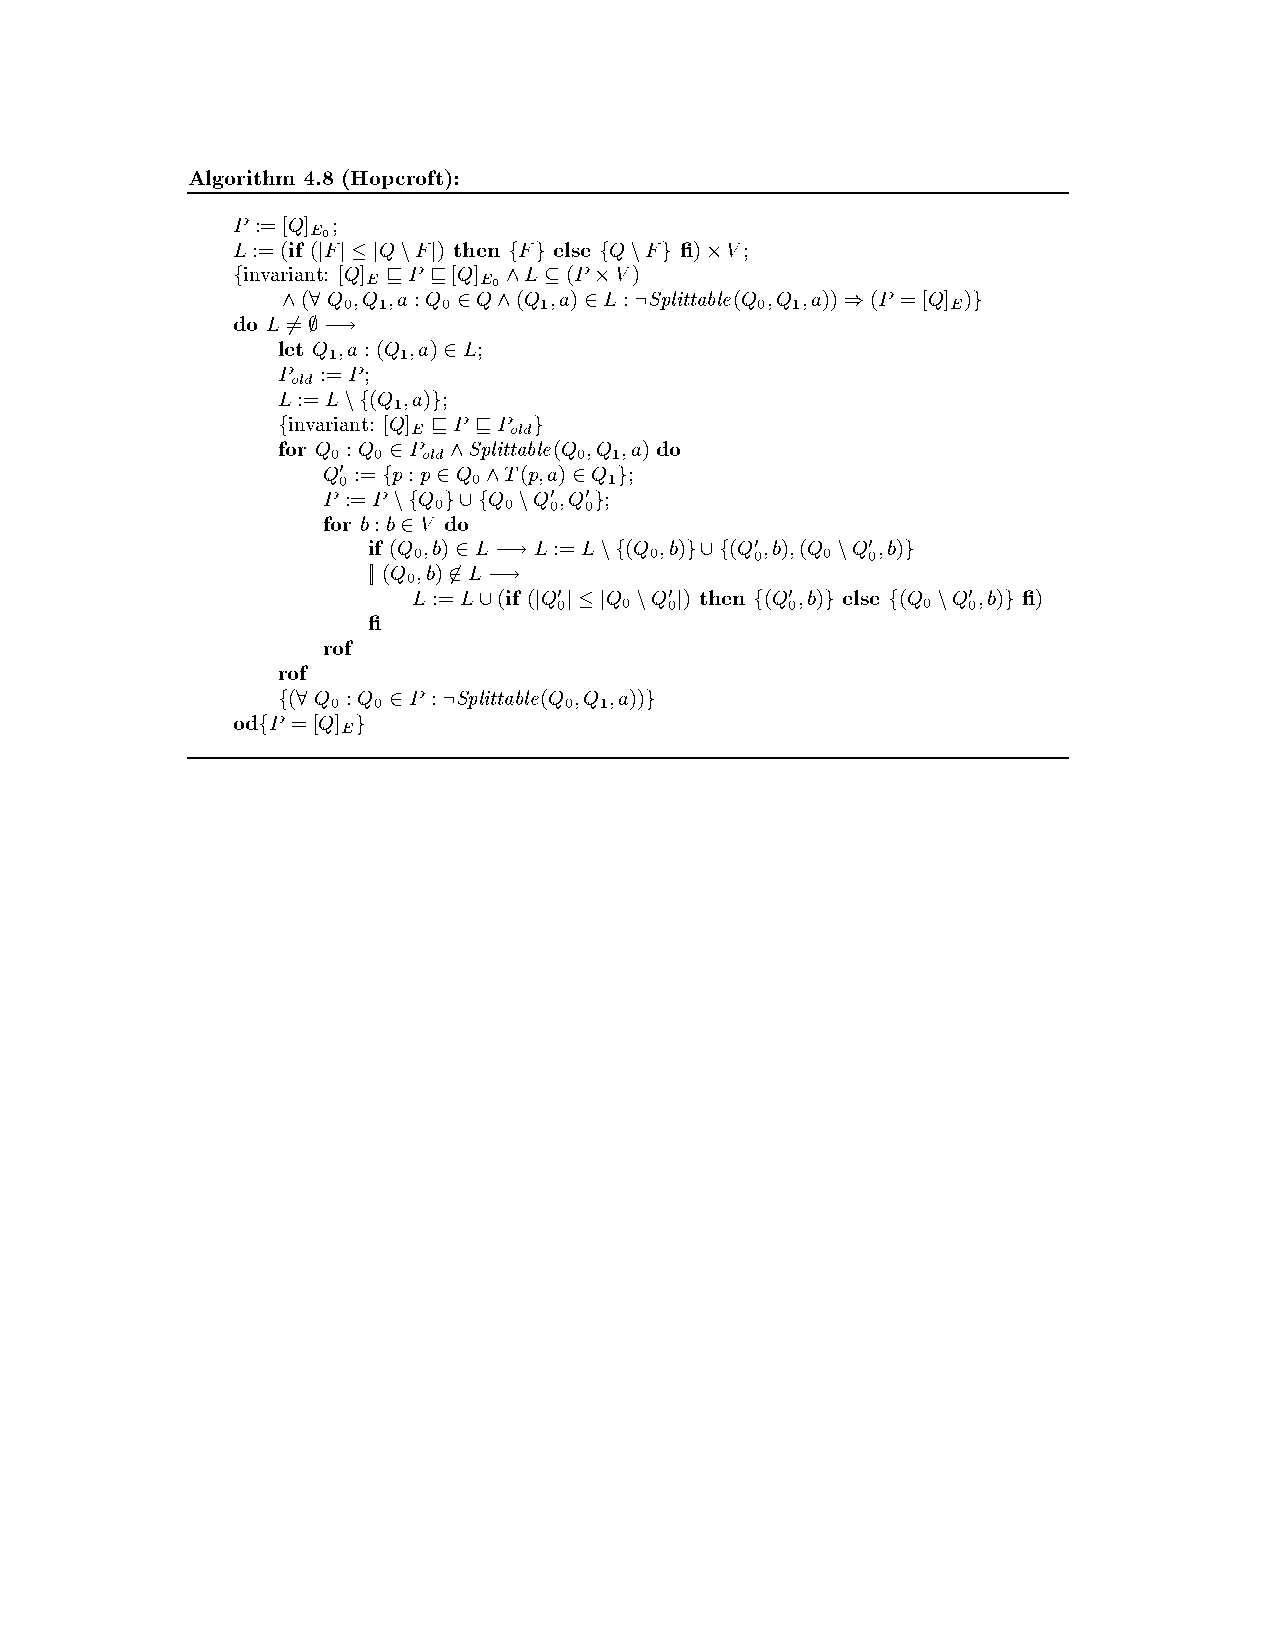
\includegraphics[width=0.99\textwidth]{hopcroft}
\end{figure}

\subsection{运行结果}\label{sec:hopcroft-error}
执行函数 DFA::min\_Hopcroft(),程序在文件CRSet.h,第 146 行的 “assert(!iter\_end(it))” 处触发 assert 中止,如代码 \ref{lst:iterend} 所示。调用函数“CRSet::iterator()”的地方为文件min-hop.cpp,第103行,“State r(split(p, q, C.iterator(L[q]), P));”的“C.iterator(L[q])”处。
\lstset{style=mystyle}
\begin{lstlisting}[language=C++,label={lst:iterend},caption={ CRSet.h },firstnumber=142]
// Fetch the it'th CharRange in *this.
inline const CharRange& CRSet::iterator(const int it) const
{
    assert(class_invariant());
    assert(!iter_end(it));
    return(data[it]);
}

// Is there even in it'th CharRange?
inline int CRSet::iter_end(const int it) const
{
    assert(class_invariant());
    assert(0 <= it);
    return(it >= in_use);
}
\end{lstlisting}

\subsection{错误原因}

以表 \ref{tab:DFA411-1} 中实例化的自动机为例,CRSet 变量 C = \{ 0, 1\},在程序中止处打断点,调试至此处可看到 int 变量 it 为 “2”,因 C 中只有两个值 “1、2”,所以传入参数为 “2” 时,超出可以 C 的范围,于是在语句 “assert(!iter\_end(it));” 处导致程序中止。

算法迭代过程如附录表 \ref{tab:hopcroft} 所示。

在第 11 次迭代中,DFA::split() 函数将等价类\{0,1,5\} 分割为等价类 \{\{0\},\{1,5\}\},此时$p=0,q=0,r=1$,满足条件$|Q'_0| \leq | Q_0 \setminus Q'_0 |$,执行 L[r] = L[p] =1,L[p] = C.size() = 2。在第 12 次迭代中,由于第 11 次迭代中 $p=q$ ,所以 L[q] 的值将被更改为 “2”,于是在 C.iterator(L[q]) 处传入一个超过 C 的范围的值,程序触发 assert 中止。

\subsection{解决方法}

函数 DFA::min\_Hopcroft() 的主要实现部分如代码 \ref{lst:hopcroft-iter}。
\lstset{style=mystyle}
\begin{lstlisting}[language=C++,label={lst:hopcroft-iter},caption={ min-hop.cpp },firstnumber=100]
    for (repr.iter_start(p); !repr.iter_end(p); repr.iter_next(p))
    {
        //分割等价类
        ……
    }
\end{lstlisting}

在分割等价类之前,判断 L[q] 是否等于 “C.size()”,若是,则减去 “1”,更改后为代码 \ref{lst:hopcroft-iter-edit}

\lstset{style=mystyle}
\begin{lstlisting}[language=C++,label={lst:hopcroft-iter-edit},caption={ min-hop.cpp },firstnumber=100]
    for (repr.iter_start(p); !repr.iter_end(p); repr.iter_next(p))
    {
        if(L[q] == C.size()) // 新增
        {                    // 新增
            L[q]--;          // 新增
        }                    // 新增
        //分割等价类
        ……
    }
\end{lstlisting}

更改后函数 DFA::min\_Hopcroft() 运行不再中止。

%%%%%%%%%%%%%%%%%%%%%%%%%%%%%%%%%%%%%%%%%%%%%%%%%%%%%%%%%%%%%%%%%%%%%%%%%%%%%%%%%%%%%%%%%%%%%%%%%%%%%%%%%%%%%%%%%%%%%%%%%%%%%%%%
%%%%%%%%%%%%%%%%%%%%%%%%%%%%%%%%%%%%%%%%%%%%%%%%%%%%%%%%%%%%%%%%%%%%%%%%%%%%%%%%%%%%%%%%%%%%%%%%%%%%%%%%%%%%%%%%%%%%%%%%%%%%%%%%
\section{测试结果汇总}

经过 \ref{sec:ohloop} 节、\ref{sec:usefulf} 节和 \ref{sec:hopcroft} 节的修改,FIRE engine 中的最小化算法及最小化算法用到的帮助函数都可以成功运行。本节内容为测试正确的结果和一些未能解决的问题的汇总。

\subsection{不改变已经是最小的 DFA 接受的语言}

接受一个 $\mathcal{L}$ 的最小的 DFA 是唯一的,最小的且接受相同 $\mathcal{L}$ 的 DFA 仅仅在状态命名上有差别\cite{book1}。因此最小化算法有性质 \ref{sec:keepMin} 。

\begin{property}\label{sec:keepMin}
    由定义 \ref{def:min} 可知,对于 DFA $M$,$\mathcal{L}(Min(M))= \mathcal{L}(M)$,同样的,最小化算法不能使最小的 DFA 接受的 $\mathcal{L}$ 发生改变。
\end{property}

\begin{remark}
    DFA 中的 开始不可达(start-unreachable)状态和陷阱状态(final-unreachable)状态不影响 DFA 接受的 $\mathcal{L}$。
\end{remark}



\begin{table}[!htbp]
    \caption{一组最小的 DFA}
    \label{tab:KeepMinData}
    \centering
    \small% fontsize
    \setlength{\tabcolsep}{4pt}% column separation
    \renewcommand{\arraystretch}{1.2}%row space 
    \begin{tabular}{c p{4em}<{\centering} p{4em}<{\centering} l}  %l p{3em}<{\centering} p{3em}<{\centering} p{3em}<{\centering}
        \toprule %\hline 
                序号  &  数据 & 属性 & 备注 \\
        \midrule%\hline
        1 &  图 \ref{fig:usefulf2-1} & 最小的 & 含有陷阱状态 \\
        2 &  图 \ref{fig:usefulf2-2} & 最小的 & 不含陷阱状态 \\
        \midrule
        3 & 图 \ref{fig:DFA11-0} & 最小的 & 含有开始不可达状态 \\
        4 & 图 \ref{fig:DFA11-1} & 最小的 & 不含开始不可达状态 \\
       \midrule
        5 & 图 \ref{fig:keepMin-1-unreachable} & 最小的 & 含有开始不可达状态 \\
        6 & 图 \ref{fig:keepMin-1-nonTheState} & 最小的 & 不含开始不可达状态 \\
       \midrule
        7 & 图 \ref{fig:keepMin-2-unreachable} & 最小的 & 含有开始不可达状态 \\
        8 & 图 \ref{fig:keepMin-2-nonTheState} & 最小的 & 不含开始不可达状态 \\
        \bottomrule%\hline  
    \end{tabular}
\end{table}


对于性质 \ref{sec:keepMin} ,以表 \ref{tab:KeepMinData} 中的一组最小的 DFA 为数据,测试结果表 \ref{tab:KeepMinResult} 所示。




\begin{table}[!htbp]
    \caption{ 最小化算法对性质 \ref{sec:keepMin} 的测试结果 }
    \label{tab:KeepMinResult}
    \centering
    \small% fontsize
    \setlength{\tabcolsep}{4pt}% column separation
    \renewcommand{\arraystretch}{1.2}%row space 
    \begin{tabular}{l|p{2em}<{\centering} p{2em}<{\centering} p{2em}<{\centering} p{2em}<{\centering} p{2em}<{\centering} p{2em}<{\centering} p{2em}<{\centering} p{2em}<{\centering}}  %l p{3em}<{\centering} p{3em}<{\centering} p{3em}<{\centering}
        \toprule %\hline 
        算法 & 1 & 2 & 3 & 4 &  5 &  6  & 7 & 8  \\
        \midrule
        DFA::min\_Brzozowski()        & $\surd$ & $\surd$ & $\times$  & $\times$  & $\checkmark$ & $\surd$ & $\checkmark$ & $\surd$ \\
        DFA::min\_Hopcroft()(修改前) & $\surd$ & $\surd$ & 中止    & $\surd$     & $\surd$ & $\surd$ & $\surd$ & $\surd$ \\
        DFA::min\_Hopcroft()(修改后) & $\surd$ & $\surd$ & $\surd$ & $\surd$     & $\surd$ & $\surd$ & $\surd$ & $\surd$ \\
        DFA::min\_HopcroftUllman()    & $\surd$ & $\surd$ & $\surd$ & $\surd$     & $\surd$ & $\surd$ & $\surd$ & $\surd$ \\
        DFA::min\_dragon()            & $\surd$ & $\surd$ & $\surd$ & $\surd$     & $\surd$ & $\surd$ & $\surd$ & $\surd$ \\
        DFA::min\_Watson()            & $\surd$ & $\surd$ & $\surd$ & $\surd$     & $\surd$ & $\surd$ & $\surd$ & $\surd$ \\
        \bottomrule%\hline  
    \end{tabular}
\end{table}

对表 \ref{tab:KeepMinResult} 中的测试结果有两个算法需要额外关注—— “DFA::min\_Brzozowski()” 和 “DFA::min\_Hopcroft()”。

结果总结对比如下:
\begin{itemize}
    \item 对于 DFA 中的陷阱状态,可以调用函数 “DFA::usefulf()” 函数去除。表 \ref{tab:KeepMinResult} 中在执行最小化函数之前,除了算法 “DFA::min\_Brzozowski”, 都执行了函数 “DFA::usefulf()”;
    \item 除了算法 “DFA::min\_Brzozowski()” 外,其他最小化算法均不能去除 DFA 中的开始不可达状态(start-unreachable)。数据为第 5 个和第 7 个,以 $\checkmark$ 标示,而不是 $\surd$;
    \item 对于算法 “DFA::min\_Hopcroft()” 的 assert 中止,在发生 assert 中止的第 3 个数据中,含有开始不可达状态,作为对照组且含有开始不可达状态的第 5 个和第 7 个数据确没有发生 assert 中止,所以本文认为此算法的中止的问题不是 DFA 中开始不可达状态导致;
    \item 对于第 3 个和第 4 个数据,算法 “DFA::min\_Brzozowski()” 改变了 DFA ,输入的 DFA 仅有 10/9 个状态,算法 “DFA::min\_Brzozowski()” 输出了含有数百个状态的自动机。
\end{itemize}



\subsection{最小化功能测试}

本节内容为最小化算法对定义功能的测试,以表 \ref{tab:MinData} 中的数据对五个最小化算法进行测试,结果如表 \ref{tab:MinResult} 所示。

\begin{table}[!htbp]
    \caption{一组 DFA}
    \label{tab:MinData}
    \centering
    \small% fontsize
    \setlength{\tabcolsep}{4pt}% column separation
    \renewcommand{\arraystretch}{1.2}%row space 
    \begin{tabular}{c p{4em}<{\centering} p{4em}<{\centering} c }  %l p{3em}<{\centering} p{3em}<{\centering} p{3em}<{\centering}
        \toprule %\hline 
                序号  &  数据 & 属性 & 预期结果  \\
        \midrule%\hline
        1 &  图 \ref{fig:DFA4_0} &            & 图 \ref{fig:DFA4_3}\\
        \midrule
        2 & 图 \ref{fig:DFAMin-3-0} &         & 图 \ref{fig:DFAMin-3-2}  \\
        3 & 图 \ref{fig:DFAMin-3-1} & 最小的  & 图 \ref{fig:DFAMin-3-1}  \\
        \midrule
        4 & 图 \ref{fig:DFAMin-5-0} &         & 图 \ref{fig:DFAMin-5-2}  \\
        5 & 图 \ref{fig:DFAMin-5-1} & 最小的  & 图 \ref{fig:DFAMin-5-1}  \\
        \midrule
        6 & 图 \ref{fig:DFAMin-4-0} &        & 图 \ref{fig:DFAMin-4-2}  \\
        7 & 图 \ref{fig:DFAMin-4-1} & 最小的  & 图 \ref{fig:DFAMin-4-1}  \\
        \bottomrule%\hline  
    \end{tabular}
\end{table}

\begin{table}[!htbp]
    \caption{ 最小化算法的定义功能的测试结果 }
    \label{tab:MinResult}
    \centering
    \small% fontsize
    \setlength{\tabcolsep}{4pt}% column separation 
    \renewcommand{\arraystretch}{1.2}%row space 
    \begin{tabular}{l| p{2em}<{\centering} p{2em}<{\centering} p{2em}<{\centering} p{2em}<{\centering} p{2em}<{\centering} p{2em}<{\centering} p{2em}<{\centering} }  %l p{3em}<{\centering} p{3em}<{\centering} p{3em}<{\centering}
        \toprule %\hline 
        算法 & 1 & 2 & 3 & 4 &  5 & 6 & 7 \\
        \midrule
        DFA::min\_Brzozowski()        & $\surd$ & $\surd$ & $\surd$   & $\surd$ & $\surd$ & $\surd$     & $\surd$       \\
        DFA::min\_Hopcroft()(修改前) & $\surd$ & $\surd$ & $\times$  & $\surd$ & $\surd$ & 中止        & $\surd$       \\
        DFA::min\_Hopcroft()(修改后) & $\surd$ & $\surd$ & $\times$  & $\surd$ & $\surd$ & $\surd$     & $\surd$       \\
        DFA::min\_HopcroftUllman()    & $\surd$ & $\surd$ & $\surd$   & $\surd$ & $\surd$ & $\surd$     & $\surd$       \\
        DFA::min\_dragon()            & $\surd$ & $\surd$ & $\surd$   & $\surd$ & $\surd$ & $\surd$     & $\surd$       \\
        DFA::min\_Watson()            & $\surd$ & $\surd$ & $\surd$   & $\surd$ & $\surd$ & $\surd$     & $\surd$       \\
        \bottomrule%\hline  
    \end{tabular}
\end{table}

对于第 3 个数据,算法 “DFA::min\_Hopcroft()” 无论是否经过第 \ref{sec:hopcroft} 节的修改,均输出代码 \ref{lst:hoperrorResult} 。
\lstset{style=mystyle}
\begin{lstlisting}[language=C++,label={lst:hoperrorResult},caption={ 第 3 个数据在算法 “DFA::min\_Hopcroft()” 中的输出 }]
DFA
Q = [0,2)
S = { 0 }
F = { 1 }
Transitions =
0->{ ['a','b']->1 }
1->{ 'a'->1 }

current = -1
\end{lstlisting}

第 3 个数据的转移函数如表 \ref{tab:sample_3_origin} 所示 ,代码 \ref{lst:hoperrorResult} 的转移函数如表 \ref{tab:sample_3_result} 所示 

% \begin{table}[!htbp]
%     \caption{接受{$\mathcal{L}=0^*10^*$}的自动机{\cite{book1}}}
%     \label{tab:hopcroftErrorResult}
%     \centering
%     \small% fontsize
%     \setlength{\tabcolsep}{4pt}% column separation
%     \renewcommand{\arraystretch}{1.2}%row space 
%     %\begin{tabular}{lcrr} 
%         \begin{tabular}{l p{3em}<{\centering} p{3em}<{\centering} p{3em}<{\centering}}
%         \toprule %\hline 
%         \multirow{2}{*}{状态说明} & \multirow{2}{*}{状态} & \multicolumn{2}{c}{输入字符} \\
% 		\cline{3-4}      &    &$0$ & $1$  \\
%         \midrule%\hline
%         开始状态(start)  & $q_0$ & $q_1$   & $q_2$   \\
%                         & $q_1$ & $q_0$   & $q_3$   \\
%         结束状态(accept) & $q_2$ & $q_4$   & $q_5$   \\
%         结束状态(accept) & $q_3$ & $q_4$   & $q_5$   \\
%         结束状态(accept) & $q_4$ & $q_4$   & $q_5$   \\
%         陷阱状态(sink) & $q_5$ & $q_5$   & $q_5$   \\
%         \bottomrule%\hline 
%     \end{tabular}
% \end{table}

\begin{table}[!htbp]
    \caption{第 3 个数据在算法 “DFA::min\_Hopcroft()” 中的输入输出对比 }
    \label{tab:sample_3}
    \centering
    \small% fontsize
    \setlength{\tabcolsep}{4pt}% column separation
    \renewcommand{\arraystretch}{1.2}%row space 
    \begin{subtable}[t]{0.45\textwidth}
        \centering
        \caption{输入}
        \label{tab:sample_3_origin}
        \begin{tabular}{l p{2em}<{\centering} c c}
            \toprule%\hline
            \multirow{2}{*}{状态说明} & \multirow{2}{*}{状态} & \multicolumn{2}{c}{输入字符} \\
            \cline{3-4}      &    &$a$ & $b$  \\
            %\cline{2-9}% partial hline from column i to column j
            \midrule%\hline
            开始状态(start)  & $q_0$ & $q_1$   & $q_2$   \\
            结束状态(final) & $q_1$ & $q_2$   &     -   \\
            结束状态(final) & $q_2$ & -       & $q_1$   \\
            \bottomrule%\hline
        \end{tabular}
    \end{subtable}
    ~% add desired spacing
    \begin{subtable}[t]{0.45\textwidth}
        \centering
        \caption{输出}
        \label{tab:sample_3_result}
        \begin{tabular}{l p{2em}<{\centering} c c }
            \toprule%\hline
            \multirow{2}{*}{状态说明} & \multirow{2}{*}{状态} & \multicolumn{2}{c}{输入字符} \\
            \cline{3-4}      &    & $a$ & $b$  \\
            %\cline{2-9}% partial hline from column i to column j
            \midrule%\hline
            开始状态(start)  & $q_0$ & $q_1$   & $q_1$   \\
            结束状态(final) & $q_1$ & $q_1$   & -   \\
            ---------------& --& - & - \\
            \bottomrule%\hline
        \end{tabular}
    \end{subtable}
\end{table}

图 \ref{fig:DFAMin-3-1} 原本是一个最小的 DFA,由表 \ref{tab:sample_3} 可知,函数算法 “DFA::min\_Hopcroft()” 已经改变了图 \ref{fig:DFAMin-3-1} 的状态数,由 “3” 变到 “2”, 如图 \ref{fig:DFAMinHoop-3} 所示,已经不满足性质 \ref{sec:keepMin}。由此可以认为 FIRE engine 中算法 “DFA::min\_Hopcroft()” 未完成其定义功能。

\begin{figure}[!htbp]
    \centering
    \begin{subfigure}[b]{0.4\textwidth}
        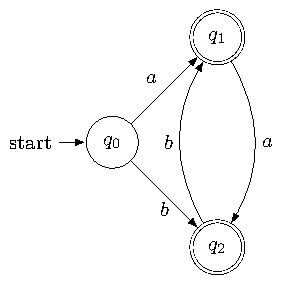
\includegraphics[width=\textwidth]{Min/DFAMinTest-3-1}
        \caption{输入}
        \label{fig:DFAMin-3-1-inside}
    \end{subfigure}
    ~
    \begin{subfigure}[b]{0.4\textwidth}
        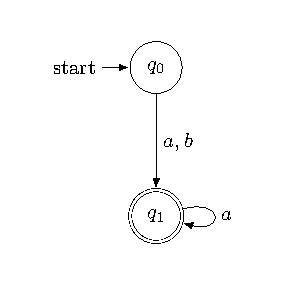
\includegraphics[width=\textwidth]{Min/DFAMinTest-3-3}
        \caption{输出}
        \label{fig:DFAMin-3-3-inside}
    \end{subfigure}
    \caption{DFA::min\_Hopcroft 对第 3 个数据输入输出对比}
    \label{fig:DFAMinHoop-3}
  \end{figure}

对于算法 “DFA::min\_Hopcroft()” 和算法 “DFA::min\_Brzozowski” 的扩展测试见附录。
\chapter{总结}

本文总结如下
\begin{enumerate}
    \item 对于 DFA 中的陷阱状态,可以使用函数 “DFA::usefulf()” 去除;
    \item 除了算法 DFA::min\_Brzozowski() ,其他算法都不能去除 DFA 中的初始不可达状态(start-unreachable);
\end{enumerate}


% DFA::min\_Brzozowski()   
% DFA::min\_Hopcroft()
% DFA::min\_HopcroftUllman()   
% DFA::min\_dragon()
% DFA::min\_Watson()

% 致谢
%!TEX root = ../Demo.tex
\begin{thanksfor}
本文是在段江涛老师的细心指导下完成的。从立题开始,到最终完成,他都给予了我非常多的关怀和帮助,及时纠正我在完成毕业设计期间的犯的错误,提出了非常宝贵的意见。
\end{thanksfor}

%参考文献
%\nocite{*}
\phantomsection%生成该页的链接
\addcontentsline{toc}{chapter}{\bibname}
\bibliographystyle{gbt7714-unsrt}%不对参考文献排序% gbt7714-plain%对参考文献排序 
\bibliography{ThesisFiles/RefFile}%在正文中必须引用,才能显示对应的参考文献

% 附录部分
\appendix
%%!TEX root = ../Demo.tex
\chapter{数据}
这里是附录的数据部分,其实是瞎写;来看个公式编号对不对,如式\eqref{Eq:ApEq1}所示。

\begin{equation}\label{Eq:ApEq1}
h_i = \frac{\max_{j=1}^{N}\{\frac{c_j}{f_j}\}-\frac{c_i}{f_i}}{\max_{j=1}^{N}\{\frac{c_j}{f_j}\}-\min_{j=1}^{N}\{\frac{c_j}{f_j}\}}
\end{equation}

\section{放松一下}
\subsection{惊鸿一面}

\begin{center}
\textbf{惊鸿一面}\cite{shanshui}

{\kaishu 许嵩}

\vspace*{1em}
翻手为云\quad 覆手为雨\\
金盆洗手止风雨\\
不恋红尘\quad 却难舍回忆\\
每一段都有你\\

\vspace*{.7em}
年少初遇\quad 常在我心\\
多年不减你深情\\
江山如画\quad 又怎能比拟\\
你送我的风景\\

\vspace*{.7em}
柳下闻瑶琴\quad 起舞和一曲\\
仿佛映当年\quad 翩若惊鸿影\\
谁三言两语\quad 撩拨了情意\\
谁一颦一笑\quad 摇曳了风景\\

\vspace*{.7em}
纸扇藏伏笔\quad 玄机诗文里\\
紫烟燃心语\quad 留香候人寻\\
史书列豪杰\quad 功过有几许\\
我今生何求\quad 唯你\\

\vspace*{.7em}
远山传来清晨悠然的曲笛\\
晓风掠走光影\\
残月沉霜鬓里\\
有了你\\
恩怨都似飞鸿踏雪泥
\end{center}

\subsection{无题}
\begin{center}
\textbf{无题}

{\kaishu 李商隐}

\vspace*{1em}
相见时难别亦难,东风无力百花残。\\
春蚕到死丝方尽,蜡炬成灰泪始干。\\
晓镜但愁云鬓改,夜吟应觉月光寒。\\
蓬山此去无多路,青鸟殷勤为探看。
\end{center}

\section{代码}
\lstinputlisting[language=C++,caption={C++ code},label=cpp]{./Code/CppTest.cpp}
%标题不编号
\lstinputlisting[language=Java,title={Java code},label=java]{./Code/JavaTest.java}
%无行号
\lstinputlisting[language=Matlab,style=nonumbers]{./Code/floyd.m}


\begin{thebibliography}{A1}
\bibitem[A1]{shanshui}
许嵩. 惊鸿一面[A]. 海蝶音乐. 不如吃茶去[C]. 北京: 北京海蝶音乐有限公司, 2014, 8.

\end{thebibliography}
%%!TEX root = ../Demo.tex
% \chapter*{A 一些基本定义}
% \addcontentsline{toc}{chapter}{A 一些基本定义}
\chapter{一些基本定义}

\begin{convention}[幂集] \label{pro:mathP}
    对于任意集合$A$,我们使用$\mathcal{P}(A)$代表$A$的所有子集。$\mathcal{P}(A)$也叫做$A$的幂集。有时也写作 $2^A$。
\end{convention}

\begin{convention}[函数集]
    对于集合 $A$ 和 $B$ ,$A\longrightarrow B$代表所有从$A$到$B$的函数的集合。而 $ A \not\longrightarrow B$代表所有从$A$到$B$的“partial functions”。
\end{convention}


\begin{remark}
    对于集合$A,B$,关系 $\mathcal{C}\subseteq A \times B$ ,我们可以把$\mathcal{C}$理解为函数 $\mathcal{C} \in A \longrightarrow \mathcal{P}(B)$。
\end{remark}



\begin{convention}[元组投影]
    对于$n$元组 $t=(x_1,x_2,\cdots,x_n)$,我们使用符号${\pi}_i(t)$ $(1 \leq i \leq n)$ 代表元组元素$x_i$;我们使用符号 $\bar{\pi}_i(1 \leq i \leq n)$代表$(n\mbox{-}1)$元组$(x_1,\cdots,x_{i-1},x_{i+1},\cdots,x_n)$。$\pi$ 和 $\bar{\pi}$ 自然扩展到元组集。 
\end{convention}



\begin{convention}[组合关系]
    给出集合$A,B,C$和两个关系$E \subseteq A \times B$ 和 $ F \subseteq B \times C $,定义组合关系(插入操作符$\circ$):
$$ E\circ F = \{ (a,c) : (\exists b:b \in B : (a,b) \in E \land (b,c) \in F) \} $$ 
\end{convention}



\begin{convention}[等价关系的等价类]
    对任何集合 $A$ 上的等价关系 $E$,我们使用 $[A]_E$代表等价类集合,即:
$$ [A]_E = \{ [a]_E :a \in A \} $$
集合 $[A]_E$ 也叫做 $A$ 的由 $E$ 引出的“划分(partition)”。
\end{convention}


\begin{definition}[等价类的指数]
    对于集合$A$上的等价关系$E$,定义$\sharp E = | [A]_E |$。$\sharp E$ 也叫做$E$的“指数”。
\end{definition}


\begin{definition}[字母表] \label{def:Alphabat}
    字母表是有限大小的非空集合。
\end{definition}



\begin{definition}[等价关系的细化]
    对于等价关系$E$和$E'$(在集合$A$上),当且仅当$E \subseteq E'$,$E$是$E'$的“细化”。
\end{definition}

\begin{definition}[划分的细化关系$\sqsubseteq$]
    对于等价关系$E$和$E'$(在集合$A$上),当且仅当$ E \subseteq E' $, $[A]_E$也被称为$ [A]_{E'} $的细化(写作$ [A]_E \sqsubseteq [A]_{E'} $)。当且仅当 $E$ 下的每一个等价类完全包含在$E'$下的某些等价类时,等价命题是$ [A]_E \sqsubseteq [A]_{E'} $ 。
\end{definition}


\begin{definition}[元组和关系反转]
    对一个$n$元组$(x_1,x_2,\cdots,x_n)$,定义反转为函数$R$(后缀和上标)
    $$ (x_1,x_2,\cdots,x_n)^R = (x_n,\cdots,x_2,x_1) $$
给出一个集合元组$A$,定义$A^R = \{ x^R:x\in A \}$。
\end{definition}



%%!TEX root = ../Demo.tex
% \chapter*{B 有限自动机(FA, Finite automata)}
% \addcontentsline{toc}{chapter}{B 有限自动机(FA, Finite automata)}
\chapter{有限自动机}

本节中我们定义有限自动机、其性质及其一些变化。大部分定义直接取自 %\cite{Wats93}。

\begin{definition}[有限自动机($Finite automata,FA$)]
    自动机是一个$6$元组$(Q,V,T,E,S,F)$,其中:
    \begin{itemize}
        \item $Q$ 是有限状态集;
        \item $V$ 是一个字母表;
        \item $ T \in \mathcal{P}(P\times V \times Q) $是一个转换关系;
        \item $ E \in \mathcal{P}(Q\times Q)$ 是一个 $\epsilon$-转换关系(空转换);
        \item $ S \subseteq Q $是开始状态集;
        \item $ F \subseteq Q $是结束状态集;     
    \end{itemize}
    字母表和函数$\mathcal{P}$的定义分别在“定义\ref{def:Alphabat}” 和 “惯例\ref{pro:mathP}”。
\end{definition}


\begin{remark}
    我们也会在状态转换关系的表示上采取一定的自由。例如,我们也把转移关系写成 $T\in V \longrightarrow \mathcal{P}(Q\times Q),T\in Q \times Q \longrightarrow \mathcal{P}(V),T\in Q \times V \longrightarrow \mathcal{P}(Q),T\in Q \longrightarrow \mathcal{P}(V\times Q),E\in Q \longrightarrow \mathcal{P}(Q)$。每种情况下,$Q$的从左到右的顺序会是“preserved”;例如,函数$T\in Q \longrightarrow \mathcal{P}(V \times Q)$ 定义为 $T(p)=\{ (a,q) : (p,a,q) \in T \}$。所使用的签名将从上下文中清除。详见备注 A.3。“$\longrightarrow$ ”的定义出现在惯例 A.2。

    由于本文中我们只考虑有限自动机,所以我们将会频繁的使用简化术语“自动机”。
\end{remark}


% %%%%%%%%%%%%%%%%%%%%%%%%%%%%%%%%%%%%%%%%%%%%%%%%%%%%%%%%%%%%%
% \section*{B.1 $FA$的性质}
% \addcontentsline{toc}{section}{B.1 有限自动机的性质}
\section{有限自动机的性质}
本小节将会定义一些有限自动机(下称$FA$)的性质。为了使定义更加简洁明了,我们引进三个特殊的$FA$: $M=(Q,V,T,E,S,F)$,$M_0=(Q_0,V_0,T_0,E_0,S_0,F_0)$,$ M_1=(Q_1,V_1,T_1,E_1,S_1,F_1) $。

\begin{definition}[$FA$的大小]
    定义一个FA的大小为$|M|=|Q|$。
\end{definition}

\begin{definition}[FA的同构$\cong$]
    我们把同构定义为FA的等价关系。当且仅当 $V_0=V_1$,并且存在双射$g\in Q_0 \longrightarrow Q_1$ ,使得
\begin{itemize}
    \item $T_1 = \{ (g(p,q),a,g(q)) : (p,a,q) \in T_0 \}$
    \item $E_1 = \{ (g(p,q),a,g(q)) : (p,q) \in E_0\}$
    \item $S_1 = \{ g(s):s\in S_0 \}$
    \item $F_1 = \{ g(f):f\in F_0 \}$
\end{itemize}
时$M_0$和$M_1$是同构的(写作$M_0 \cong M_1$)。
\end{definition}
% \newline

\begin{definition}[转移关系$T$的扩展]
    我们把$T \in V \longrightarrow \mathcal{P} (Q \times Q) $ 到 $ T^* \in V^* \longrightarrow \mathcal{P} (Q \times Q)  $的转换关系以如下方式扩展: \\
    \mbox{  } $T^*(\epsilon) = E^*$ \\
    \mbox{且对于 } $(a\in V,w\in V^*)$ \mbox{ 有 }\\
    \mbox{  } $ T^*(aw) = E^* \circ T(a) \circ T^*(w) $ \\
    操作符$\circ$在惯例 A.5 中定义。\uline{这个定义也可以对称的表示}。
\end{definition}


\begin{remark}
    有时候我们也使用把转移关系写成: $T^* \in Q \times Q \longrightarrow \mathcal{P}(V^*)$。
\end{remark}


\begin{definition}[左语言和右语言]
    状态($M$中)的左语言由函数$ \overleftarrow{\mathcal{L}} _M \in Q \longrightarrow \mathcal{P}(V^*)$ 给出,其中:\\
    \mbox{  } $ \overleftarrow{\mathcal{L}}_M (q) = ( \cup s:s \in S : T^*(s,q) ) $ \\
    状态($M$中)的右语言由函数$ \overrightarrow{\mathcal{L}} _M \in Q \longrightarrow \mathcal{P}(V^*)$给出,其中 \\
    \mbox{  } $ \overrightarrow{\mathcal{L}}_M (q) = ( \cup f:f \in F : T^*(q,f) ) $ \\
    通常在没有歧义的时候移除下标$M$。
\end{definition}


\begin{definition}[$FA$的语言]
    有限自动机的语言由函数 $\mathcal{L}_{FA} \in FA \longrightarrow \mathcal{P}(V^*) $给出,该函数的定义为: \\
    \mbox{   }$ \mathcal{L}_{FA} (M) = (\cup s,f:s \in S \land f \in F : T^* (s,f)) $ 
\end{definition}

\begin{definition}[完全自动机($Complete$)]
    一个完全有限自动机满足 :\\
    \mbox{  } $ Complete(M) \equiv ( \forall q,a:q\in Q \land a \in V : T(q,a) \not= \emptyset )$
\end{definition}

\begin{definition}[$\epsilon$-$free$]
    当且仅当 $E=\emptyset$时,$M$ 是 $\epsilon$-$free$ 的。
\end{definition}

\begin{definition}[Start-useful 自动机]
    一个 $Useful_s$ 有限自动机定义如下: \\
    \mbox{  } $ Useful_s (M) \equiv ( \forall q:q \in Q : \overleftarrow{\mathcal{L}} (q) \not= \emptyset ) $
\end{definition}

\begin{definition}[Final-useful 自动机]
    一个 $Useful_f$ 有限自动机定义如下: \\
    \mbox{  } $ Useful_f (M) \equiv ( \forall q:q \in Q : \overrightarrow{\mathcal{L}} (q) \not= \emptyset ) $
\end{definition}

\begin{remark}
    $Useful_s$和$Useful_f$与 $FA$ 的反转密切相关(见变换 B.22),对所有的 $M \in FA$,有 $Useful_f (M) \equiv Useful_s (M^R)$。
\end{remark}

\begin{definition}[Useful 自动机]
    $Useful$ 有限自动机是一个只有可达状态的有限自动机:\\
    \mbox{  } $ Useful (M) \equiv Useful_s (M) \land Useful_f (M) $ 
\end{definition}

\begin{property}[确定性有限自动机($DFA$)]
    当且仅当
    \begin{itemize}
    \item  无多重初始状态;
    \item  无$\epsilon$转移;
    \item  转移函数$T \in Q \times V \longrightarrow \mathcal{P} (Q) $ 不将 $Q \times V$ 映射至多重状态。
\end{itemize}
时有限自动机$M$是确定性的。形式表达为:
$$ Det(M) \equiv ( |S| \leq 1 \land \epsilon-free(E) \land ( \forall q,a:q \in Q \land a \in V : |T(q,a)| \leq 1 )) $$
\end{property}

\begin{definition}[$FA$的确定性]
    $DFA$代表所有确定性的有限自动机的集合。我们把$FA \setminus DFA$称为非确定性有限自动机($NDFA$,$nondeterministic\ finite\ automata$)的集合。
\end{definition}

\begin{convention}[DFA的转换函数]
    对于$(Q,V,T,\emptyset,S,F)\in DFA$,我们考虑把转换函数记为$T\in Q \times V \not\rightarrow Q$($\not\rightarrow$的定义可以查看惯例A.2)。当且仅当 $DFA$ 是完全自动机的时候,转换函数是全函数。
\end{convention}


\begin{property}[弱确定性自动机]
    一些作者用比$Det$弱的确定性自动机的定义;使用左语言,定义如下:
    $$ Det'(M) \equiv (\forall q_0,q_1 : q_0 \in Q \land q_1 \in Q \land q_0 \not= q_1 : \overleftarrow{\mathcal{L}}(q_0) \cap \overleftarrow{\mathcal{L}}(q_1) = \emptyset ) $$
很容易证明$Det(M) \Rightarrow Det'(M)$。
\end{property}

\begin{definition}[$DFA$的最小化]
    满足以下条件时,$M\in DFA$是最小化的:
    $$ Min(M) \equiv (\forall M' : M' \in DFA \land Complete(M') \land \mathcal{L}(M) = \mathcal{L}_{FA}(M') : |M| \leq |M'| ) $$
$Min$仅定义在$DFA$上。如果我们定义一个最小的但是仍然完全的$DFA$,那么一些定义将会更加简单。它的定义如下:
\small{ $$ Min_{\mathcal{C}}(M) \equiv ( \forall M':M' \in DFA \land Complete(M') \land \mathcal{L}_{FA}(M) = \mathcal{L}_{FA}(M'): |M| \leq |M'| ) $$ }
$Min_{\mathcal{C}}$仅定义在完全$DFA$上。
\end{definition}

\begin{definition}[$DFA$的最小化]
    根据 Myhill-Nerode 定理,\CJKunderline{An M, such that Min(M)},是唯一的最小化$DFA$,定理的相关介绍在 \cite{watson1993taxonomyb}。
\end{definition}

\begin{property}[$DFA$最小化的一个替代定义]
    为了最小化$DFA$,使用定义(仅定义在$DFA$上):
    \begin{align*}
        Minimal(Q,V,T,\emptyset,S,F)  \equiv & ( \forall q_0,q_1:q_0 \in Q \land q_1 \in Q \land q_0 \not= q_1 : \overrightarrow{\mathcal{L}}(q_0) \not= \overrightarrow{\mathcal{L}}(q_1)  ) \\
                                     & \land Useful(Q,V,T,\emptyset,S,F)
        \end{align*}
% \mbox{  }$Minimal(Q,V,T,\emptyset,S,F) \equiv  ( \forall q_0,q_1:q_0 \in Q \land q_1 \in Q \land q_0 \not= q_1 : \overrightarrow{\mathcal{L}}(q_0) \not= \overrightarrow{\mathcal{L}}(q_1)  )$ \\
% \mbox{              } $\land Useful(Q,V,T,\emptyset,S,F)$ \\
有 $Minimal(M) \equiv Min(M)$(对所有$M\in DFA$)。很容易证明$Min(M)$ $\Rightarrow$ $Minimal(M)$。\uline{The reverse direction follows from the Myhill-Nerode 定理}。

与$Min_{\mathcal{C}}$相似的定义是(同样也只定义在$DFA$上):
    \begin{align*}
        Minimal_{\mathcal{C}}(Q,V,T,\emptyset,S,F)  \equiv & ( \forall q_0,q_1:q_0 \in Q \land q_1 \in Q \land q_0 \not= q_1 : \overrightarrow{\mathcal{L}}(q_0) \not= \overrightarrow{\mathcal{L}}(q_1)  ) \\
                                 & \land Useful(Q,V,T,\emptyset,S,F)
    \end{align*}
% \mbox{  }$Minimal_{\mathcal{C}}(Q,V,T,\emptyset,S,F) \equiv  ( \forall q_0,q_1:q_0 \in Q \land q_1 \in Q \land q_0 \not= q_1 : \overrightarrow{\mathcal{L}}(q_0) \not= \overrightarrow{\mathcal{L}}(q_1)  )$ \\
% \mbox{              } $\land Useful_s (Q,V,T,\emptyset,S,F)$ \\
有 $Minimal_{\mathcal{C}}(M) \equiv Min_{\mathcal{C}}(M)$的性质(对于所有的$M\in DFA$)。很容易证明$Min_{\mathcal{C}}(M)$ $\Rightarrow$ $Minimal_{\mathcal{C}}(M)$。\uline{The reverse direction follows from the Myhill-Nerode 定理}。
\end{property}


% %%%%%%%%%%%%%%%%%%%%%%%%%%%%%%%%%%%%%%%%%%%%%%%%%%%%%%%%%%%%%%%%%%%%
% \section*{B.2 有限自动机的变换}
% \addcontentsline{toc}{section}{B.2 有限自动机的变换}
% \clearpage
\section{有限自动机的变换}

\begin{transformation}[$FA$ 反转]
    $FA$反转由上标函数$ R \in FA \longrightarrow FA $ 给出,它的定义如下:
    $$ (Q,V,T,S,F)^R = (Q,V,T^R,E^R,F,S) $$ 
函数 $R$ 满足
$$(\forall M : M \in FA : ( \mathcal{L} (M) )^R = \mathcal{L}_{FA}(M^R)) $$
\end{transformation}

\begin{transformation}[移除开始状态不可达状态]
    变换$useful_s \in FA \longrightarrow FA$移除开始状态不可达状态:
    \begin{table}[!htbp]
        \centering
        \small% fontsize
        \setlength{\tabcolsep}{4pt}% column separation
        \renewcommand{\arraystretch}{1.62}%row space 
        \begin{tabular}{lcll} 
            $useful_s(Q,V,T,E,S,F)$ & = & {\bfseries let} & $U = SReachable(Q,V,T,E,S,F)$ \\
                                    &   & {\bfseries in}  &                               \\
                                    &   &                 & $(U,V,T \cap (U\times V \times U), E \cap (U \times U), S \cap U, F \cap U )$  \\
                                    &   & {\bfseries end} &                               \\
        \end{tabular}
    \end{table}
\\函数 $ useful_s $满足
$$ (\forall M : M \in FA : Useful_s ( useful_s(M) ) \land \mathcal{L}_{FA} (useful_s(M)) = \mathcal{L}_{FA}(M)) $$
\end{transformation}

\begin{transformation}[子集构造]
    函数$subset$把一个$\epsilon$-$free$ $FA$ 转换为一个 $DFA$ (in the \textbf{let} clause $T'\in \mathcal{P}(Q) \times V \longrightarrow \mathcal{P}(\mathcal{P} (Q) )$): 
    \begin{table}[!htbp]
        \centering
        %\small% fontsize
        \setlength{\tabcolsep}{4pt}% column separation
        \renewcommand{\arraystretch}{1.62}%row space 
        \begin{tabular}{lcll} 
            $subset(Q,V,T,\emptyset,S,F)$ & = & {\bfseries let} & $T'(U,a) = \{ (q:q\in U : T(q,a) ) \} $ \\
                                          &   &                 & $F'= \{ U : U \in \mathcal{P}(Q) \land U \cap F \not= \emptyset \} $ \\
                                          &   & {\bfseries in}  &                                         \\
                                          &   &                 & $ ( \mathcal{P}(Q),V,T',\emptyset,\{ S \},F' ) $  \\
                                          &   & {\bfseries end} &                               \\
        \end{tabular}
    \end{table}
    \\有时候也把它说成“幂集”构造。
\end{transformation}

\begin{property}[子集构造]
    设 $M_0=( Q_0,v,t_0,\emptyset,S_0,F_0 )$和 $M_1 = subset(M_0)$为有限自动机。通过子集构造,状态集$M_1$成为$\mathcal{P}(Q_0)$。有如下性质:
    $$ (\forall p:p \in \mathcal{P}(Q_0) : \overrightarrow{\mathcal{L}}_{M_1}(p) = ( q:q \in p : \overrightarrow{\mathcal{L}}_{M_1}(q) ) ) $$
\end{property}



\begin{definition}[优化子集构造]
    函数$subsetopt$把一个$\epsilon$-$free$ $FA$ 转换为一个 $DFA$ 。此函数是$subset$的一个优化版本:
    \begin{table}[!htbp]
        \centering
        %\small% fontsize
        \setlength{\tabcolsep}{4pt}% column separation
        \renewcommand{\arraystretch}{1.62}%row space 
        \begin{tabular}{lcll} 
            $subset(Q,V,T,\emptyset,S,F)$ & = & {\bfseries let} & $ T'(U,a) = \{ (q:q\in U : T(q,a) ) \} $ \\
                                          &   &                 & $ Q' = \mathcal{P} (Q) \setminus \{ \emptyset \} $ \\
                                          &   &                 & $ F'= \{ U : U \in \mathcal{P}(Q) \land U \cap F \not= \emptyset \} $ \\
                                          &   & {\bfseries in}  &                                         \\
                                          &   &                 & $ ( Q',V,T' \cap (Q' \times V \times Q'),\emptyset,\{ S \},F' ) $  \\
                                          &   & {\bfseries end} &                               \\
        \end{tabular}
    \end{table}
    \\除了性质$\mathcal{L}_{FA} (subsetopt(M)) = \mathcal{{L}} (M) $(对所有的$M\in FA$)之外,函数$subsetopt$还满足
    $$ ( \forall M : M \in FA \land \epsilon \mbox{-}free(M) : Det(subset(M)) )  $$
\end{definition}





%!TEX root = ../Demo.tex
\chapter{自动机状态转移图}

%%  接受{$\mathcal{L}$}=0*10*的自动机{\cite[fig 5-4]{book1}}

\begin{figure}[!htbp]
    \centering
    \begin{subfigure}[b]{0.35\textwidth}
        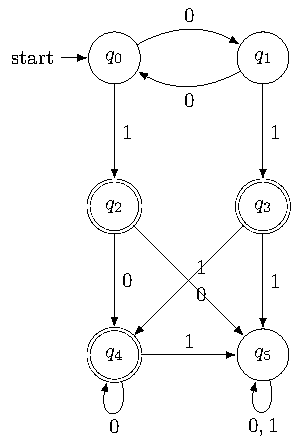
\includegraphics[width=\textwidth]{automaton_4_0}
        \caption{}
        \label{fig:DFA4_0}
    \end{subfigure}
    ~
    \begin{subfigure}[b]{0.35\textwidth}
        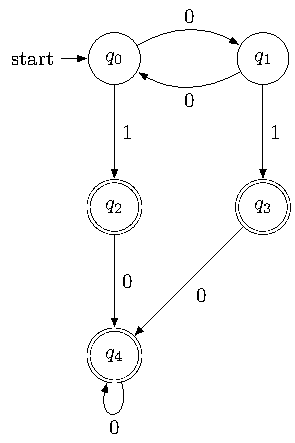
\includegraphics[width=\textwidth]{automaton_4_1}
        \caption{}
        \label{fig:DFA4_1}
    \end{subfigure}
    \\
    \begin{subfigure}[b]{0.35\textwidth}
        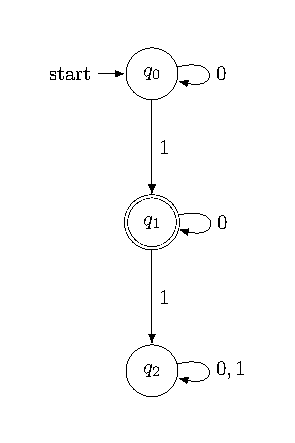
\includegraphics[width=\textwidth]{automaton_4_2}
        \caption{}
        \label{fig:DFA4_2}
    \end{subfigure}
    ~
    \begin{subfigure}[b]{0.35\textwidth}
        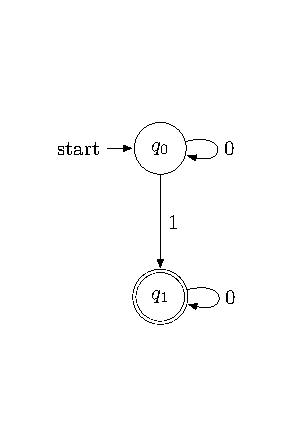
\includegraphics[width=\textwidth]{automaton_4_3}
        \caption{}
        \label{fig:DFA4_3}
    \end{subfigure}
    \caption{(a)接受{$\mathcal{L}$}=0*10*的自动机{\cite[fig 5-4]{book1}};  (b) 图(a)去除非 “final-reachable” 状态 {$q_5$}; (c) 与图(a) 的 $DFA$ 同构的含有陷阱状态的最小 $DFA$ ;(d) 与图(a) 的 $DFA$ 同构的不含陷阱状态的最小 $DFA$。}
    \label{fig:DFA4}
\end{figure}


\begin{figure}[!htbp]
    \centering
    \begin{subfigure}[b]{0.3\textwidth}
        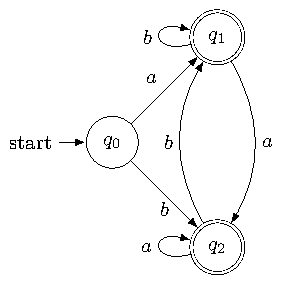
\includegraphics[width=\textwidth]{Min/DFAMinTest-3-0}
        \caption{}
        \label{fig:DFAMin-3-0}
    \end{subfigure}
    ~
    \begin{subfigure}[b]{0.3\textwidth}
        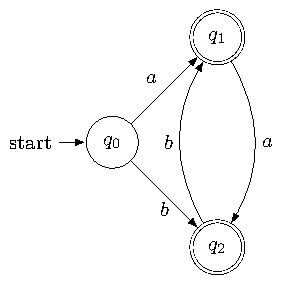
\includegraphics[width=\textwidth]{Min/DFAMinTest-3-1}
        \caption{}
        \label{fig:DFAMin-3-1}
    \end{subfigure}
    ~
    \begin{subfigure}[b]{0.3\textwidth}
        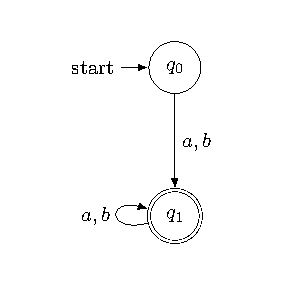
\includegraphics[width=\textwidth]{Min/DFAMinTest-3-2}
        \caption{}
        \label{fig:DFAMin-3-2}
    \end{subfigure}
    \caption{(a)一个 DFA; (b) 图(a)去除转移关系$T=\{(1 \times \mbox{'b'} \times 1),(2 \times \mbox{'a'} \times 2)\}$ 后的最小的 DFA ; (c) 与图(a) 同构的最小的 DFA }
    \label{fig:DFAMin-3}
  \end{figure}

  \begin{figure}[!htbp]
    \centering
    \begin{subfigure}[b]{0.9\textwidth}
        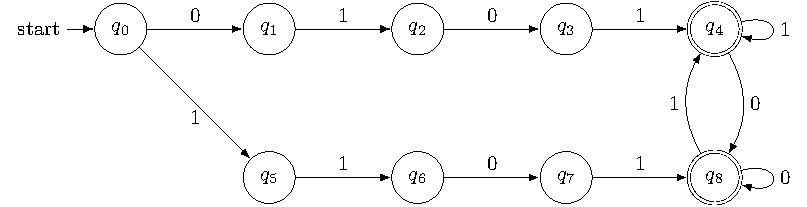
\includegraphics[width=\textwidth]{Min/DFAMinTest-5-0}
        \caption{}
        \label{fig:DFAMin-5-0}
    \end{subfigure}
    \\
    \begin{subfigure}[b]{0.9\textwidth}
        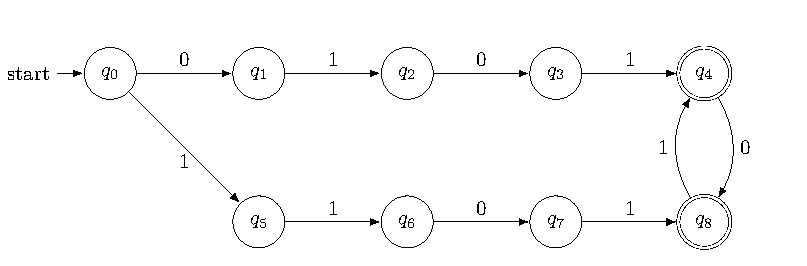
\includegraphics[width=\textwidth]{Min/DFAMinTest-5-1}
        \caption{}
        \label{fig:DFAMin-5-1}
    \end{subfigure}
    \\
    \begin{subfigure}[b]{0.9\textwidth}
        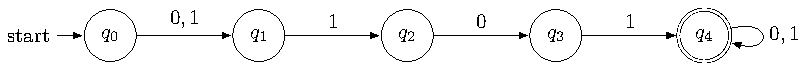
\includegraphics[width=\textwidth]{Min/DFAMinTest-5-2}
        \caption{}
        \label{fig:DFAMin-5-2}
    \end{subfigure}
    \caption{(a)一个 DFA; (b) 图(a)去除转移关系$T=\{(4 \times \mbox{'1'} \times 4),( 8 \times \mbox{'0'} \times 8 )\}$ 后的最小的 DFA ; (c) 与图(a) 同构的最小的 DFA }
    \label{fig:DFAMin-5}
  \end{figure}


  \begin{figure}[!htbp]
    \centering
    \begin{subfigure}[b]{0.7\textwidth}
        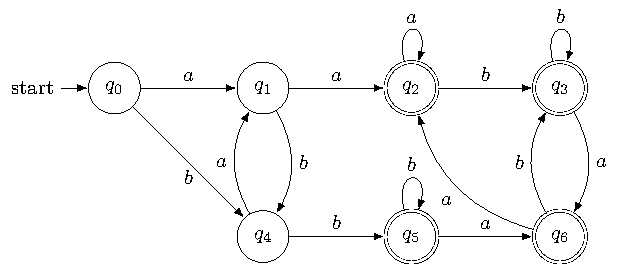
\includegraphics[width=\textwidth]{Min/DFAMinTest-4-0}
        \caption{}
        \label{fig:DFAMin-4-0}
    \end{subfigure}
    \\
    \begin{subfigure}[b]{0.7\textwidth}
        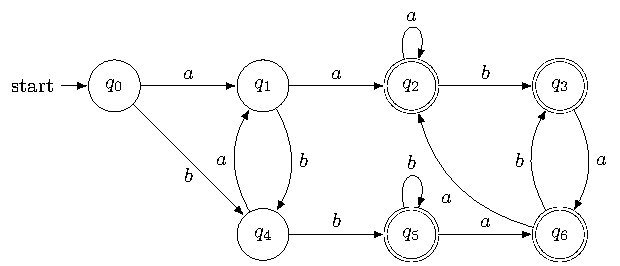
\includegraphics[width=\textwidth]{Min/DFAMinTest-4-1}
        \caption{}
        \label{fig:DFAMin-4-1}
    \end{subfigure}
    \\
    \begin{subfigure}[b]{0.7\textwidth}
        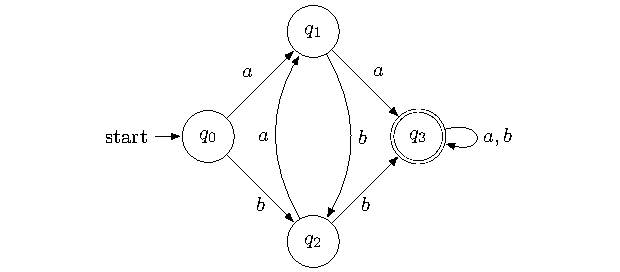
\includegraphics[width=\textwidth]{Min/DFAMinTest-4-2}
        \caption{}
        \label{fig:DFAMin-4-2}
    \end{subfigure}
    \caption{(a)一个 DFA; (b) 图(a)去除转移关系$T=\{(3 \times \mbox{'b'} \times 3)\}$ 后的最小的 DFA ; (c) 与图(a) 同构的最小的 DFA }
    \label{fig:DFAMin-4}
  \end{figure}

\begin{figure}[!htbp]
  \centering
  \begin{subfigure}[b]{0.35\textwidth}
      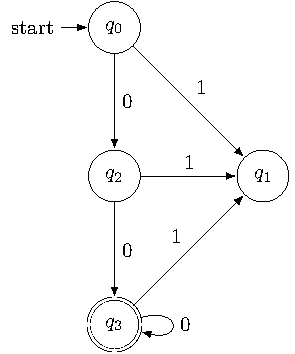
\includegraphics[width=\textwidth]{usefulf2-1}
      \caption{}
      \label{fig:usefulf2-1}
  \end{subfigure}
  ~
  \begin{subfigure}[b]{0.35\textwidth}
      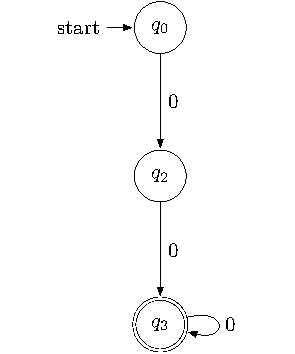
\includegraphics[width=\textwidth]{usefulf2-2}
      \caption{}
      \label{fig:usefulf2-2}
  \end{subfigure}
  \caption{(a)接受{$\mathcal{L}$}=000*的最小的 DFA;  (b) 图(a)去除非 “final-reachable” 状态 {$q_1$}; }
  \label{fig:usefulf2-0}
\end{figure}




\begin{figure}[!htbp]
    \centering
    \begin{subfigure}[b]{0.7\textwidth}
        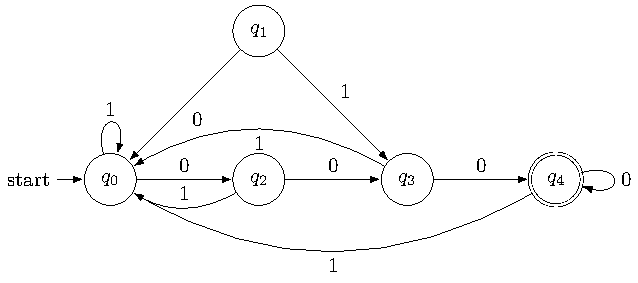
\includegraphics[width=\textwidth]{keepMin/mindfa1-with-start-unreachable}
        \caption{}
        \label{fig:keepMin-1-unreachable}
    \end{subfigure}
    \\
    \begin{subfigure}[b]{0.7\textwidth}
        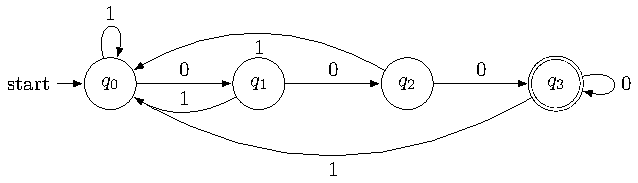
\includegraphics[width=\textwidth]{keepMin/mindfa1}
        \caption{}
        \label{fig:keepMin-1-nonTheState}
    \end{subfigure}
    \caption{(a)接受{$\mathcal{L}=\{ x000 | x \in \{ 0,1\}^{*} \}$}的最小的 DFA;  (b) 图(a)去除开始不可达状态 {$q_1$}; }
    \label{fig:keepMin-1}
\end{figure}

\begin{figure}[!htbp]
    \centering
    \begin{subfigure}[b]{0.7\textwidth}
        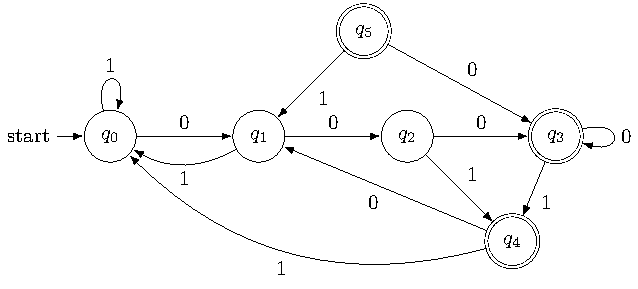
\includegraphics[width=\textwidth]{keepMin/mindfa2-with-start-unreachable}
        \caption{}
        \label{fig:keepMin-2-unreachable}
    \end{subfigure}
    \\
    \begin{subfigure}[b]{0.7\textwidth}
        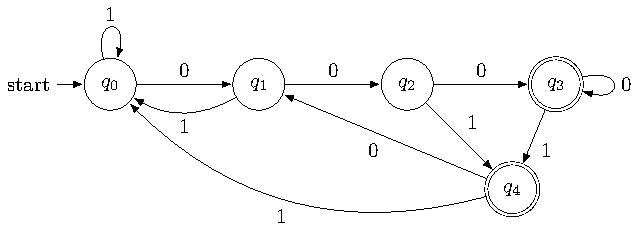
\includegraphics[width=\textwidth]{keepMin/mindfa2}
        \caption{}
        \label{fig:keepMin-2-nonTheState}
    \end{subfigure}
    \caption{(a)接受{$\mathcal{L}=\{ x000 | x \in \{ 0,1\}^{*} \cup \{ x001 | x \in \{ 0,1\}^{*} \}$}的最小的 DFA;  (b) 图(a)去除开始不可达状态 {$q_5$}; }
    \label{fig:keepMin-2}
\end{figure}

\begin{figure}[!htbp]
    \centering
    \begin{subfigure}[b]{0.9\textwidth}
        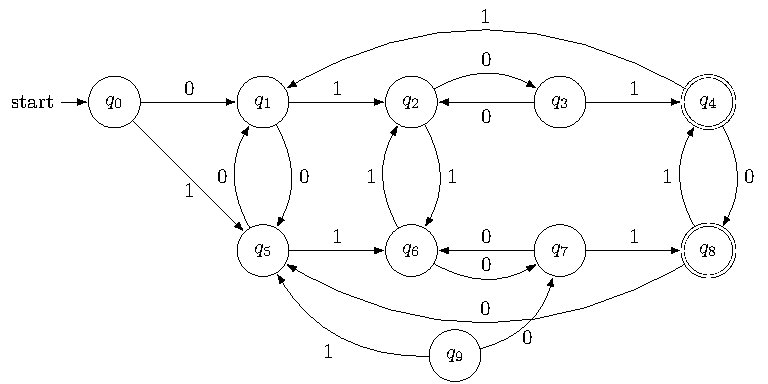
\includegraphics[width=\textwidth]{DFA11-0}
        \caption{}
        \label{fig:DFA11-0}
    \end{subfigure}
    \\
    \begin{subfigure}[b]{0.9\textwidth}
        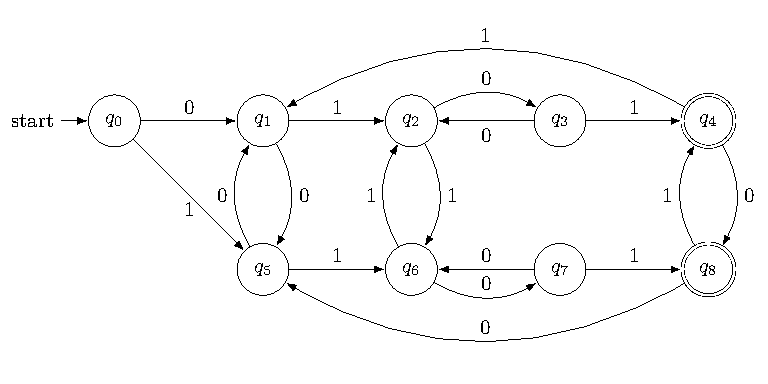
\includegraphics[width=\textwidth]{DFA11-1}
        \caption{}
        \label{fig:DFA11-1}
    \end{subfigure}
    \\
    \begin{subfigure}[b]{0.9\textwidth}
        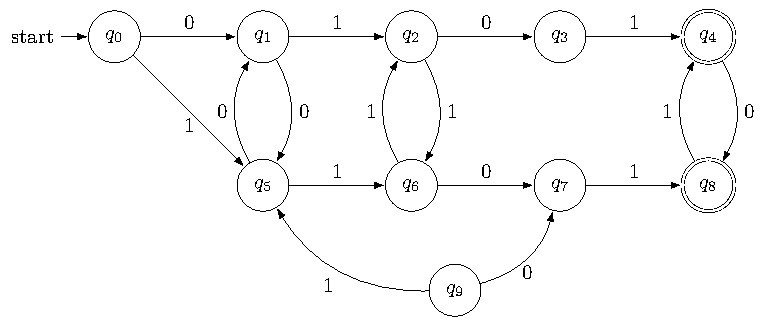
\includegraphics[width=\textwidth]{DFA11-2}
        \caption{}
        \label{fig:DFA11-2}
    \end{subfigure}
    \caption{(a)一个最小的DFA;  (b) 图(a) 移除开始不可达状态 {$q_9$};(c) 图(a)移除转移关系$T=\{(4 \times '1' \times 1),(8 \times '0' \times 5),(3 \times '0' \times 2),(7 \times '0' \times 6)\}$后的DFA。 }
    \label{fig:DFA11}
  \end{figure}
%!TEX root = ../Demo.tex
\chapter{算法迭代过程}
\begin{table}[!htbp]
    \caption{图 \ref{fig:DFA11-0} 的 DFA 在 DFA::min\_Hopcroft 算法中的迭代过程}
    \label{tab:hopcroft}
    \centering
    \footnotesize% fontsize
    \setlength{\tabcolsep}{4pt}% column separation
    \renewcommand{\arraystretch}{1.2}%row space 
    \begin{tabular}{ccccccc|cccccccccc|cl} 
        \toprule%\hline 
        \multirow{2}{*}{$n$} & \multirow{2}{*}{状态} & \multirow{2}{*}{$p$} & \multirow{2}{*}{$q$} & \multirow{2}{*}{$L[q]$} & \multirow{2}{*}{$C$} & \multirow{2}{*}{$r$} & \multicolumn{10}{c|}{$L$} & \multirow{2}{*}{$repr$} & \multirow{2}{*}{$\mbox{    }P$}  \\
        \cline{8-17}             &                   &                     &                    &                       &                   &    & 0 & 1 &2 &3 &4 &5 &6 &7 & 8 & 9 & & \\
        %                        &        & \multicolumn{4}{c}{输入字符} \\
        %\cline{3-6}  {状态说明}  & {状态} &$a$ & $b$ & $1$ & $\epsilon$ \\
        \midrule%\hline
        \multirow{2}{*}{1} & 前 & 0 & 4 & 1 & 1 & -  & 0 & 0 & 0 & 0 & 1 & 0 & 0 & 0 & 0 & 0 & \{0,4\} & \{0,1,2,3,5,6,7,9\},\{4,8\} \\
                           & 后 & 0 & 4 & 1 & 1 & 3  & 0 & 0 & 0 & 2 & 1 & 0 & 0 & 0 & 0 & 0 & \{0,4\} & \{0,1,2,5,6,9\},\{3,7\},\{4,8\} \\
        \midrule
        \multirow{2}{*}{2} & 前 & 4 & 4 & 1 & 1 & -  & 0 & 0 & 0 & 2 & 1 & 0 & 0 & 0 & 0 & 0 & \{0,4\} & \{0,1,2,5,6,9\},\{3,7\},\{4,8\} \\
                           & 后 & 4 & 4 & 2 & 1 & 8  & 0 & 0 & 0 & 2 & 2 & 0 & 0 & 0 & 1 & 0 & \{0,4\} & \{0,1,2,5,6,9\},\{3,7\},\{4\},\{8\} \\
        \midrule
        \multirow{2}{*}{3} & 前 & 0 & 3 & 1 & 1 & -  & 0 & 0 & 0 & 1 & 2 & 0 & 0 & 0 & 1 & 0 & \{0,3,4,8\} & \{0,1,2,5,6,9\},\{3,7\},\{4\},\{8\} \\
                           & 后 & 0 & 3 & 1 & 1 & -1 & 0 & 0 & 0 & 1 & 2 & 0 & 0 & 0 & 1 & 0 & \{0,3,4,8\} & \{0,1,2,5,6,9\},\{3,7\},\{4\},\{8\} \\
        \midrule
        
        \multirow{2}{*}{4} & 前 & 3 & 3 & 1 & 1 & -  & 0 & 0 & 0 & 1 & 2 & 0 & 0 & 0 & 1 & 0 & \{0,3,4,8\} & \{0,1,2,5,6,9\},\{3,7\},\{4\},\{8\} \\
                           & 后 & 3 & 3 & 1 & 1 & -1 & 0 & 0 & 0 & 1 & 2 & 0 & 0 & 0 & 1 & 0 & \{0,3,4,8\} & \{0,1,2,5,6,9\},\{3,7\},\{4\},\{8\} \\
        \midrule
        \multirow{2}{*}{5} & 前 & 4 & 3 & 1 & 1 & -  & 0 & 0 & 0 & 1 & 2 & 0 & 0 & 0 & 1 & 0 & \{0,3,4,8\} & \{0,1,2,5,6,9\},\{3,7\},\{4\},\{8\} \\
                           & 后 & 4 & 3 & 1 & 1 & -1 & 0 & 0 & 0 & 1 & 2 & 0 & 0 & 0 & 1 & 0 & \{0,3,4,8\} & \{0,1,2,5,6,9\},\{3,7\},\{4\},\{8\} \\
        \midrule
        \multirow{2}{*}{6} & 前 & 8 & 3 & 1 & 1 & -  & 0 & 0 & 0 & 1 & 2 & 0 & 0 & 0 & 1 & 0 & \{0,3,4,8\} & \{0,1,2,5,6,9\},\{3,7\},\{4\},\{8\} \\
                           & 后 & 8 & 3 & 1 & 1 & -1 & 0 & 0 & 0 & 1 & 2 & 0 & 0 & 0 & 1 & 0 & \{0,3,4,8\} & \{0,1,2,5,6,9\},\{3,7\},\{4\},\{8\} \\
        \midrule
        \multirow{2}{*}{7} & 前 & 0 & 3 & 0 & 0 & -  & 0 & 0 & 0 & 0 & 2 & 0 & 0 & 0 & 1 & 0 & \{0,3,4,8\} & \{0,1,2,5,6,9\},\{3,7\},\{4\},\{8\} \\
                           & 后 & 0 & 3 & 0 & 0 & 2  & 2 & 0 & 0 & 0 & 2 & 0 & 0 & 0 & 1 & 0 & \{0,3,4,8\} & \{0,1,5\},\{2,6,9\}\{3,7\},\{4\},\{8\} \\
        \midrule
        \multirow{2}{*}{8} & 前 & 3 & 3 & 0 & 0 & -  & 2 & 0 & 0 & 0 & 2 & 0 & 0 & 0 & 1 & 0 & \{0,3,4,8\} & \{0,1,5\},\{2,6,9\},\{3,7\},\{4\},\{8\} \\
                           & 后 & 3 & 3 & 0 & 0 & -1 & 2 & 0 & 0 & 0 & 2 & 0 & 0 & 0 & 1 & 0 & \{0,3,4,8\} & \{0,1,5\},\{2,6,9\},\{3,7\},\{4\},\{8\} \\
        \midrule
        \multirow{2}{*}{9} & 前 & 4 & 3 & 0 & 0 & -  & 2 & 0 & 0 & 0 & 2 & 0 & 0 & 0 & 1 & 0 & \{0,3,4,8\} & \{0,1,5\},\{2,6,9\},\{3,7\},\{4\},\{8\} \\
                           & 后 & 4 & 3 & 0 & 0 & -1 & 2 & 0 & 0 & 0 & 2 & 0 & 0 & 0 & 1 & 0 & \{0,3,4,8\} & \{0,1,5\},\{2,6,9\},\{3,7\},\{4\},\{8\} \\
        \midrule
        \multirow{2}{*}{10}& 前 & 8 & 3 & 0 & 0 & -  & 2 & 0 & 0 & 0 & 2 & 0 & 0 & 0 & 1 & 0 & \{0,3,4,8\} & \{0,1,5\},\{2,6,9\},\{3,7\},\{4\},\{8\} \\
                           & 后 & 8 & 3 & 0 & 0 & -1 & 2 & 0 & 0 & 0 & 2 & 0 & 0 & 0 & 1 & 0 & \{0,3,4,8\} & \{0,1,5\},\{2,6,9\},\{3,7\},\{4\},\{8\} \\
        \midrule
        \multirow{2}{*}{11}& 前 & 0 & 0 & 1 & 1 & -  & 1 & 0 & 0 & 0 & 2 & 0 & 0 & 0 & 1 & 0 & \{0,2,3,4,8\} & \{0,1,5\},\{2,6,9\},\{3,7\},\{4\},\{8\} \\
                           & 后 & 0 & 0 & 2 & 1 & 1  & 2 & 0 & 0 & 0 & 2 & 0 & 0 & 0 & 1 & 0 & \{0,2,3,4,8\} & \{0\},\{1,5\},\{2,6,9\},\{3,7\},\{4\},\{8\} \\
        \midrule
        
        \multirow{2}{*}{12}& 前 & 2 & 0 & 2 & - & -  & - & - & - & - & - & - & - & - & - & - & -             & ------ \\
                           & 后 & - & - & - & - & -  & - & - & - & - & - & - & - & - & - & - & -             & ------ \\
        %\midrule
        \bottomrule%\hline 
    \end{tabular}
\end{table}

表 \ref{tab:hopcroft} 中的表头与 FIRE engine 中 Hopcroft 算法的实现中的变量一一对应。其中
\begin{itemize}
    \item $n$ 为迭代次数(FIRE engine 中无此变量,为了方便描述算法迭代过程添加);
    \item “状态”意指进行等价类分割前和等价类分割后;
    \item $p$ 为当前要进行等价类分割的等价类;
    \item $q$ 为等价类分割的参数,$q \in Q$;
    \item L[q] 作为函数 C.iterator(L[q]) 的参数;
    \item $C$ 为等价类分割的参数,$C \in V$;
    \item $r$ 为分割开的等价类的代表;
    \item $L$ 为 Hopcroft 算法中的 $L$;
    \item $repr$ 为 等价类代表集合,其值为 $P$ 中每个等价类中最小的状态的集合;
    \item $P$ 为等价类集合;
\end{itemize}

\begin{remark}\label{rem:means-of-L}
    Hopcroft 算法(算法 \ref{al:4-8})中的 “$L$” 存储的是二元关系 $F \times V$ 或 $(Q \setminus F) \times V$ , FIRE engine 中的 “$L$” 是一个一维整型数组,其中第 $i$ 个元素的值表示第 $i$ 个状态还需要处理的字符数目。当 FIRE engine 中的 “$L$” 数组内所有元素的值全部为 0 时,算法迭代结束。
\end{remark}
%!TEX root = ../Demo.tex
\chapter{代码}

一个实例化 DFA 类的例子如代码 \ref{lst:DFASample} 所示。代码 \ref{lst:DFASample} 中执行了 DFA::usefulf() 函数,去除多余的状态,让输出数据与原始数据相对应。代码 \ref{lst:DFASample} 对应的 DFA 为图 \ref{fig:keepMin-1-nonTheState} 。


\lstset{style=mystyle}
\begin{lstlisting}[language=C++,label={lst:DFASample},caption={实例化DFA示例}]
#include"DFA.h"
#include<iostream>
int main()
{
    DFA_components dfa_com1;

    // StateSet S  开始状态集
    dfa_com1.S.set_domain(4);
    dfa_com1.S.add(0);

    // StateSet F  结束状态集
    dfa_com1.F.set_domain(4);
    dfa_com1.F.add(3);

    // StatePool Q 
    int i = 10;
    while (i--)
    {
        dfa_com1.Q.allocate();
    }

    // DTransRel T transition             
    dfa_com1.T.set_domain(4);
    dfa_com1.T.add_transition(0, '0', 1);
    dfa_com1.T.add_transition(1, '0', 2);
    dfa_com1.T.add_transition(2, '0', 3);
    dfa_com1.T.add_transition(3, '0', 3);
    dfa_com1.T.add_transition(0, '1', 0);
    dfa_com1.T.add_transition(1, '1', 0);
    dfa_com1.T.add_transition(2, '1', 0);
    dfa_com1.T.add_transition(3, '1', 0);

    DFA dfa1(dfa_com1);

    std::cout<<dfa1<<std::endl;
	
    return 0;
}
\end{lstlisting}
\chapter{DFA::min\_Hopcroft() 的扩展测试}
本文对 DFA::min\_Hopcroft 算法的更改进行测试对比说明。由代码 \ref{list:hop} 更改为代码 \ref{list:hopedit}
\lstset{style=mystyle}
\begin{lstlisting}[language=c++,label={list:hop},caption={原始的 Hopcroft}]
    // mark this element of L as processed. ([q],c)
    L[q]--;

    // Iterate over all eq. classes, and try to split them.
    State p;
    repr = P.representatives(); // all partitions(eq.classes)
    for (repr.iter_start(p); !repr.iter_end(p); repr.iter_next(p))
    {
        // Now split [p] w.r.t (q, C_(L[q]))
        State r(split(p, q, C.iterator(L[q]), P)); 
\end{lstlisting}

%\lstset{style=mystyle}
\begin{lstlisting}[language=c++,label={list:hopedit},caption={更改后的 Hopcroft}]
    // mark this element of L as processed. ([q],c)
    L[q]--;
    CharRange c = C.iterator(L[q]); // 记录正在处理的c      //新增位置

    // Iterate over all eq. classes, and try to split them.
    State p;
    repr = P.representatives(); // all partitions(eq.classes)
    for (repr.iter_start(p); !repr.iter_end(p); repr.iter_next(p))
    {
        // Now split [p] w.r.t (q, C_(L[q]))
        State r(split(p, q, c, P));                       //更改位置
\end{lstlisting}


\begin{figure}[!htbp]
    \centering
    \begin{subfigure}[b]{0.49\textwidth}
        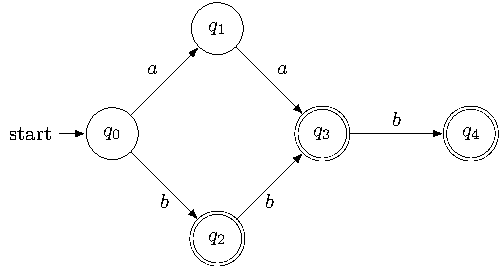
\includegraphics[width=\textwidth]{keepMin/hoperror--1}
        \caption{$\mathcal{L}=\{aa \cup aab \cup b \cup bb \cup bbb\}$}
        \label{fig:hoperror--1}
    \end{subfigure}
    ~
    \begin{subfigure}[b]{0.49\textwidth}
        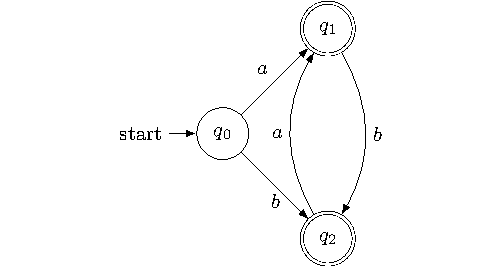
\includegraphics[width=\textwidth]{keepMin/hoperror--2}
        \caption{}
        \label{fig:hoperror--2}
    \end{subfigure}
    \\
    \begin{subfigure}[b]{0.7\textwidth}
        \includegraphics[width=\textwidth]{keepMin/hoperror--3}
        \caption{$\mathcal{L}=\{ab \cup aba\}$}
        \label{fig:hoperror--3}
    \end{subfigure}
    ~
    \begin{subfigure}[b]{0.7\textwidth}
        \includegraphics[width=\textwidth]{keepMin/hoperror--4}
        \caption{$\mathcal{L}=\{ab \cup aba \cup abab\}$}
        \label{fig:hoperror--4}
    \end{subfigure}
    ~
    \begin{subfigure}[b]{0.7\textwidth}
        \includegraphics[width=\textwidth]{keepMin/hoperror--5}
        \caption{$\mathcal{L}=\{aba \cup abab\}$}
        \label{fig:hoperror--5}
    \end{subfigure}
    \caption{一组最小的 DFA }
    \label{fig:hopcerror}
  \end{figure}

以图 \ref{fig:hopcerror} 中的五个最小的 DFA 为数据,测试结果统计如表 \ref{tab:KeepMinResultofAll} 所示

\begin{table}[!htbp]
    \caption{  }
    \label{tab:KeepMinResultofAll}
    \centering
    \small% fontsize
    \setlength{\tabcolsep}{4pt}% column separation
    \renewcommand{\arraystretch}{1.2}%row space 
    \begin{tabular}{l|p{4em}<{\centering} p{4em}<{\centering} p{4em}<{\centering} p{4em}<{\centering} p{4em}<{\centering} }  %l p{3em}<{\centering} p{3em}<{\centering} p{3em}<{\centering}
        \toprule %\hline 
        算法 & \ref{fig:hoperror--1} & \ref{fig:hoperror--2} & \ref{fig:hoperror--3} & \ref{fig:hoperror--4} &  \ref{fig:hoperror--5}  \\
        \midrule
        DFA::min\_Brzozowski()        & $\surd$ & $\surd$ & $\surd$ & $\surd$     & $\surd$        \\
        DFA::min\_Hopcroft()(修改前) & 中止    & $\times$ & $\surd$ & 中止        & $\surd$       \\
        DFA::min\_Hopcroft()(修改后) & $\times$& $\times$& $\surd$ & $\times$    & $\surd$       \\
        DFA::min\_HopcroftUllman()    & $\surd$ & $\surd$ & $\surd$ & $\surd$     & $\surd$       \\
        DFA::min\_dragon()            & $\surd$ & $\surd$ & $\surd$ & $\surd$     & $\surd$       \\
        DFA::min\_Watson()            & $\surd$ & $\surd$ & $\surd$ & $\surd$     & $\surd$       \\
        \bottomrule%\hline  
    \end{tabular}
\end{table}

\newpage
对于图 \ref{fig:hoperror--1} ,修改后 Hopcroft 算法输出如下代码 \ref{FCode1},如图 \ref{fig:hoperror--1-result} 所示。

\begin{lstlisting}[language=bash,label={FCode1},caption={图 \ref{fig:hoperror--1} 输出}]
    DFA
    Q = [0,3)
    S = { 0 }
    F = { 2 }
    Transitions =
    0->{ 'a'->1  'b'->2 }
    1->{ 'a'->2 }
    2->{ 'b'->2 }

    current = -1
\end{lstlisting}
 
对于图 \ref{fig:hoperror--2} ,无论是否修改,Hopcroft均输出代码 \ref{FCode2},如图 \ref{fig:hoperror--2-result} 所示。
\begin{lstlisting}[language=bash,label={FCode2},caption={图 \ref{fig:hoperror--2} 输出}]
    DFA
    Q = [0,2)
    S = { 0 }
    F = { 1 }
    Transitions =
    0->{ ['a','b']->1 }
    1->{ 'b'->1 }

    current = -1
\end{lstlisting}

对于图 \ref{fig:hoperror--4} , 修改后 Hopcroft 输出代码 \ref{FCode4},如图 \ref{fig:hoperror--4-result} 所示。
\begin{lstlisting}[language=bash,label={FCode4},caption={图 \ref{fig:hoperror--4} 输出}]
    DFA
    Q = [0,3)
    S = { 0 }
    F = { 2 }
    Transitions =
    0->{ 'a'->1 }
    1->{ 'b'->2 }
    2->{ 'a'->2 }

    current = -1
\end{lstlisting}


\begin{figure}[!htbp]
    \centering
    \begin{subfigure}[b]{0.7\textwidth}
        \includegraphics[width=\textwidth]{keepMin/hoperror--1-result}
        \caption{$\mathcal{L}=\{aa(b)^* \cup b(b)^*\}$}
        \label{fig:hoperror--1-result}
    \end{subfigure}
    \\
    %\vfill% \vspace{1cm}
    \begin{subfigure}[b]{0.7\textwidth}
        \includegraphics[width=\textwidth]{keepMin/hoperror--2-result}
        \caption{$\mathcal{L}=\{a(b)^* \cup b(b)^*\}$}
        \label{fig:hoperror--2-result}
    \end{subfigure}
    \\
    %\vfill% \vspace{1cm}
    \begin{subfigure}[b]{0.7\textwidth}
        \includegraphics[width=\textwidth]{keepMin/hoperror--4-result}
        \caption{$\mathcal{L}=\{ab(a)^*\}$}
        \label{fig:hoperror--4-result}
    \end{subfigure}
    \caption{Hopcroft 算法的输出 }
    \label{fig:hopcerror-result}
  \end{figure}

  表 \ref{tab:KeepMinResultofAll-hop} 为对比数据

  \begin{table}[!htbp]
    \caption{  }
    \label{tab:KeepMinResultofAll-hop}
    \centering
    \small% fontsize
    \setlength{\tabcolsep}{4pt}% column separation
    \renewcommand{\arraystretch}{1.2}%row space 
    \begin{tabular}{c p{2em}<{\centering}p{2em}<{\centering}ccc }  %l p{3em}<{\centering} p{3em}<{\centering} p{3em}<{\centering}
        \toprule %\hline 
        数据 & $|Q|$ & $|F|$ & $|F|\leq |Q \setminus F|$? & 修改前结果 &  修改后结果  \\
        \midrule
        图 \ref{fig:hoperror--1}        & 5 & 3 & 否 & 中止       & $\times$        \\
        图 \ref{fig:hoperror--2}        & 3 & 2 & 否 & $\times$   & $\times$       \\
        图 \ref{fig:hoperror--3}        & 4 & 2 & 是 & $\surd$    & $\surd$       \\
        图 \ref{fig:hoperror--4}        & 5 & 3 & 否 & 中止       & $\times$       \\
        图 \ref{fig:hoperror--5}        & 5 & 2 & 是 & $\surd$    & $\surd$       \\
        \bottomrule%\hline  
    \end{tabular}
\end{table}

% 图 fig:hopcerror 中的数据在除 Hopcroft 之外的算法的测试中通过,所以本文认为 FIRE engine 对 Hopcroft 算法的实现仍有不足

%l|p{4em}<{\centering} p{4em}<{\centering} p{4em}<{\centering} p{4em}<{\centering} p{4em}<{\centering}

\end{document}

